\documentclass[twocolumn]{aastex63}

\usepackage{enumerate}
\usepackage{amsmath, mathtools}
\usepackage[makeroom]{cancel}
\usepackage{stix}
\usepackage{multirow}
\usepackage{graphicx}
\usepackage{lineno}
\usepackage[normalem]{ulem}
\usepackage{xcolor}
\usepackage{hyperref}
\usepackage{tabularx}
\usepackage{verbatim}
\usepackage{booktabs}
\usepackage{afterpage}
\hypersetup{linkcolor=blue,citecolor=blue,filecolor=cyan,urlcolor=blue}
\usepackage{amsmath}
\usepackage{enumitem}




\newcommand{\gotpm}{\texttt{GOTPM}}
\newcommand{\pgalf}{{\texttt{pGalF}}}
\newcommand{\psb}{{\texttt{PSB}}}
\newcommand{\ramses}{{\texttt{Ramses}}}
\newcommand{\subfind}{{\texttt{SUBFIND}}}
\newcommand{\rockstar}{{\texttt{Rockstar}}}
\newcommand{\cv}{{V_c}}
\newcommand{\mv}{{V_m}}
\newcommand{\lageunha}{\texttt{LagEunha}}
\newcommand{\mpi}{\texttt{MPI}}

%\newcommand{\vel}{\boldsymbol{\mathbf{u}}}
\newcommand{\vel}{{u}}
\newcommand{\surf}[0]{S}
\newcommand{\gradT}[1]{\boldsymbol{\nabla#1}}
\newcommand{\pressure}[0]{\mathcal{P}}

\newcommand{\vect}[1]{\mathbf{#1}}



\shorttitle{\lageunha: a New Cosmological Simulation Code}
\shortauthors{Kim et al.}


\begin{document}

\title{A New Framework for Lagrangian Hydrodynamics with the Laguerre Diagram}
\author[0000-0002-4391-2275]{Juhan Kim}
\affiliation{Center for Advanced Computation, Korea Institute for Advanced Study, Seoul 02455, Republic of Korea}



\correspondingauthor{Juhan Kim}
\email{kjhan@kias.re.kr}

\begin{abstract}
We present \lageunha, a fully Lagrangian hydrodynamics code built
on the Laguerre (power) diagram---a weighted generalization of the
Voronoi tessellation.
Because every cell boundary moves exactly at the local material
velocity, the advection flux $\nabla\!\cdot\!(\phi\vel)$ that
dominates the truncation error in Eulerian and
Arbitrary-Lagrangian--Eulerian (ALE) methods is absorbed
\emph{analytically} into the material derivative, leaving only the
surface pressure--work integral on the right-hand side of the
Euler equations.
Mass, momentum, and energy conservation therefore hold
\emph{by construction} at every time step, without recourse to
advection limiters, remapping diffusion, or Galilean-invariance
corrections.

The scheme used in the tests is the geometric-face scheme (GFS).
Every Laguerre weight is zero, so each face lies on the Voronoi mid-plane.
On an ordinary face the pressure is the MUSCL--HLLC pressure and the face moves at the mean of the two particle velocities.
On an extreme face, where the pressure ratio exceeds $100$ or the lower pressure falls below $10^{-3}$, the pressure and the normal velocity are taken from the Harten--Lax--van Leer average of the conserved state.
GFS is integrated on the Shu--Osher problem, a two-shock collision, a Kelvin--Helmholtz shear layer, a Rayleigh--Taylor layer, and Mach 3 flow past a solid cylinder.
The geometric face velocity keeps the Rayleigh--Taylor energy conserved while the dense spikes reach the lower boundary.
The cylinder wall is a reflecting Riemann problem, and no particle enters the body.
\end{abstract}

\keywords{Galaxy interactions (600), Galaxy encounters (592), Galaxy dark matter halos (1880), Large-scale structure of the universe (902), Cosmic web (330), Galaxy kinematics (602), Dark matter (353), $N$-body simulations (1083)}

%\maketitle



\section{\label{sec:in}Introduction}

Numerical hydrodynamics lies at the heart of modern
astrophysical simulation.
Three broad families of methods are in widespread use:
(i) \emph{Eulerian} codes such as \ramses\ and \textsc{Enzo},
which solve the Euler equations on a fixed or adaptively refined
mesh;
(ii) \emph{Lagrangian} particle methods such as Smoothed Particle
Hydrodynamics \citep[SPH;][]{Lucy1977,GingoldMonaghan1977}
implemented in \textsc{Gadget} and \textsc{Gizmo}; and
(iii) \emph{Arbitrary-Lagrangian--Eulerian} (ALE) or moving-mesh
methods, exemplified by the Voronoi-based code \textsc{Arepo}.
Each approach carries intrinsic trade-offs.
Eulerian schemes require advection fluxes across every cell face
at every time step.  Computing these fluxes demands high-order
reconstruction (WENO, TVD, PPM), yet the truncation error of the
advection operator---proportional to the mesh velocity relative
to the flow---remains the dominant source of numerical diffusion.
ALE methods alleviate this by letting the mesh partially follow
the flow, but a remapping (or mesh-regularization) step is still
needed to prevent cell distortion, and this remapping reintroduces
advective diffusion.
SPH avoids a mesh altogether, but its kernel-based density
estimate introduces smoothing errors that degrade contact
discontinuities and suppress fluid instabilities.

The key observation motivating this work is that
\emph{all} of these difficulties stem from the same root cause:
the need to evaluate or approximate the advection flux
$\nabla\!\cdot\!(\phi\vel)$.
In a \emph{fully Lagrangian} framework, where every cell boundary
moves at the exact material velocity, the advection flux is
absorbed analytically into the Lagrangian (material) derivative.
The conserved form of the Euler equations (eq.~\ref{basic1}) then
reduces to the material-derivative form (eq.~\ref{lag}):
\begin{equation*}
  \mathcal{D}_t^\Omega(\mathsf{U})
  = -\oint_{\partial\Omega}\mathsf{G}_\mathrm{ext}\cdot d\surf
    + \int_\Omega \mathsf{f}_s\,dV,
\end{equation*}
where $\Omega$ is a Lagrangian cell that moves with the flow.
Mass conservation becomes an identity
($\mathcal{D}_t^\Omega(\rho)=0$), momentum and energy are
updated solely through the surface pressure--work integral,
and no advection limiter, remapping operator, or
Galilean-invariance correction is required.
We term this property \emph{self-consistent conservation}:
the conservation laws hold by construction at every stage of the
time integration, as a direct consequence of the Lagrangian
cell definition.

We present \lageunha\ (\textbf{Lag}uerre tessellation
\textbf{E}ngine for the \textbf{Un}iverse with Numerical
\textbf{H}ydrodynamics \textbf{A}lgorithms; ``Eunha'' means
\emph{galaxy} in Korean), a new hydrodynamics code that
realizes this fully Lagrangian ideal.
\lageunha\ tessellates the computational domain with the
\emph{Laguerre} (power) \emph{diagram}---a weighted
generalization of the Voronoi diagram in which each generator
carries an adjustable power distance $\omega_p$.
GFS sets every power distance to zero.
The mesh is then the Voronoi diagram of the particles, and each face moves with the particles.
No remapping step is applied.

The advantages of this fully Lagrangian, self-consistent
framework over the three conventional paradigms are summarized
as follows.

\begin{enumerate}[leftmargin=*,itemsep=2pt]
\item \textbf{Versus Eulerian methods.}---
  The advection flux is eliminated entirely,
  removing the dominant source of numerical diffusion.
  No reconstruction limiter (WENO, TVD) is needed on the
  left-hand side of the equations, and the CFL condition
  involves only the sound speed rather than the sum of
  the flow and sound speeds.
  Spatial resolution adapts automatically with the mass
  distribution, making AMR-style grid refinement unnecessary.

\item \textbf{Versus ALE / moving-mesh methods.}
  No remapping step is applied.
  The cell faces are the Voronoi mid-planes of the particles, and the face velocity used for the $P\,dV$ work is the velocity of that mid-plane except on an extreme face.

\item \textbf{Versus SPH.}---
  Cell-averaged densities are exact by construction
  ($\rho_p = m_p/\Omega_p$), whereas SPH estimates density
  through a kernel sum that introduces smoothing errors.
  Contact discontinuities and fluid instabilities are
  therefore resolved sharply from the outset.
  The face-based pressure evaluation provides a natural
  framework for Riemann solvers and high-order face
  interpolations that are difficult to formulate in the
  kernel-based SPH context.
\end{enumerate}

The hydrodynamics scheme in this paper is the geometric-face scheme (GFS).
GFS uses a fourth-order Runge--Kutta integrator.
It is tested on the Shu--Osher problem, a two-shock collision, a Kelvin--Helmholtz layer, a Rayleigh--Taylor layer, and Mach 3 flow past a cylinder.
Earlier face algorithms, including signal-velocity artificial viscosity, $M(n,m)$ averaging, and the Cullen--Dehnen switch, are recorded in the appendices and are not part of GFS.

Throughout this paper the gas is adiabatic, with $P = (\gamma-1)u$.
Here $\gamma$ is the adiabatic index and $u$ is the internal energy per unit mass.
Scalar and vector variables are set in italic type, and tensors and the gradient are set in bold.
Section~2 derives the Lagrangian conservation laws.
Section~3 defines the cell and the GFS face velocity.
Section~4 discretizes momentum and energy.
The later sections present the parallel layout, the GFS tests, and the discussion.

\section{Full Lagrangian Perspectives of Hydrodynamics}
The finite mass method (FMM) is adopted in this paper. The method assumes that a gas element follows the flow of fluid and the interactions between neighboring elements are made on the contact surfaces between the elements.

\subsection{General Expression of Conservation Laws}
The fluid equation for a general function, $\phi$, is expressed as
\begin{equation}\label{mcon}
	{\partial\phi\over \partial t} + \nabla\cdot (\phi\vel) = \nabla\cdot ( a_\phi\nabla\phi) +  \surf^\phi
\end{equation}
where the first term in the right-hand side of the equation is the diffusion term and the second one is the source term. The  left-hand side of the equation are about the conserved quantities while the right-hand side is for the influx or the source term. 
Unless there is any influx or source term, the integral form of it states as
\begin{equation}
	\int_{\Omega} {\partial\phi\over \partial
	t}dV + \int_{\Omega}  \nabla\cdot(\phi\vel) dV = 0
\end{equation}
or according to the Gauss theorem (or the divergence rule) it reads
\begin{equation}
	\int_{\Omega} {\partial\phi\over \partial t} dV + \oint_{\partial \Omega} \phi\vel\cdot d\surf = 0 
\end{equation}
where $d\surf$ is the surface of the volume element $dV$ and has the outward direction. This equation implies that the increase of the fluid quantity $\phi$  in the volume (the first term in the left-hand side of the equation) is equal to the mass flux coming through the volume surface.

\subsection{Lagrangian Alternatives}
However, the left-hand side of equation (\ref{mcon}) without the source and diffusion terms can be rewritten as
\begin{equation}
	{\partial \phi\over \partial t} +\nabla\cdot\left(\phi \vel\right) = {d\phi\over dt} + \phi \nabla\cdot \vel 
\end{equation}
where we have used the chain rule for the total derivative as $d/dt\equiv \partial/\partial t + \vel\cdot\nabla$. Now for a conserved quantity, we multiply it with the Lagrangian material volume ($\delta V$) of a gas cell as
\begin{equation}
	{d\phi\over dt} \delta V + \phi (\nabla\cdot\vel) \delta V = 0.
\end{equation}


If we assume that the gas cell moves along with the flow (or more specifically, the every point inside the gas cell follows the flow). Then, the change of the cell is equal to the velocity divergence as 
\begin{equation}
	(\nabla\cdot\vel)\delta V = {d\over dt}\left(\delta V\right).
\end{equation} Finally we can get the Lagrangian version of the conservation rule as
\begin{equation}
	{d \over dt}\left( \phi \delta V\right)  = 0,
\end{equation}
or in the integral form,
\begin{equation}
	{d\over dt} \int\phi  d V = 0.
\end{equation}
which plays a very important role in transforming the hydrodynamic equations throughout this paper.

We introduce a canonical operator,
\begin{equation}
	\mathcal{D}_t^\Omega \left( {  \phi }\right) \equiv {d\over dt} \int_\Omega {  \phi d V} 
\end{equation}
where we call $\mathcal{D}_t^\Omega$ the conservative (or material) operator for the Lagrangian moving volume $\Omega$, hereafter. This equation implies that a certain quantity of a gas cell ($\phi$) is conserved as it moves along the gas flow unless there is any  external flux or source terms. This conservation rule holds for any gas conserved quantities such as the density, velocity, energy and etc. 

\subsection{Connection between Eulerian and Lagrangian Expressions}
According to the finite volume method, the Eulerian expression in the conserved form of $\phi$ can easily change to the Lagrangian expression as
\begin{equation}
	\int  \left({\partial \phi\over \partial t} + \nabla(\phi\vel)\right)dV \rightarrow \mathcal{D}_t (\phi)
\end{equation}
where the diffusion term in the Eulerian scheme is not shown anymore in the Lagrangian version.  So, this simplicity is a key advantage to developing a new Lagrangian method for the hydrodynamics.

The conserved form of Euler equations are usually expressed as
\begin{equation} \label{basic1}
	{\partial \mathsf{U}\over \partial t} + \nabla\cdot \mathsf{F} = -\nabla\cdot\mathsf{G}_\textrm{ext} +\mathsf{f}_\textrm{s}
\end{equation}
where 
\begin{equation}
\mathsf{U}=
\begin{pmatrix}
\rho \\
\rho u    \\
\rho e
\end{pmatrix}
,~~~~ \mathsf{F}= u \mathsf{U}=
\begin{pmatrix}
\rho u \\
\rho u u \\
\rho e u
\end{pmatrix}
, ~~~~ \mathsf{G}_\textrm{ext}=
\begin{pmatrix}
	0 \\
	\boldsymbol{T} \\
	\boldsymbol{T}\cdot u
\end{pmatrix}.
\end{equation}
Or in the volume-integral form, 
\begin{eqnarray}
	\label{basic}
\int_\Sigma {\partial\mathsf{U}\over \partial t}dV + \oint_{\partial \Sigma} \mathsf{F}\cdot dS 
&=& -\oint_{\partial\Sigma} \mathsf{G}_\textrm{ext}\cdot dS + \int_\Sigma \mathsf{f}_s dV
\end{eqnarray}
where $\Sigma$ is a static or moving mesh cell, and $\partial\Sigma$ is the surface of the cell.
The total stress tensor ($\boldsymbol{T}$) involves contributions from  the magnetic field ($B$), external surface pressure ($\pressure$), and surface stress ($\boldsymbol{\tau}$) being expressed as  $\boldsymbol{T} =(\mathcal{P}+B^2/2)\boldsymbol{I} +\boldsymbol{\tau} -B^\mathsf{T}B $. To solve this hyperbolic differential equations in the Eulerian scheme, many methods  are developed in the schemes of FEM, FDM, FVM, and hybrids and tested up to a possible order of magnitude.

It is worthwhile to discuss the advection term of $\nabla\cdot \mathsf{F}$ in equation (\ref{basic1}) in the Eulerian scheme. This term deals with the flux of a quantity through the surface of an Eulerian volume. To get a flux on the face of a cell, however, we should interpolate the face-centered value with discrete neighboring cell-centered values, which introduces numerical errors due to the diffusion caused by the second or higher-order derivatives. So, high-orders of derivatives are needed to suppress the numerical diffusion like the WENO/TVD/upwind schemes.

However, in the pure Lagrangian counterparts, we may have a different form as
\begin{eqnarray} \label{lag}
	\mathcal{D}_t^\Omega (\mathsf{U}) &\equiv&	 {d\over dt} \left(\int_\Omega \mathsf{U} dV\right) \\ &=& -\oint_{\partial \Omega}{\mathsf{G}}_\textrm{ext}\cdot dS + \int_\Omega\mathsf{f}_s dV,
\end{eqnarray}
where $\Omega$ is the Lagrangian (material) cell and $\partial\Omega$ is its surface. It simplifies the left-hand side of equation (\ref{basic}) by plugging in  the advection term into the Lagrangian derivative, $(d/dt)$, of the volume integration.  This may help to suppress spurious numerical diffusions caused by the high-order approximation made for calculation of the advection term of $\nabla\cdot \mathsf{F}$. Also it provides the conservation of laws self-consistently along the evolution of a material cell.


Therefore, we highlight our new method how to represent the Lagrangian gas cell and calculate the corresponding the face-averaged value of $\mathsf{G}_\textrm{ext}$ on the surface.



\subsection{Mass Conservation}
In this case, we may set $\phi = 1$ and, then, we get the mass conservation, which means that if a gas cell moves along the fluid flow, the mass conservation is satisfied consequently as
\begin{equation}
	\mathcal{D}_t^\Omega(\rho) = 0.
\end{equation}


\subsection{Momentum Equation}
In this case, we can set $\phi = \vel$ because each vector component independently satisfies the conservation rule. Then, the Euler equation of the momentum can be transformed into the Lagrangian version as
\begin{eqnarray}
	{F}(\Omega) \equiv \mathcal{D}_t^\Omega(\rho u) &=& \int_\Omega(-\nabla\cdot\boldsymbol{\sigma}  + \mathsf{f}_\text{s}) d V\\
	&=& -\int_{\partial\Omega}\boldsymbol{\sigma}dS +\int_\Omega \mathsf{f}_\text{s} d V
\end{eqnarray}
where $F(\Omega)$ is the force experienced by the Lagrangian material volume $\Omega$ and the magnetic contributions are neglected. And $\boldsymbol{\sigma}$ is the stress tensor being decomposed into
\begin{equation}
	\boldsymbol{\sigma} \equiv \boldsymbol{\tau} +\pressure\boldsymbol{I},
\end{equation}
where $\pressure$ is the pressure, $\boldsymbol{I}$ is the identity tensor and $\boldsymbol{\tau}$ is called the viscous stress tensor expressed with velocity divergence and gradient as
\begin{equation}\label{eq:tau}
	{\boldsymbol {\tau }} \equiv - \nu \rho \left( \gradT{u} + \gradT{u}^\mathsf{T} - \frac{2}{3} {\boldsymbol{I}} {\nabla }{\cdot }\vel\right)
\end{equation}
where $\gradT{u}$ is a gradient tensor.

When the external force is absent, the momentum equation can be shown as
\begin{eqnarray}
	F(\Omega) &=& -\int_{\Omega} \nabla \cdot ({\pressure}\boldsymbol{I} +  \boldsymbol{\tau}) dV \\
	&=& -\oint_{\partial \Omega} \pressure d\surf +\oint_{\partial\Omega} \boldsymbol{\tau}\cdot d\surf
\end{eqnarray}
where we used the identity relation, $\boldsymbol{I}\cdot d\surf = d\surf$. 




\subsection{Energy Equation}
The energy conservation can be expressed as
\begin{equation}
	\mathcal{D}_t^\Omega(\rho e) = -{d\over dt}W 
\end{equation}
where $W$ is the work done to the neighboring cells  and can be calculated as
\begin{eqnarray}
	\mathcal{D}_t^\Omega(\rho e) &=&\int_\Omega \nabla\cdot ({\pressure} \vel + \boldsymbol{\tau}\cdot \vel) dV  \\
	&=& \oint_{\partial \Omega} ({\pressure} \vel+\boldsymbol{\tau}\cdot \vel) \cdot d \surf.
\end{eqnarray}
On the other hand, the total specific energy ($e$) inside the Lagrangian material volume is the sum of specific kinetic ($k$) and internal ($u$) energies.


\subsection{Time Evolution of the Magnetic Field}
The time evolution of the non-ideal magnetic field can be written as
\begin{equation}
	{\partial B\over \partial t} = \nabla\times \left( \vel\times B\right)  + \eta \nabla^2B
\end{equation}
where the second term in the right-hand side is the diffusion term. This equation can be transformed to
\begin{equation}
	{d B\over dt} + B (\nabla\cdot u) = \nabla\cdot ( B\otimes \vel) + \eta \nabla^2B
\end{equation}
where we have used the relation $\nabla\cdot B=0$.
If we apply the volume integration to the equation, then we get the Lagrangian formulation as
\begin{eqnarray} \nonumber
	\mathcal{D}_t^\Omega(B) &\equiv& {d \over dt} \left(\int_\Omega B d V\right)= \left(\oint_{\partial\Omega} \left(B\otimes \vel  +\eta\nabla B\right)\cdot dS \right) \\
	&=& \oint_{\partial\Omega} B (u\cdot dS) + \eta\oint_{\partial\Omega}\nabla B\cdot dS \label{Bconserve}
\end{eqnarray}
which means that the change of the magnetic field in the material volume is the sum of incoming magnetic flux (first term) and the magnetic diffusion (second term).

It is noteworthy that equation (\ref{Bconserve}) is a conserved form of $B$ since the surface vector ($dS$) is anti-symmetric between neighboring pair when $B$ and $\vel$ are defined on $\partial\Omega$.

  




\subsection{Cell-Averaged Stress Tensor}

For the cell-averaged approximations, the velocity gradient and velocity divergence at the position of particle $i$ can be obtained using the divergence theorem as
\begin{eqnarray}
	\left<\gradT{u}\right> &=& {1\over \Omega} \int_\Omega \gradT{u} dV \\ 
	&=& {1\over \Omega} \oint_{\partial\Omega} \vel d\surf \\
	&=&{1\over \Omega} \sum_{q\in \mathbb{N}(p)} \vel_{pq}\otimes \Delta \surf_{pq} \\
	\end{eqnarray}	
	where $\otimes$ is the outer product and $V_i$ is the volume of the $i$'th particle cell.
Likewise, we get the velocity divergence as
	\begin{eqnarray}
	\left<\nabla\cdot\vel\right> &=& {1\over \Omega}\sum_{q\in\mathbb{N}(p)} \vel_{pq}\cdot \Delta \surf_{pq},
\end{eqnarray}	
 Then, the face-averaged values are approximated as shown in the previous subsection.


\section{Laguerre Cell Hydrodynamics}

\subsection{Laguerre (Power) Diagram}
The Laguerre diagram or power diagram is a generalized form of the Voronoi diagram, adopting the circular radius ($w_p$) of each site $p\in M$ in the Euclidian space ($\mathbb{E}^{\textrm{d}_N}$) as
\begin{equation}
	\Omega(p) = \{\forall x \in  \mathbb{E}^{\textrm{d}_N}\mid d_\omega(x, p) \le  d_\omega(x, q), \forall q \ne p\}
\end{equation}
where $d^2_\omega(x,p)\equiv {\|x-p\|^2 -\omega_p^2}$, $\omega_p$'s are hereafter called the Laguerre distance (or power distance), and $\textrm{d}_{N}$ is the number of dimensions. Then, $\Omega(p)$ forms a convex polytope. If $\Omega(p)\cap \Omega(q) \ne \varnothing$ for $p\ne q$, we call $q$ a Laguerre neighbor to $p$. In this case, we may define the contact facet between $p$ and $q$ as $\partial\Omega_{pq} \equiv \Omega(p) \cap \Omega(q)$. A set of Laguerre neighbors for $p$ is a collection of facets ($\partial\Omega_p \equiv \bigcup_q \partial\Omega_{pq}$) forming a convex polyhedron in $\mathbb{E}^3$ (or a convex polygon in $\mathbb{E}^2$). Also, we define a group of sites neighboring to $p$ as
\begin{equation}
	\mathbb{N}(p) = \{ q \mid \Omega(p)\cap \Omega(q) \ne \varnothing,    \forall q \in M-\{p\} \}.
\end{equation}

The radical plane cuts the connecting line between $p$ and $q$ at the distance $d^{\textrm{rad}}_{pq}$ from $p$ being formulated as
\begin{equation} \label{drad}
	{d_{pq}^\textrm{rad} } = {d_{pq}\over2} \left( 1 + { \omega_p^2 - \omega_q^2\over d^2_{pq}}\right),
\end{equation}
where $d_{pq} \equiv \| q-p\| $.  To put an additional constraint that the radical axis be placed in a line between $p$ and $q$ (or $0< d_{pq}^\textrm{rad}< d_{pq}$), equation (\ref{drad}) may be placed on the condition, $
\| \omega_p^2 -\omega_q^2\| \le    { d_{pq}^2}$.
Since this relation should be satisfied for all neighboring $q$, we finally get the upper boundary of $\omega_p$ as,
$
	\omega^2_p < \omega^2_{\textrm{ceil}}\equiv \min_q\left( \omega_q^2 +d_{pq}^2\right) , ~~ \forall q.
$
However, this cap needs the pre-determined  $\omega_q$ which is also depending on  $\omega_p$. To break this circular dependence or feedback loop, therefore, we simply insert a stringent upper bound as,
\begin{equation}
	\omega_{p,\textrm{ceil}} \equiv \min_{q\in\mathbb{N}(p)}(d_{pq}).
\end{equation}
In case of the Voronoi diagram ($\omega_p=\omega_q$), we simply recover the relation $d_{pq}^\textrm{rad} = d_{pq}/2 \equiv d_{pq}^\textrm{voro}$ as well. 
In \ref{rbl}, we describe how to practically generate the Laguerre diagram.

\subsection{Weights}
\label{sec:weights}
GFS sets $\omega_p=0$ for every particle.
The Laguerre face then lies on the Voronoi mid-plane.
Nonzero weights, including a pressure weight and filters that move a face only at a volume extremum, were integrated on the two-dimensional Sedov blast.
The blast energy diverged within a few tens of steps.
The tracer formulae are given in Appendix~\ref{sec:w2modes}.

\subsection{A Velocity of the Laguerre Face}
Let us list several notations before addressing the velocity of a Laguerre radical plane. First, we define $e_{pq}$ as the normal vector to the Laguerre radical plane and $e_{pq} \equiv (q-p)/\|q-p\|$. The velocity difference between $p$ and $q$ is defined as $\vel_{pq} \equiv \vel_q-\vel_p$ and the velocity of the face is  $\vel_{pq}^\textrm{rad}$.  From equation (\ref{drad}) and $r_{pq}^\textrm{rad} = d_{pq}^\textrm{rad} e_{pq}$, we get the velocity of the radical plane as
\begin{eqnarray} \nonumber
	u^\textrm{rad}_{pq} &=&
	{1\over 2}  \left( 1+{ \omega^2_p -\omega^2_q \over d^2_{pq}}\right)u_{pq} \\
	&+&\left[{1\over2 d_{pq}}{{d  \over d t}\left(\omega^2_p -\omega^2_q\right) } 
	- {\omega_p^2-\omega_q^2 \over d_{pq}^2} \|u_{pq}\| \right] e_{pq}
\end{eqnarray} 
where we used $\| u_{pq}\| = (d/dt) d_{pq}$.
The velocity of the radical plane can be decomposed into several physical components as
\begin{eqnarray}  \nonumber
	\vel_{pq}^\textrm{rad} 
	&=&   {1\over2}\left({d_{pq}^\textrm{rad}\over d_{pq}}+{1\over2}\right){\vel_{pq}} \nonumber
	  	+  \left[{1\over d_{pq}}    \left( {\omega_p}v^\omega_{p} -{\omega_q }  {v^\omega_{q} }\right)  \right] e_{pq} \\  	\label{vel_rad}
		&&- \left({d_{pq}^\textrm{rad}\over d_{pq}}-{1\over2}\right) \|u_{pq}\| e_{pq}  
\end{eqnarray}
where the velocity of power diatance  is constrained as
\begin{equation}
	-c_s(p)\le  v_{p}^\omega \left(\equiv {\Delta\omega_p \over \Delta t}\right) \le c_s(p).
\end{equation}
We now analyze the contributions of each component presented in equation (\ref{vel_rad}) under the non-trivial condition where the Laguerre radius of the pair, $d_{pq}^\textrm{rad}$, differs from half the distance between the sites, $d_{pq}/2$. The first term on the left-hand side of equation (\ref{vel_rad}) represents the direct contribution of the {relative velocity} between the two interacting sites. The {second term} quantifies the effect arising from the {time evolution} of the {Laguerre radius} itself. 

The last term necessitates a detailed physical interpretation, as its contribution is contingent upon a non-zero magnitude of the relative velocity difference, i.e., $\| u_{pq}\| \ne 0$. To illustrate its origin, consider a simplified situation where the two sites are receding from one another. By transitioning to a {local comoving reference frame} where the two sites are instantaneously static, the observed Laguerre radii ($\omega$'s) which are constant in the laboratory frame, appear to undergo a reduction within this comoving frame. This effective shrink of $\omega$'s results in a net physical outcome where the ratio $d_{pq}^\textrm{rad}/d_{pq}$ asymptotically decreases toward the value of $0.5$ (as shown in eq. $\ref{drad}$). Conversely, when the two sites are approaching each other, this ratio $d_{pq}^\textrm{rad}/d_{pq}$ is observed to increase toward $0.5$. This effect constitutes an apparent radial dragging induced by the relative motion of the sites. We  call this fictitious influence the Laguerre Drag.


Note that, in this expression, any additional contribution normal to $e_{pq}$ is simply ignored and the unit vector of the directional cosine ($e_{pq}$) is related to the surface of the Laguerre cell as $e_{pq} = d\surf/\|d\surf\|$ or $d\surf = dS e_{pq}$. Setting every weight to zero recovers the Voronoi mid-plane. The velocity of that plane is the mean of the two particle velocities,
\begin{equation}
	\vel_{pq}^{\rm geo} = \frac12\bigl(\vel_p + \vel_q\bigr).
	\label{eq:vgeo}
\end{equation}
Equation~(\ref{eq:vgeo}) is the velocity of the mid-point.

\subsection{Geometric-face scheme}
\label{sec:adopted}

GFS sets every Laguerre weight to zero. Equation~(\ref{eq:vgeo}) is then the velocity of the Voronoi mid-plane, and the cell volume changes at that velocity.

Nonzero weights do not give a stable two-dimensional scheme. A pressure weight and several filters that shift a face only at a volume extremum were integrated on the two-dimensional Sedov blast. Each choice moved faces at the shock, or it shifted faces that the filter had left fixed. The blast energy diverged within a few tens of steps. One weight per particle cannot place every face of a two-dimensional cell. The differences $\omega_p^2-\omega_q^2$ must close around every loop of faces. A least-squares solution therefore moves faces that were required to stay fixed.

The face pressure and the face velocity in the force and in the $P\,dV$ work are taken from the MUSCL states. Let $P_L$ and $P_R$ denote those states, and write $P_{\min}=\min(P_L,P_R)$ and $P_{\max}=\max(P_L,P_R)$. A face is extreme when
\begin{equation}
	P_{\min} < 10^{-3}
	\quad\text{or}\quad
	P_{\max} > 100\,P_{\min}.
	\label{eq:extreme}
\end{equation}
On an ordinary face the pressure is the HLLC pressure and the face velocity is the geometric velocity,
\begin{equation}
	\pressure_{pq} = P^{\rm HLLC},
	\qquad
	\vel_{pq}^{\rm face} = \vel_{pq}^{\rm geo}.
	\label{eq:ordinary}
\end{equation}
On an extreme face the HLLC star state is replaced by the Harten--Lax--van Leer average of the conserved state. For wave speeds $S_L<0<S_R$,
\begin{equation}
	\mathbf{U}^{*}
	= \frac{S_R\mathbf{U}_R - S_L\mathbf{U}_L - (\mathbf{F}_R-\mathbf{F}_L)}{S_R-S_L}.
	\label{eq:hll}
\end{equation}
The face pressure is the equation-of-state pressure of $\mathbf{U}^{*}$. The normal component of the face velocity is the normal speed of that average, $s^{*}=(\rho v_n)^{*}/\rho^{*}$. The tangential component remains the geometric velocity,
\begin{equation}
	\vel_{pq}^{\rm face}
	= \vel_{pq}^{\rm geo}
	  - \bigl[(\vel_{pq}^{\rm geo}-s^{*}\hat{\mathbf{n}})\cdot\hat{\mathbf{n}}\bigr]\hat{\mathbf{n}}.
	\label{eq:vextreme}
\end{equation}
The Riemann contact speed on an ordinary shear face does not equal the rate of change of the Voronoi volume. A Rayleigh--Taylor calculation that assigned that contact speed to every face increased its energy without a bound. The total-energy update consistent with equations~(\ref{eq:ordinary}) and~(\ref{eq:vextreme}) is
\begin{equation}
	\frac{dE_p}{dt}
	= -\sum_{q\in\mathbb{N}(p)}
	  \pressure_{pq}\,\Delta\surf_{pq}\cdot\vel_{pq}^{\rm face}.
	\label{eq:dEface}
\end{equation}

A stationary solid wall is imposed as a reflecting Riemann problem. For a circular cylinder of radius $R$ centred at $\mathbf{c}$, a particle at radius $r>R$ is paired with a ghost at
\begin{equation}
	\mathbf{x}_{g} = \mathbf{c} + (2R-r)\,\hat{\mathbf{r}}.
	\label{eq:ghost}
\end{equation}
The ghost has the particle density and pressure, and its radial velocity is reversed. The HLLC solution between the particle and the ghost supplies the wall pressure. The normal velocity of the wall face is zero. A particle that steps inside the cylinder is moved to radius $2R-r$, and any remaining inward radial velocity is set to zero. The particle is not placed on the surface $r=R$. Placing many particles on that surface stacks neighbouring cells.

A one-dimensional transmissive boundary whose exterior velocity points into the domain is treated by particle insertion. When the first interior particle leaves a gap larger than $1.5\Delta x$, with $\Delta x=m/\rho_{\rm ext}$, a particle that carries the exterior state is inserted. The energy account includes the energy of each inserted particle and the $P\mathbf{v}$ work of the end faces. Without this inflow the Shu--Osher shock and the two-shock collision exhaust the driver gas, and the shock lags the reference solution.




\begin{figure}[t!] 
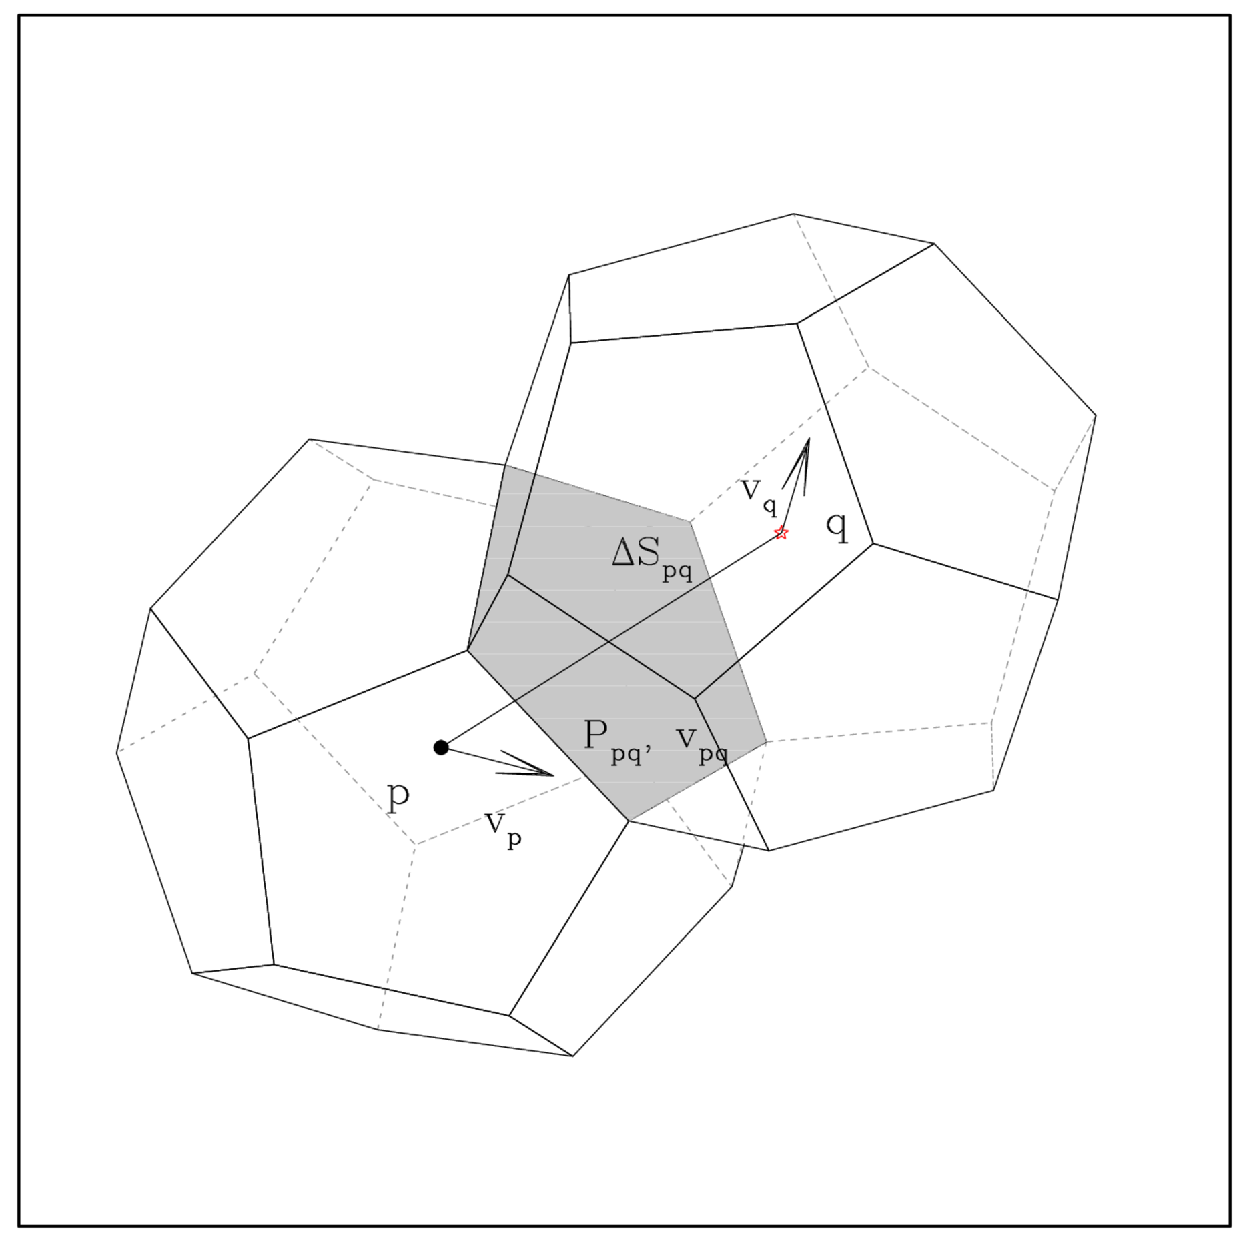
\includegraphics[width=\columnwidth]{3dneigh.pdf}	
\caption{Hydrodynamic interactions between two Laguerre cells. The Voronoi-neighboring, $p$ (filled circle) and $q$ (open star symbol), share the same interacting face (shaded in gray) with the surface vector $\Delta \surf_{pq}$, surface pressure $P_{pq}$ and the surface velocity $\boldsymbol{v}_{pq}$.}
\label{3dneigh}
\end{figure}

Hereafter, we call a Laguerre site a particle when it is related to the hydrodynamics.




\section{Discretizations of the Basic Conservation Rules}
We assume that the Laguerre cell is the Lagrangian control volume. Therefore, the mass conservation is self-evident because no mass flux is allowed through the Laguerre faces. Figure \ref{3dneigh} shows an example of Laguerre cells of a pair of neighboring particles $p$ and $q$. Their mutual contact surface is color coded in gray. The pressure and velocity on the surface face are labelled as $P_{pq}$ and $\boldsymbol{v}_{pq}$ which are the basic quantities in solving the hydrodynamic equations as shown below.


\subsection{Momentum Conservation}
The force on a Laguerre cell of the particle $p$ is the net force on the Laguerre-cell faces as
			\begin{eqnarray} \nonumber
				 {\boldsymbol{F}}_p &=& m_p {d\vel_p\over dt} = \mathcal{D}_t^\Omega(\rho_p u_p) \\
				 &=& -\oint_{\partial\Omega}\pressure(r) d\surf(r) = {-\sum_{q\in \mathbb{N}(p)} \pressure_{pq} \Delta \surf_{pq} }
				\label{eq:force}
			\end{eqnarray}
			where $\pressure_{pq}$ is the average pressure measured on the Voronoi face ($\Delta \surf_{pq}$) between $p$ and $q$ (see Fig. \ref{3dneigh}). Considering that $\pressure_{pq} = \pressure_{qp}$ but $\Delta \surf_{pq} = -\Delta \surf_{qp}$, we simply confirm the anti-commutative nature of the face force as 
			\begin{equation}
				\boldsymbol{F}_{pq} = -\boldsymbol{F}_{qp},
			\end{equation}
			which means that the momentum is conserved by the symmetric nature of the scheme.			
			
\subsection{Energy Conservation} 

The total energy of the Laguerre cell is decomposed into the kinetic and internal energies and the time derivatives of them are related as
\begin{equation}
				{dE_p\over dt} = {dT_p\over dt} + {dU_p\over dt}
\end{equation}
where $T$ and $U$ are the kinetic and internal energies. The change of the kinetic energy is obtained by multiplying equation (\ref{eq:force}) with the velocity of  $p$ as
\begin{eqnarray} 
			{dT_p\over dt} &\equiv& \boldsymbol{F}_p\cdot \vel_p= m_p {d\vel_p\over dt} \cdot \vel_p \\ &=&-\left(\oint_{\partial\Omega} \pressure(r) d\surf(r)\right) \cdot u = \sum_{q\in\mathbb{N}(p)} \pressure_{pq}\Delta \surf_{pq}\cdot \vel_p, 
\end{eqnarray}
where the last equation is the discretized sum over the polygon faces.
Likewise, the internal energy changes as
\begin{eqnarray}
				{d U_p \over dt} &=& -\oint_{\partial\Omega} \pressure(r) d \surf_{pq}(r) \cdot ( 
				\vel_{pq}^\textrm{rad}(r) - \vel_p )  \\
				&=& -\sum_{q\in\mathbb{N}(p)} \pressure_{pq} \Delta S_{pq} \cdot (\vel_{pq}^\textrm{rad} - \vel_p ),
\end{eqnarray}
where $\vel_{pq}^\textrm{rad}$ is the velocity of the Laguerre face, $\Delta \surf_{pq}$. Then, the volume increase over the face is $\Delta V = \surf_{pq}\cdot(\vel_{pq}^\textrm{rad}-\vel_p)$.


Finally, the  total energy would be expressed as
\begin{equation}
				{dE_{p}\over dt} = -\sum_{q\in\mathbb{N}(p)} \pressure_{pq}\Delta \surf_{pq}\cdot \vel_{pq}^\textrm{rad}. 
\end{equation}
In the calculations this face velocity is $\vel_{pq}^{\rm face}$ of equation~(\ref{eq:dEface}), which equals $\vel_{pq}^{\rm geo}$ on an ordinary face and carries the HLL normal speed only on an extreme face.
The change of total energy between $p$ and $q$ is anti-symmetric as
\begin{equation}
				{d \boldsymbol{E}_{pq}\over dt} \equiv - \pressure_{pq}\Delta \surf_{pq}\cdot\vel_{pq}^\textrm{rad} = -{d\boldsymbol{E}_{qp}\over dt}
\end{equation}
because $\vel_{pq} = \vel_{qp}$ and $\surf_{pq} = - \surf_{qp}$. This proves the conservation of total energy of the pair of Voronoi particles consequently.

			




\section{Tests of the geometric-face scheme}

GFS is the only scheme used in the tests of this section.
Every weight is zero.
An ordinary face takes the HLLC pressure and the geometric velocity of equation~(\ref{eq:vgeo}).
An extreme face takes the HLL state of equation~(\ref{eq:hll}).
The integrator is fourth-order Runge--Kutta.
An earlier comparison of five face algorithms on the same one-dimensional problems is given in Appendix~\ref{app:fivemethods}.


\subsection{Sod shock tube}

The Sod shock tube is the Riemann problem $(\rho,P,\vel)=(1,1,0)$ for $x<0.5$ and $(0.125,0.1,0)$ for $x\ge 0.5$, on $0\le x\le 1$, with reflecting walls.
Figure~\ref{fig:sodgfs} shows GFS at $N=200$.
The density $L_1$ is $5.86\times 10^{-3}$ and the energy error is $1.3\times 10^{-8}$.
The shock, the contact, and the rarefaction sit on the reference solution.

\begin{figure*}[htbp!]
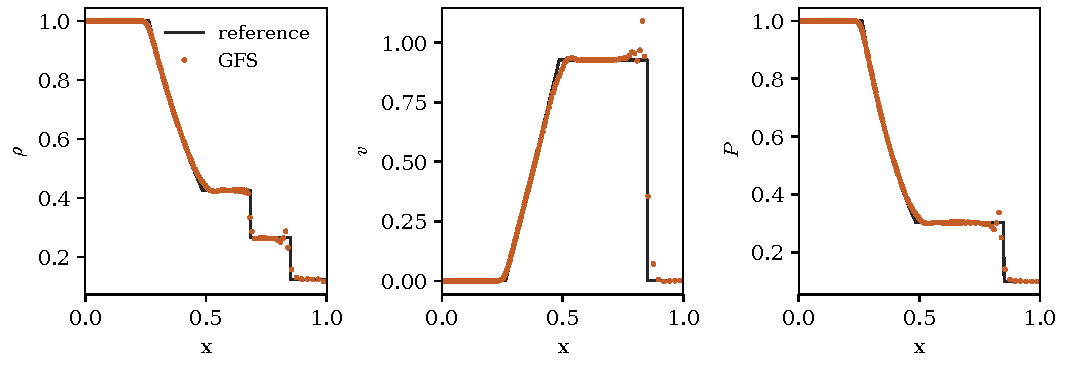
\includegraphics[width=\textwidth]{fig_sod.pdf}
\caption{Sod shock tube at the standard end time for GFS with $N=200$. The panels are density, velocity, and pressure. Points are particles and the line is the reference solution.}
\label{fig:sodgfs}
\end{figure*}

\subsection{One-dimensional problems}

Figure~\ref{fig:gfs1d} collects eight standard problems at $N=200$, except the Shu--Osher panel, which uses $N=800$.
Every run is GFS. Transmissive boundaries insert the exterior state when the velocity points into the domain.
The density $L_1$ values are $5.86\times10^{-3}$ (Sod), $0.154$ (blast), $1.36\times10^{-2}$ (Noh), $0.571$ (Shu--Osher), $5.25\times10^{-3}$ (Lax), $2.86\times10^{-2}$ (double rarefaction), $0.105$ (collision), and $6.48\times10^{-3}$ (contact).
The energy error is below $10^{-5}$ on every problem except the blast, where it is $3.3\times10^{-2}$.
In the Shu--Osher problem the left state has velocity $2.629$. The shock in the $N=800$ calculation lies at $x=2.39$, on the reference shock.

\begin{figure*}[htbp!]
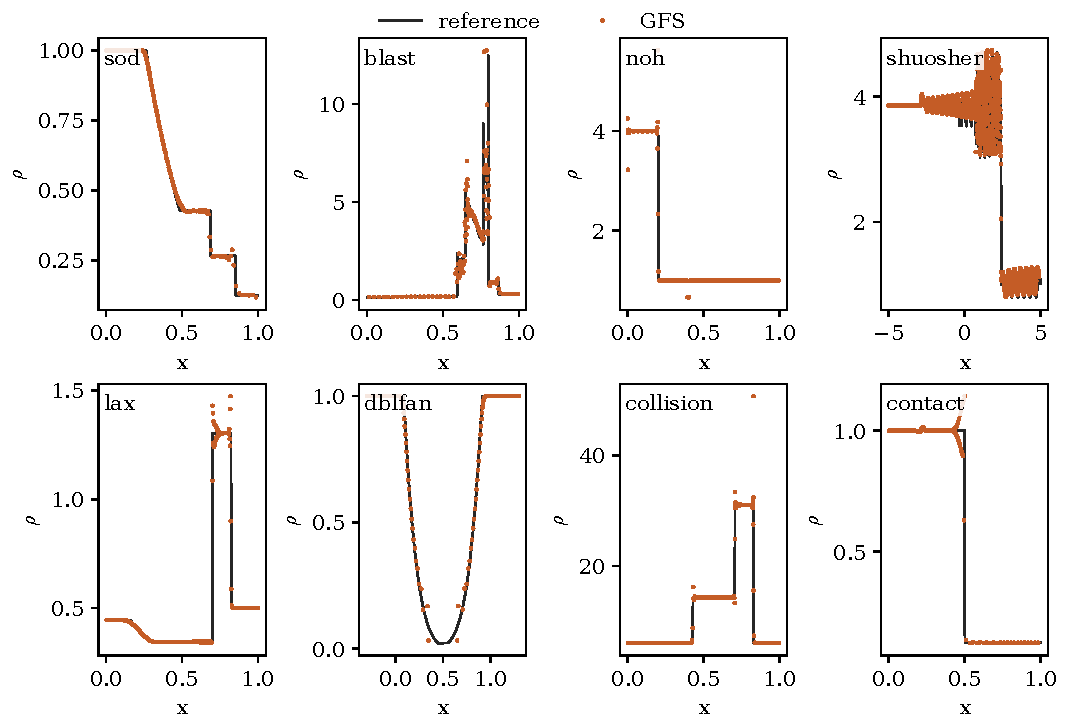
\includegraphics[width=\textwidth]{fig_gfs_1d.pdf}
\caption{GFS density for eight one-dimensional problems. Points are the particles and the line is the reference. $N=200$, except Shu--Osher, which uses $N=800$. The panel title names the problem.}
\label{fig:gfs1d}
\end{figure*}

\subsection{Gresho vortex}

The Gresho vortex is a stationary azimuthal flow on the unit square, with $\rho=1$ and a triangular $v_\phi(r)$ that peaks at $1$ when $r=0.2$.
Figure~\ref{fig:gresho} shows GFS at $t=1$ with $128\times128$ particles.
The mean absolute error in $v_\phi$ is $2.1\times10^{-2}$, and the energy error is $2\times10^{-8}$.

\begin{figure*}[htbp!]
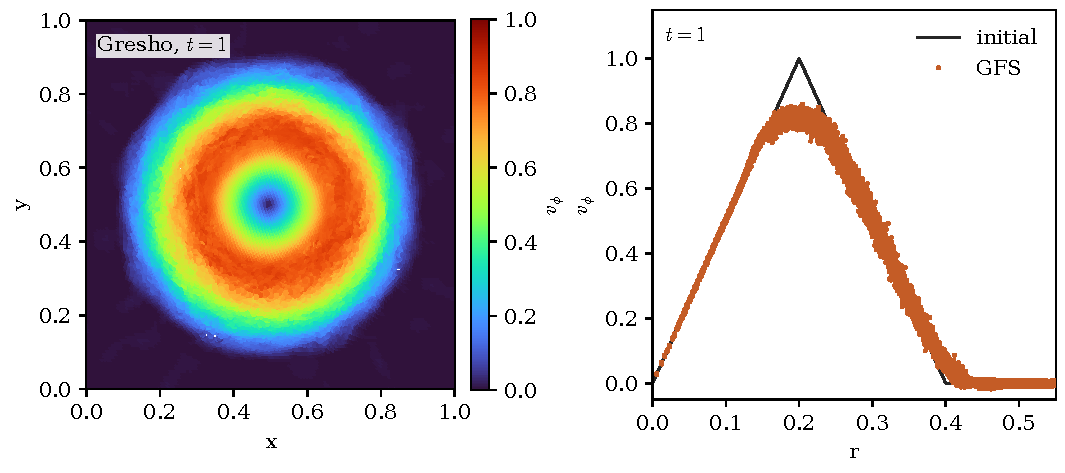
\includegraphics[width=\textwidth]{fig_gresho.pdf}
\caption{Gresho vortex with GFS at $t=1$. The left panel is $v_\phi$. The right panel compares the particles with the initial profile. The box is $0\le x,y\le 1$.}
\label{fig:gresho}
\end{figure*}

\subsection{KH Instability}

The Kelvin--Helmholtz calculation uses the shear layer of Lecoanet et al.\ on $0\le x\le 1$ and $0\le y\le 2$. The mesh contains $256\times512$ particles. Every weight is zero, and the face rule is that of Section~\ref{sec:adopted}. Figure~\ref{fig:kh} shows the layer from $t=0.5$ to $t=2$. The primary rolls are visible at $t=2$. The energy error is $3.7\times10^{-7}$. No internal energy is negative, and the kick does not clip it.

\begin{figure*}[htbp!]
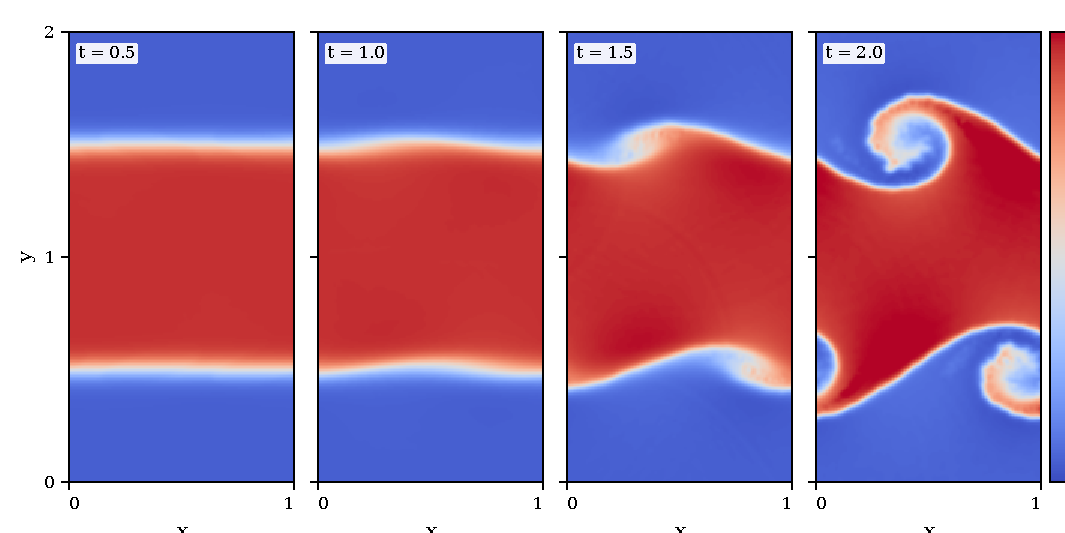
\includegraphics[width=\textwidth]{fig_kh.pdf}
\caption{Kelvin--Helmholtz density on $0\le x\le 1$, $0\le y\le 2$, with $256\times512$ particles and GFS. The shear layer rolls up between $t=0.5$ and $t=2$.}
\label{fig:kh}
\end{figure*}

\subsection{Rayleigh--Taylor instability}

The Rayleigh--Taylor calculation uses $256\times512$ particles on $0\le x\le 0.5$ and $0\le y\le 1$. The density ratio is $2$ and $g_y=-0.5$. The $y$ boundary is periodic, so the integration is stopped at $t=3$, before a spike can re-enter at $y=1$. Figure~\ref{fig:rt} shows the spikes. At $t=3$ the minimum $y$ of gas with $\rho>1.5$ is $0.227$. The energy error is $7.6\times10^{-4}$, and no internal energy is negative. A comparison calculation that assigned the Riemann contact speed to every face, including the shear faces along the spikes, increased the energy by a factor of $10^{7}$ by $t\simeq 2.2$.

\begin{figure*}[htbp!]
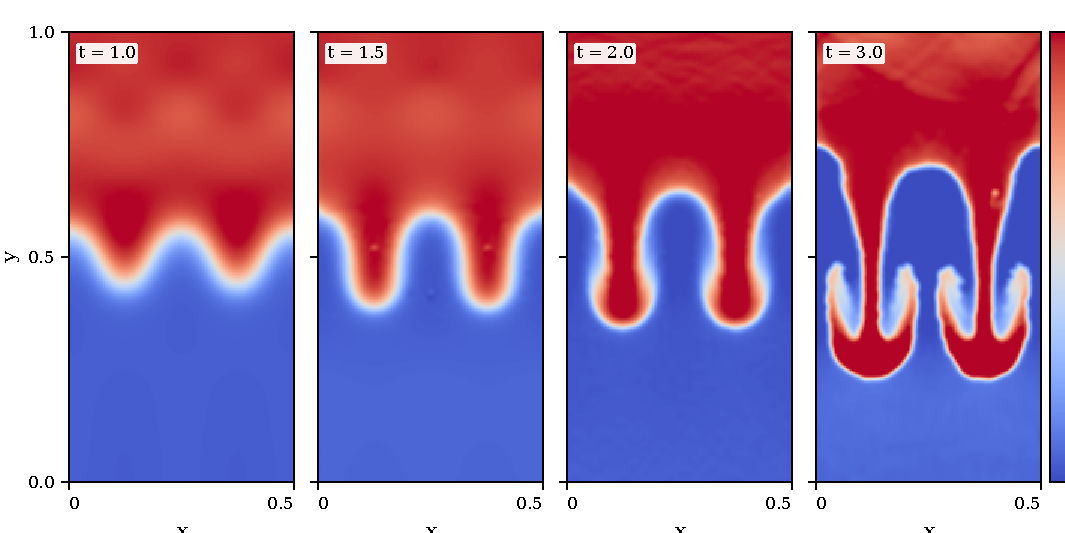
\includegraphics[width=\textwidth]{fig_rt.pdf}
\caption{Rayleigh--Taylor density with GFS and $256\times512$ particles. Heavy fluid is on top. At $t=3$ the lowest gas with $\rho>1.5$ is at $y=0.227$.}
\label{fig:rt}
\end{figure*}

\subsection{Mach-3 flow past a cylinder}

The Mach 3 stream has density $\rho=1$, velocity $\vel=1$, and pressure $P=0.08$. The sound speed is $\simeq 0.33$. The stream passes a solid cylinder of radius $R=0.5$ centred at $(2.5,\,2)$. Figure~\ref{fig:cyl} uses the domain $0\le x\le 20$ and $0\le y\le 4$ with $400\times 80$ particles, so the cell size is $0.05$. The wall is the reflecting ghost in equation~(\ref{eq:ghost}). At $t=5$ no particle lies inside the cylinder, and the smallest particle radius is $0.504$. The energy differs from its initial value by $-1.0\%$. The maximum density is $9.4$, and the time step is $\simeq 8\times 10^{-3}$. A previous integration that projected particles onto $r=R$ after each step reached $\rho_{\max}=635$ and an energy error of order $10^{7}$ by $t=2.58$. The black disk in the figure is the solid cylinder. The thin white edge is a plotting stroke that keeps the disk visible against the wake. The stroke is not a layer of absent gas.

\begin{figure*}[htbp!]
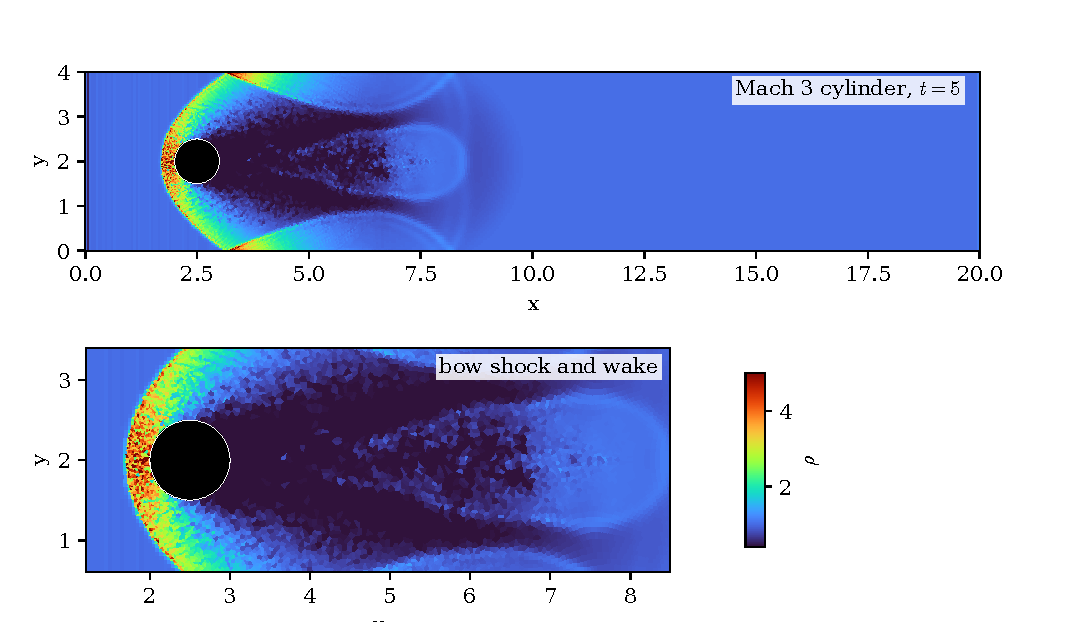
\includegraphics[width=\textwidth]{fig_cyl.pdf}
\caption{Mach-3 flow past a solid cylinder at $t=5$ on $0\le x\le 20$. The black disk is the cylinder. The bow shock stands upstream and the wake extends downstream. The colour scale runs from $0.4$ to $5$.}
\label{fig:cyl}
\end{figure*}

\subsection{Two-dimensional Noh problem}

Cold gas of density 1 and pressure $10^{-6}$ fills the unit square, and every particle moves toward the centre at speed 1. For $\gamma=5/3$ the shock stands at $r=t/3$. The density is 16 behind the shock and $1+t/r$ ahead of it.

Figure~\ref{fig:noh2d} shows GFS at $t=0.10$ with $64\times 64$ particles and zero weights. The median density in $r<0.05$ is 14.9. Ahead of the shock the binned median follows $1+t/r$. The energy error at this output is $5.2\times 10^{-3}$, and no internal energy is negative. The central density reaches 30. The cell size is comparable to the shock radius, so the post-shock plateau is carried by a few radial bins. Four particles that began at the corners of the square have cell volumes of 432. Their neighbour spacing is 0.93 cell widths and their weights are zero. The radial medians omit those four particles.

\begin{figure*}[htbp!]
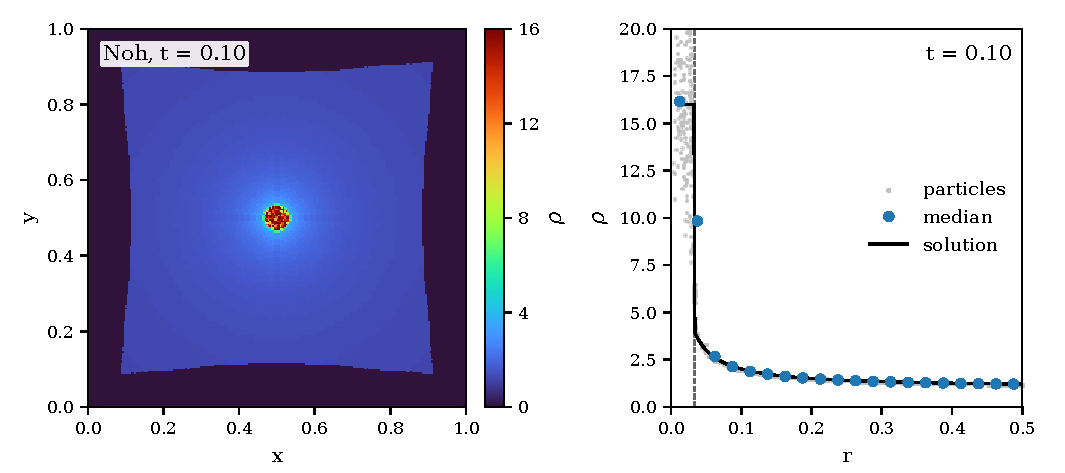
\includegraphics[width=\textwidth]{fig_noh2d.pdf}
\caption{Two-dimensional Noh problem with GFS at $t=0.10$. The left panel is density. The right panel compares the particles and their radial median with the solution. The dashed line is the shock radius $t/3$.}
\label{fig:noh2d}
\end{figure*}

\subsection{Keplerian ring}

A Gaussian ring of width 0.25 is centred at $R=1.5$ in a periodic square of side 4. The rotation is the softened Keplerian speed of a point mass $GM=1$ with softening $0.05$, and the scale height is $H/R=0.1$. The mesh has $128\times 128$ particles.

Figure~\ref{fig:kepler} follows the ring from $t=0.10$ to $t=1.00$. The five density panels use one colour scale. For gas with $\rho>0.2$ and $0.8<R<1.9$, the median radius moves from 1.53 to 1.55 and the radial standard deviation from 0.244 to 0.251. At $t=1.00$ the median of $v_\phi/v_K$ is 0.9994 and the mean absolute deviation from $v_K$ is $3.0\times 10^{-3}$. The energy error is $4.0\times 10^{-3}$. Twelve particles at $R=1.89$ lie below the Keplerian curve, with $v_\phi\simeq 0.63$.

\begin{figure*}[htbp!]
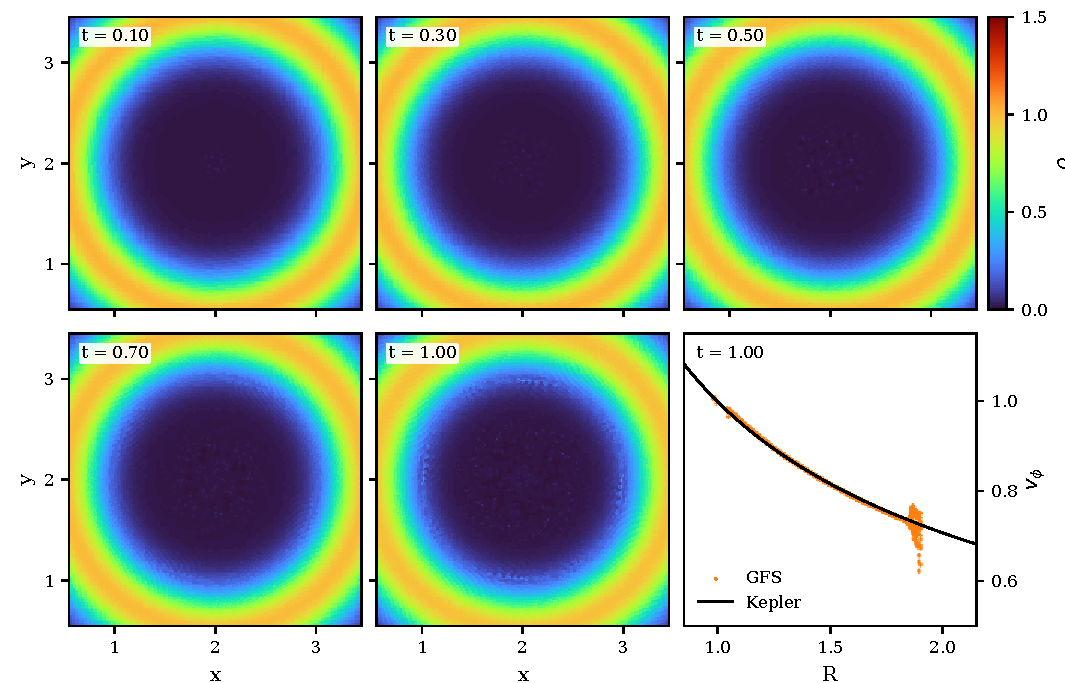
\includegraphics[width=\textwidth]{fig_kepler.pdf}
\caption{Keplerian ring with GFS. Density is shown at $t=0.10$, $0.30$, $0.50$, $0.70$, and $1.00$ on a common scale from 0 to 1.5. The bottom-right panel is $v_\phi$ at $t=1.00$ for $\rho>0.2$ against the softened Keplerian speed.}
\label{fig:kepler}
\end{figure*}

\section{Astrophysical Recipes}
\subsection{Gas Cooling and Heating}
\subsection{IMF of Stars}
\subsection{Stellar and SN feedbacks}
\subsection{Metallicity Enrichment}
\subsection{AGN Feedbacks}


\section{Discussion}



\acknowledgments

The authors thank the Korea Institute for Advanced Study for providing computing resources (KIAS Center for Advanced Computation Linux Cluster System) for this work. JK was supported by a KIAS Individual Grant (KG039603) via the Center for Advanced Computation at Korea Institute for Advanced Study. This work benefited from the outstanding support provided by the KISTI National Supercomputing Center and its Nurion Supercomputer through the Grand Challenge Program (KSC-2018-CHA-0003). Large data transfer was supported by KREONET, which is managed and operated by KISTI.


\appendix
\section{Weight tracers not used by GFS}
\subsection{How to Evolve the Power Distance}
To actively adjust in the site's {power distance} ($\omega$), we apply a model of the expansion or contraction of a gas cell to scale with the enthalpy as $\omega^2 \propto \mathcal{H}_i =mC_s^2/(\gamma-1)$. Therefore, the change of power distance is
\begin{equation}
	\Delta\omega^{i} \equiv \tilde\omega^{i+1}-\omega^{i} = \left[ \left( \frac{\mathcal{H}^{i}}{\left<\mathcal{H}^i\right>}\right)^{1/2} -1\right] \omega^{i},
\end{equation}
where $\left<\pressure^i\right>$ is defined as surface-averaged pressure of surrounding neighbors. It is noteworthy that during the IC setup, a separate scaling parameter, $\left<\omega\right> = \varkappa_\omega d_\textrm{mean}$, is introduced, typically initialized with $\varkappa_\omega=0.5$.

However, since the rate of power distance change ($v_p^\omega \equiv\Delta\omega_p/\Delta t)$ should not exceed the sound speed, the maximum expansion or contraction of the power distance per time step is constrained by 
\begin{equation}
	-c_s(p) \Delta t \le \Delta \omega_p \leq c_s(p) \Delta t
\end{equation}
where $c_s(p)$ is the sound speed and $\Delta t$ is the time step size. The value of power radius at step $i$ is, consequently, the minimum among the two corresponding values as
\begin{equation}
	\omega^i_p = \min \left( \tilde\omega^i_p, \omega_{p,\textrm{ceil}}^i\right).
\end{equation}


\subsection{Thermodynamic Tracers for the Power Distance}
\label{sec:w2modes}
The enthalpy-based model above treats the power distance as a response to
the local thermodynamic state. Because the Laguerre tessellation is
invariant under a rigid rescaling $\omega_p\to\omega_p+c$, what physically
controls the geometry is the \emph{variation} of~$\omega^2$ across the
flow, not its absolute value.  This invites a family of alternatives
differing only in the tracer functional $\Phi$ that is used to weight the
sites.  We implement three such options, all of the form
\begin{equation}
  \omega_p^2 = \varkappa_\omega^2\, d_\textrm{mean}^2 \; q_p, \qquad
  q_p = Q\!\left(\pressure_p,\rho_p\right),
  \label{omega_tracer}
\end{equation}
with $\varkappa_\omega\,d_\textrm{mean}$ setting the overall scale and
$Q$ a dimensionless profile.  The implemented tracers are:

\textit{(i) Pressure-based (default, \texttt{w2\_mode=0}).}
$Q = \left(\pressure_p/\pressure_0\right)^{\alpha_\omega}$ with
$\alpha_\omega=(\gamma-1)/\gamma$ and $\pressure_0$ a reference pressure
fixed by the IC.  At a subsonic contact discontinuity
($\pressure_p=\pressure_q$) this gives $\omega_p^2\approx\omega_q^2$, so
the radical axis coincides with the Voronoi bisector and cells across the
contact share a common size.  This is the choice that dissipates least at
material interfaces but carries no material tag.

\textit{(ii) Entropy-A power law (\texttt{w2\_mode=1}).}
$Q = \left(A_p/A_\textrm{ref}\right)^{\alpha_\omega}$ with the entropic
function $A_p\equiv \pressure_p/\rho_p^{\gamma}$ and
$A_\textrm{ref}=\pressure_0/\rho_\textrm{ref}^{\gamma}$ (geometric-mean
density in the IC).  In smooth adiabatic flow $A_p$ is conserved along
streamlines, so $\omega_p$ is constant within each fluid but jumps across
contacts by $(\rho_q/\rho_p)^{\alpha_\omega\gamma}$.  Cells of different
materials therefore have geometrically distinct sizes---a useful tag,
but the contact acquires a face-area asymmetry that can bias the flux
calculation when $\alpha_\omega$ is large.

\textit{(iii) Specific-entropy additive (\texttt{w2\_mode=2}).}
$Q = 1 + \beta\,(s_p - s_\textrm{ref})/s_\textrm{scale}$, where
$s_p\equiv c_v\ln(\pressure_p/\rho_p^{\gamma})$ is the specific entropy
(up to the constant $c_v$, which cancels through
$s_\textrm{scale}$),
$s_\textrm{scale}=|s_1-s_2|=\gamma|\ln(\rho_1/\rho_2)|$ is a scale set by
the IC contact jump, and $\beta\in[0,1)$ is a dimensionless amplitude.
Unlike (ii), this tracer is \emph{linear} in $s$ and bounded: the
perturbation to $\omega^2$ is bounded by $\beta$ and so is the contact
jump in cell size.  The advective stability of $s$ in smooth flow means
the noise feedback $\delta\rho\to\delta A\to\delta\omega\to\delta\rho$
is damped both logarithmically (through $s = c_v\ln A$) and linearly
(through $\beta$), making small-$\beta$ runs safe against the
feedback-driven cell shrinkage that can plague (ii).
With the Kelvin--Helmholtz IC ($\rho_1=1$, $\rho_2=2$, $\gamma=5/3$), for example,
$s_\textrm{scale}=\gamma\ln 2\approx 1.155$ and $\beta=0.15$ produces an
$\approx\!11\%$ contrast in~$\omega^2$ across the contact, strong enough
to retain material identity while remaining within the
linear-perturbation regime.

For all three tracers the time-step safeguard of equation~(\ref{drad})
applies unchanged, and the ceiling $\omega_{p,\textrm{ceil}}$ together
with the optional relaxation, rate, and floor limiters
($\tau_\omega,\,r_\omega,\,\omega_\textrm{floor}$) act identically on the
resulting~$q_p$.  The choice of tracer therefore controls only the
functional form, not the admissible range, of the Laguerre weight.


\section{Face algorithms not used by GFS}
The algorithms in this appendix were implemented and compared during the development of the code. They are not part of GFS.

\section{Face-averaged Interpolations}
\subsection{A Relation between Cell-Averaged and Face-Averaged values}
First, we use the well-designed interpolation to get the average surface value from the corresponding Voronoi sites as
\begin{equation}
	\left< \phi\right>_\textrm{face}\equiv {1\over \partial \Omega(\mathbb{N}_n)}\int_{\partial \Omega(\mathbb{N}_n)} \phi dS   = \sum_{i\in \mathbb{N}_n} w_i\left<\phi_i\right>_\textrm{cell}
\end{equation}
where $\mathbb{N}_n$ is the  Voronoi sites shaping the face of interest and $w_i$ is the corresponding weighting.
Then, according to the Gauss theorem, we may get the spatial difference of $\phi$ from the surface integral as,
\begin{equation} \label{surface}
	\left<\nabla\phi\right>_\textrm{cell} = {1\over \Omega_\textrm{cell}} \oint_{\partial \Omega} \phi dS  = {1\over \Omega_\textrm{cell}}\sum_\textrm{face} \left<\phi\right>_\textrm{face} \Delta S_\textrm{face}
\end{equation}
where $\left<\phi\right>_\textrm{face}$ is the averaged value on the face element, $\Delta S_\textrm{face}$, and $\Omega_\textrm{cell}$ is the cell volume.

To summarize, equation (\ref{looping}) shows how the derivatives of the cell-averaged value are obtained by applying the recursive loop. \begin{eqnarray} \nonumber \label{looping}
	\left<\phi\right>_\textrm{cell} &\rightarrow &\left<\phi\right>_\textrm{face} \Rightarrow \left<\nabla\phi\right>_\textrm{cell} \rightarrow \\ \nonumber &\rightarrow& \left<\nabla\phi\right>_\textrm{face} \Rightarrow \left<\nabla^2\phi\right>_\textrm{cell} \rightarrow \\ 
	&\rightarrow& \left<\nabla^2\phi\right>_\textrm{face} \Rightarrow \left<\nabla^3\phi\right>_\textrm{cell} \rightarrow \cdots
\end{eqnarray}
where $\Rightarrow$ means the cell-to-face interpolation and $\rightarrow$ means applying of the surface integral (eq. \ref{surface}). In the next subsequent sections, we will show how to compute those values in detail.





\subsection{Effects of the Simple Averaging Scheme}	
A hydro quantity ($\phi$) on the cell center is used to get the face-centered value on a Laguerre surface. For example, the second-order accuracy between $p$ and $q$ is simply given as,
\begin{equation} \label{secondorder}
	\phi_{pq} = {1\over2} \left( \phi_p + \phi_q\right),
\end{equation}
which  satisfies the symmetry of $\phi_{pq} = \phi_{qp}$. 
		
If we simply adopt the average velocity on the Laguerre face as $\vel_{pq} = {1\over2} (\vel_p + \vel_q)$, we may get a simple relation as
\begin{eqnarray}
	{dU_p\over dt} &=& -{1\over2}\sum_{q\in\mathbb{N}(p)} \pressure_{pq}\Delta \surf_{pq}\cdot (\vel_q - \vel_p) \\
	&=& -{1\over2}\sum_{q\in\mathbb{N}(p)} \Delta U_{pq},
\end{eqnarray}
which is symmetric between $p$ and $q$. Therefore, it implies that the change of internal energy is same between the Laguerre pair ($\Delta U_{pq} = \Delta U_{qp}$).
Also another intriguing property can be obtained when the pressure on the Laguerre faces are averaged as $P_{pq}=(P_p+P_q)/2$ and, then, we may obtain from equation (\ref{eq:force}) as
\begin{equation} \label{eq:netforce}
				F_p = - \sum_{q\in\mathbb{N}(p)}\left({\pressure_q\over2}\right) \Delta \surf_{pq}
\end{equation}
where we have used the relation $ \sum_q \Delta \surf_{pq} = 0$. From this result, we may know that the force on the target particle is completely determined by the pressure of its Laguerre neighbors.

\subsection{Generalization of the Face-Centered Approximation}
For the higher-order generalization, we adopt the functional form of equation (\ref{secondorder}) as
\begin{equation}
	\phi_{pq} = \sum_{s\in\mathbb{N}(p)}{W}_{pq}^s {\phi}_{s}
\end{equation}
where ${\phi}_{s}$ is the cell-centered hydro quantity (pressure or velocity) of the neighbor, $s$, which may have a contribution to forming the Voronoi surface, $\Delta\surf_{pq}$.


The weighting for the neighboring particles is expressed into $m$-dimensional vector as
\begin{equation}
	\boldsymbol{W}_{pq} \equiv (w_p, w_q, w_{r}\cdots, w_{r+m-3})
\end{equation}
where the first element is the contribution from the target site, the second one is from the facing neighbor, and the remains are contributions from the other neighbors.
For the conservation of momentum and energy, we have to set $w_p = w_q$ and $w_r = \cdots = w_{r+m-3}$.


\subsection{Weighting on One-Dimensional Surface}
In the 2-dimensional space, the weighting vector should have four components because to make a Laguerre surface we need three neighboring sites beside the target site (see Fig. \ref{octagon2d}). Below, we show two exemplary cases for the two-dimensional weighting vector; 
\begin{eqnarray}
	\boldsymbol{W}^\text{2D}_\text{2nd} &=& \left({1\over2},{1\over2},0,0\right) \\
	\boldsymbol{W}^\text{2D}_\text{LP} &=& \left({4\over9},{4\over9},{1\over 18}, {1\over 18}\right), 
\end{eqnarray}
where the first one has the second-order accuracy while the last one has the fourth-order accuracy \citep{LILEK1995239}. Figure \ref{octagon2d} depicts how to formulate the weighting of the contributions of neighbors in 2-D. As the central node on the 2-D Laguerre face is equidistant from $p$ and $q$, we may set $\phi_c = (\phi_p +\phi_q)/2$. Likewise, for the left- and right-end nodes of the Laguerre surface, we set $\phi_1 = (\phi_p+\phi_q+\phi_s)/3$ and $\phi_2 = (\phi_p+\phi_q+\phi_r)/3$, respectively because the end node is equidistant from those three sites. We can get the average value on the Laguerre face as 
\begin{eqnarray}
	\overline{\phi} &=& \left(1-{2}\omega\right)\phi_c + {\omega}\phi_\text{l} + {\omega}\phi_\text{r}\\
	&=&  \left({1\over2}-{\omega\over3}\right)(\phi_p+\phi_q) + {\omega\over3}(\phi_r+\phi_s) 
\end{eqnarray}
where  $\omega$ is the weighting of the edge node, and it should have a range as $0\le \omega\le 1/2$. If the edge nodes have a null contribution to the average value on the 2-D Laguerre face, then we may set $\omega=0$ and this is the case for $\boldsymbol{W}_\text{2nd}^\text{2D}$. For $\boldsymbol{W}_\text{LP}^{2D}$, we get $\omega=1/6$.  See \ref{baryinter} for the affine combination of nodes with the homogeneous interpolation on the line.


\begin{figure}[t!] 
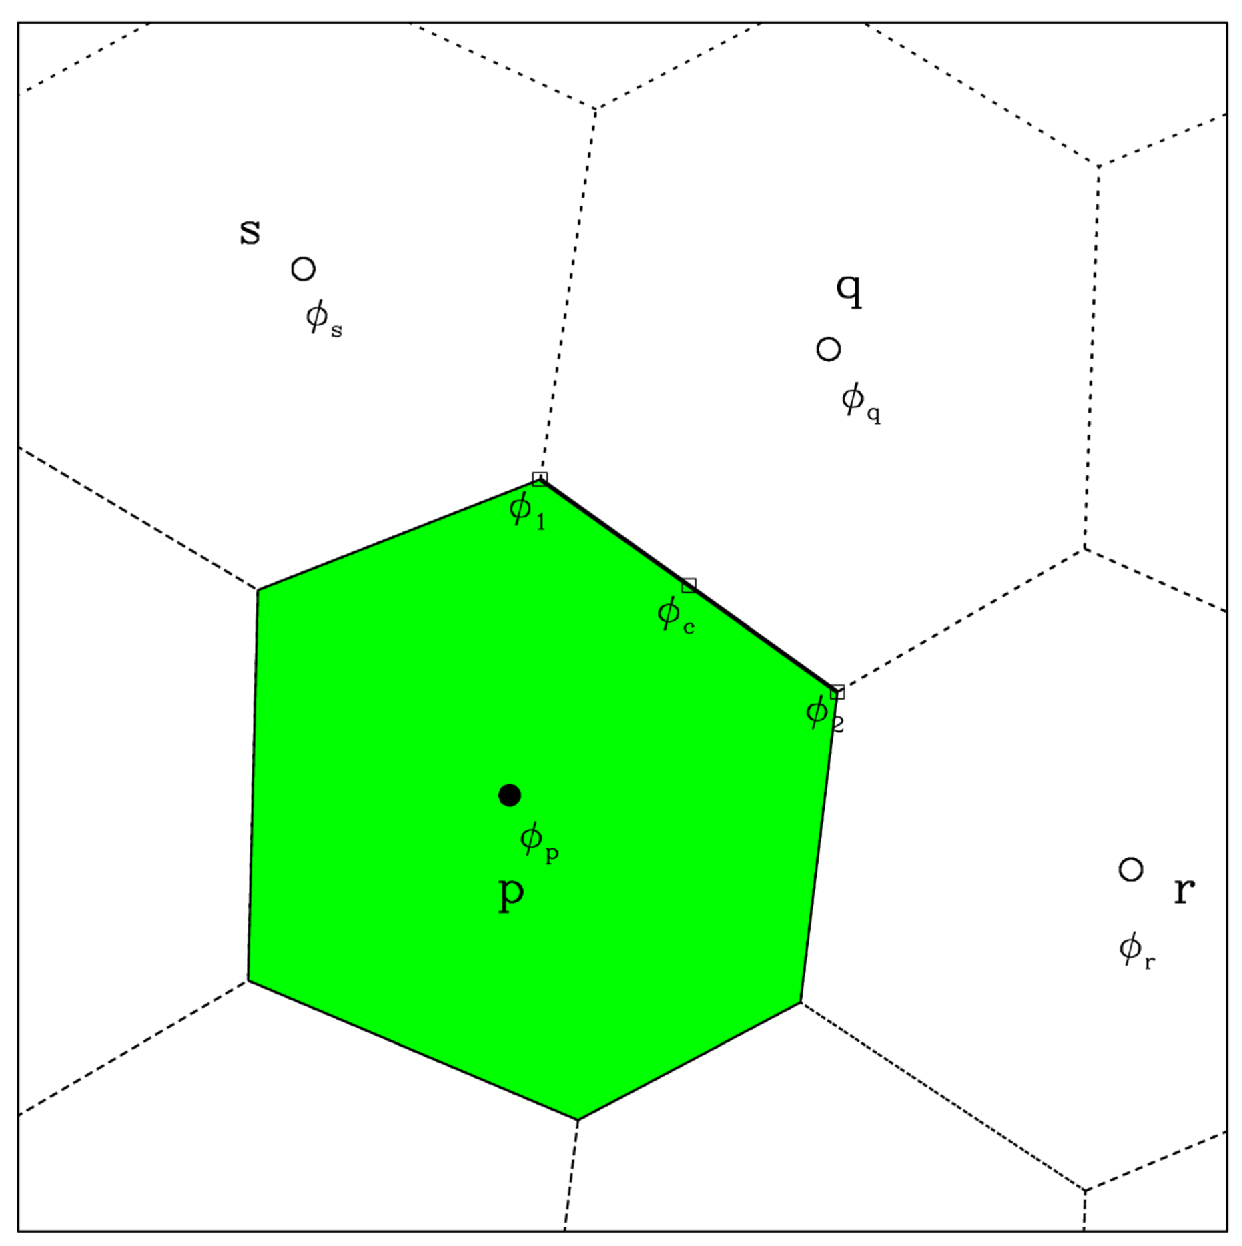
\includegraphics[width=\columnwidth]{octagon2d.pdf}	
\caption{Illustration of two-dimensional weighting scheme. The target site ($p$) marked with the filled circle has a cell color-coded with green. Three neighboring sites ($q$, $r$, and $s$) marked with open circles forms the Laguerre face (thick line). Here we mark the central and left-/right-end nodes of the Laguerre face with the open squares. The values of $\phi$ on the face are denoted as $\phi_1$, $\phi_c$, and $\phi_2$, from the left.}
\label{octagon2d}
\end{figure}


\subsection{Weighting on Two-Dimensional Surface}
On the two-dimensional surface, the situation becomes more complex, but it can be managed by decomposing the Laguerre face into multiple triangles. Since the Laguerre face forms a convex polygon in 3-D, we may find the barycenter of the polygon and interpolate values within each triangle. 

\texttt{https://www.inf.usi.ch/hormann/papers/Hormann.2014.BI.pdf}

\texttt{Mean Value Coordinates for Arbitrary Planar Polygons
KAI HORMANN
Clausthal University of Technology}

To illustrate the adopted weighting process, we present Figure \ref{3dface}. First, in panel (a), the Laguerre face is highlighted in gray. This face is a pentagon, with its barycenter indicated by the symbol O in panel (c). The pentagon is tessellated into five triangles, all sharing the barycenter as a common vertex. A shear mapping is applied to each triangle to transform them to right triangles, as shown in the transition from panel (c) to panel (d).
\begin{figure}[t!] 
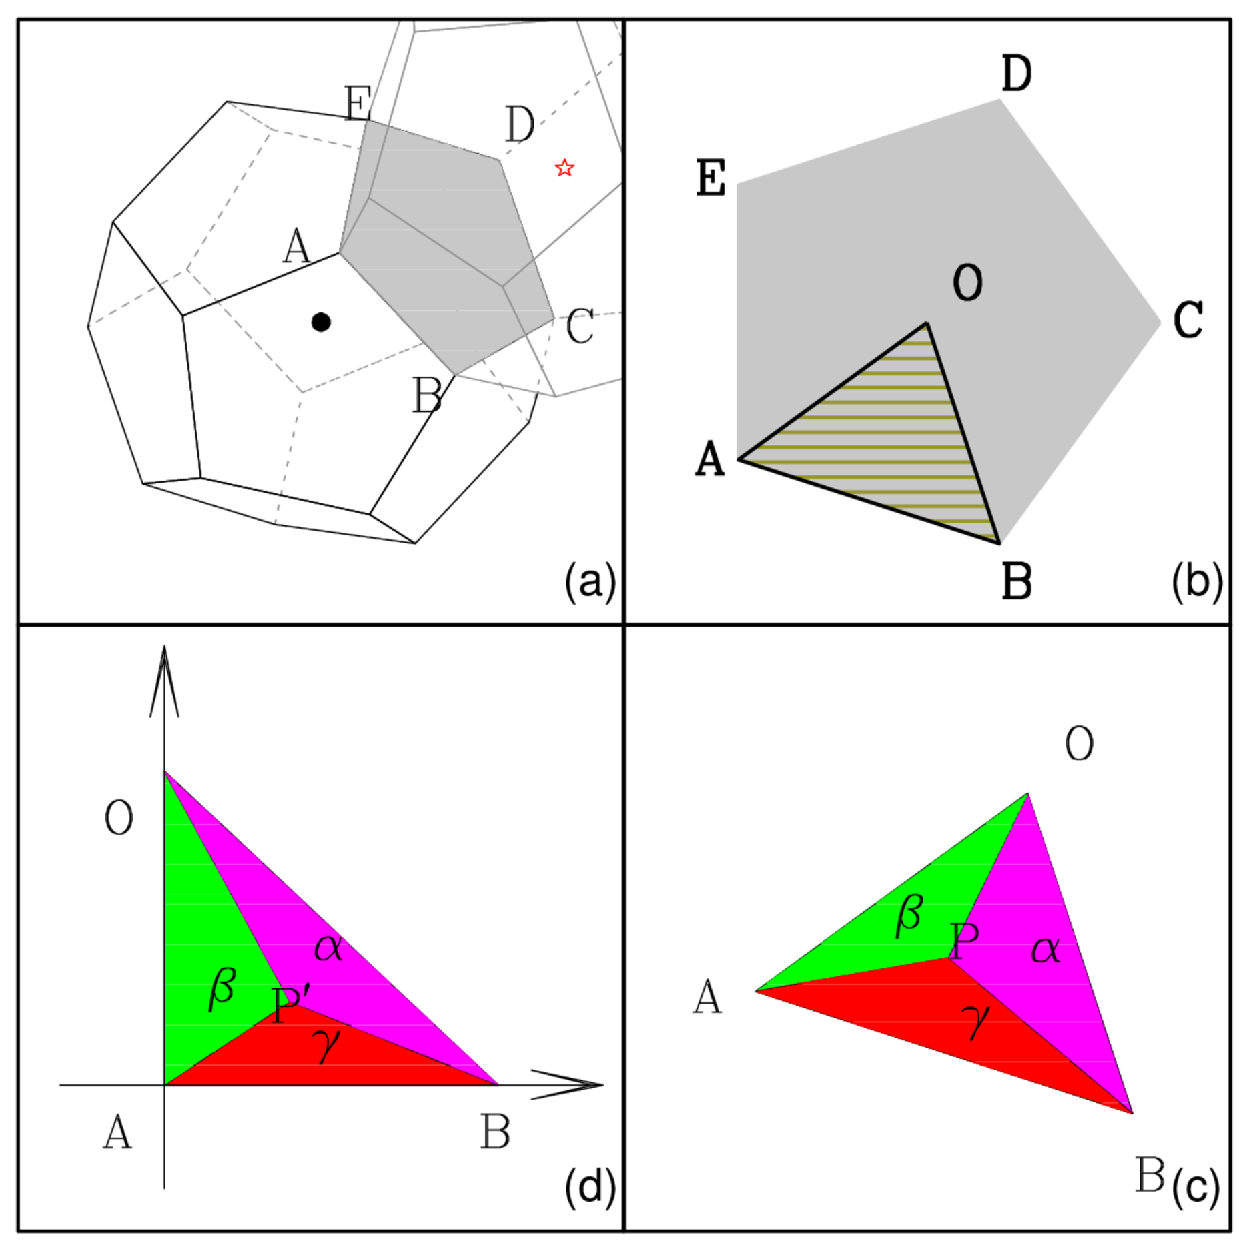
\includegraphics[width=\columnwidth]{3dface.pdf}	
\caption{Illustration of the three-dimensional weighting scheme. Our approach for determining the average value on the Laguerre surface (represented as a gray pentagon) is depicted in a counterclockwise sequence, beginning from the top-left panel. (a) Two Laguerre cells are shown, with the shared Laguerre face highlighted in gray. (b) The Laguerre surface is decomposed into multiple triangles, and one example triangle is shown. (c) With the arbitrary inner point $P$, the triangle is further tessellated with three subtriangles with areas, $\alpha$, $\beta$, and $\gamma$, which are called the barycenter coordinate of $P$ after normalization. (d): Through a proper shear mapping, the triangle can be transformed to a right triangle. In this mapping, the area is preserved and straight lines remain straight.}
\label{3dface}
\end{figure}



According to the model of two-dimensional univariate barycentric interpolation, we define values at arbitrary positions inside the triangle as
 \begin{equation}
 	\phi(x,y) \equiv {\alpha\phi_A +\beta\phi_B+\gamma\phi_O \over\alpha+\beta+\gamma}
 \end{equation}
 where $\alpha$, $\beta$, and $\gamma$ are the surface areas of subtriangles corresponding to their vertices (see panel (c)). The normalized terms of them are often called the barycentric coordinate for $(x,y)$. Then, for example, the contribution of the vertex $A$ to the point $(x,y)$ is proportional to the area of subtriangle, $\alpha$.
 
 On the other hand, after the shear mapping as show in panel (d), we are able to measure the average value on the triangle as 
 \begin{eqnarray}
 	\overline{\phi}_{\Delta ABO} &=& \int_{\Delta ABO}P(x,y)dxdy \\ \label{onethird}
 	&=& {1\over3}\left( \phi_O +\phi_A + \phi_B\right).
 \end{eqnarray}
which simply implies that the average value on the triangle is a simple average of values defined at the vertices.
While the value at the barycenter is determined by the two sites as $\phi_O = (\phi_p+\phi_q)/2$, the values at the other two nodes are averaged by additional neighbors as
\begin{eqnarray}
	\phi_A &=& {1\over 4}\left(\phi_p +\phi_q + \phi_r + \phi_s \right) \\
	\phi_B &=& {1\over 4}\left(\phi_p +\phi_q + \phi_t + \phi_u \right).
\end{eqnarray}
From now on, rather than using equation (\ref{onethird}), we adapt the relative weighting of nodes as
\begin{eqnarray}
	\overline{\phi}_{\Delta ABO} &=& \left( 1 - {2\omega}\right) \phi_O + {\omega} \phi_A + {\omega} \phi_B \\ \nonumber
	&=& \left( {1\over2} - {\omega\over2}\right) \left( \phi_p + \phi_q\right) + {\omega\over 4}\left( \phi_r +\cdots +\phi_u\right)
\end{eqnarray}
For $\omega=1/3$, we may get the weighting vector on the triangle as
\begin{eqnarray}
	\boldsymbol{W}^\text{3D}_\text{JK} &=& \left({1\over3},{1\over3},{1\over 12}, {1\over 12}, {1\over 12}, {1\over 12}\right)
\end{eqnarray}

Finally, the surface-weighted average of $\phi$ on the tessellated triangles is obtained as
\begin{equation*}
	\left<\phi\right>_\text{VF} = { \sum_i S(\Delta_i)\overline{\phi}_i \over \sum_i S(\Delta_i)}
\end{equation*}
where $S(\Delta_i)$ is the area of the $i$'th tessellated triangle and $\overline{\phi}_i$ is the average $\phi$ on the triangle.


\subsection{Face-Averaged Viscous Stress}
\label{sec:facetau}

The Navier--Stokes viscous stress tensor established
in Section~2 (eq.~\ref{eq:tau}) can be naturally
incorporated into the M$(n,m)$ face-pressure framework
without additional machinery.
The cell-averaged velocity gradient tensor is already
available from Section~2.8:
\begin{equation}\label{eq:gradv_cell}
  \left<\gradT{u}\right>_p
  = \frac{1}{\Omega_p}
    \sum_{q\in\mathbb{N}(p)}
      \vel_{pq}\otimes\Delta\surf_{pq},
\end{equation}
together with the cell-averaged divergence
\begin{equation}\label{eq:divv_cell}
  \left<\nabla\!\cdot\!\vel\right>_p
  = \frac{1}{\Omega_p}
    \sum_{q\in\mathbb{N}(p)}
      \vel_{pq}\cdot\Delta\surf_{pq},
\end{equation}
where $\vel_{pq}$ is the face-averaged velocity from
the M$(n,m)$ interpolation of Section~5.3.

The cell-averaged viscous stress tensor follows directly:
\begin{equation}\label{eq:tau_cell}
  \left<\boldsymbol{\tau}\right>_p
  = -\nu_p\rho_p\left(
    \left<\gradT{u}\right>_p
    + \left<\gradT{u}\right>_p^\mathsf{T}
    - \tfrac{2}{3}\boldsymbol{I}\,
      \left<\nabla\!\cdot\!\vel\right>_p
  \right).
\end{equation}
The face-averaged viscous stress is obtained via the
same M$(n,m)$ weighting used for pressure and velocity:
\begin{equation}\label{eq:tau_face}
  \left<\boldsymbol{\tau}\right>_{pq}
  = \sum_{s} W^s_{pq}\,
    \left<\boldsymbol{\tau}\right>_s,
\end{equation}
inheriting the symmetry
$\left<\boldsymbol{\tau}\right>_{pq}
 = \left<\boldsymbol{\tau}\right>_{qp}$
from the M$(n,m)$ weights.

The momentum equation~(\ref{eq:force}) generalizes to
\begin{equation}\label{eq:mom_tau}
  m_p\frac{d\vel_p}{dt}
  = -\sum_{q\in\mathbb{N}(p)}
    \left(
      \left<\pressure\right>_{pq}\boldsymbol{I}
      + \left<\boldsymbol{\tau}\right>_{pq}
    \right)\cdot\Delta\surf_{pq},
\end{equation}
and the scalar viscous pressure (normal component)
relevant for the face force is
\begin{equation}\label{eq:pi_tau}
  \Pi_{pq}^{\tau}
  = \hat{n}_{pq}\cdot
    \left<\boldsymbol{\tau}\right>_{pq}
    \cdot\hat{n}_{pq}.
\end{equation}

\paragraph{Physical and artificial viscosity.}
The kinematic viscosity~$\nu_p$ in
equation~(\ref{eq:tau_cell}) admits two interpretations.
For physical (molecular) viscosity, $\nu$ is a constant
determined by the Reynolds number of the flow.
For shock capturing, $\nu_p$ is promoted to a
cell-dependent artificial viscosity:
\begin{equation}\label{eq:nu_av}
  \nu_p = \alpha_p\,h_p\,c_p,
\end{equation}
where $h_p = (\Omega_p)^{1/d}$ is the effective cell size,
$c_p$ is the sound speed, and $\alpha_p$ is the viscosity
coefficient.
With constant~$\alpha$ this recovers the classical
Monaghan-type artificial viscosity;
with the time-dependent CD10 switch
(Section~6.5, eqs.~\ref{eq:alphaloc}--\ref{eq:alphacd}),
the stress tensor adapts automatically to shocks.

\paragraph{Connection to signal-velocity AV.}
In one dimension with uniform spacing
$\Delta x \approx h$, the NS stress tensor reduces to
$\tau \approx -\alpha h c\,\rho\,(2\,\partial\vel/\partial x)$.
Comparing with the Price signal-velocity AV,
$\Pi = \tfrac{1}{2}\alpha\,v_\mathrm{sig}\,
  \bar\rho\,\Delta\vel$,
and noting $v_\mathrm{sig} \approx 2c$ for weak waves,
both expressions scale as $\alpha c\rho\Delta\vel$.
The NS form is the natural tensorial generalization,
correctly distinguishing shear from compression in
multiple dimensions.





\subsection{Time Steps}
The hydrodynamic time step is determined from the sound speed and the radial velocity as
\begin{equation}
	\Delta t_{pq} = 2 \mathcal{C}_\text{cfl} \left( {  \|\boldsymbol{r}_{pq}\| \over  v_\text{sig}}\right)
\end{equation}
where $v_\text{sig}\equiv \left(c^s_p+c^s_q - \min(0, \vel_{pq}\cdot e_{pq}) \right)$ and $\mathcal{C}_\text{cfl}$ is the Courant number. Finally, the global time step is determined as
\begin{equation}
	\Delta t = \min_p ( \min_{q\in\mathbb{N}(p)} (\Delta t_{pq}))
\end{equation}

For the fourth-order Runge-Kupta integration, we set $c_\textrm{cfl}=0.2$ while we use $c_\textrm{cfl}=0.1$ for the Leap-frog scheme.




\section{The HLLC + Cullen--Dehnen Scheme on 3D Laguerre Cells}
\label{sec:hllc3d}

\subsection{Motivation}

A simple artificial viscosity employs a fixed pair of
parameters $(\alpha,\beta)$ applied uniformly to every face.
While adequate for moderate shocks, this global prescription
over-dissipates smooth flows and under-resolves contact
discontinuities.
We therefore introduce a Riemann-solver--based face pressure
combined with a time-dependent viscosity switch, both validated
in one dimension (\ref{app:hllccd}).
This section describes how the algorithm maps onto the
cell-averaged / face-averaged framework established in Sections~4
and~5.

In this framework every hydrodynamic quantity is either a
cell-averaged value
$\left<\phi\right>_\textrm{cell}$, volume-integrated over the
Lagrangian cell~$\Omega_p$, or a face-averaged value
$\left<\phi\right>_\textrm{face}$, area-integrated over the
Laguerre face~$\partial\Omega_{pq}$.
The recursive loop of equation~(\ref{looping}) connects the two:
\begin{equation*}
  \left<\phi\right>_\textrm{cell}
    \;\xrightarrow{\text{interpolation}}\;
  \left<\phi\right>_\textrm{face}
    \;\xRightarrow{\text{surface integral}}\;
  \left<\nabla\phi\right>_\textrm{cell}.
\end{equation*}
The HLLC+CD10 scheme replaces the interpolation step
($\rightarrow$) for the pressure and normal velocity
with a Riemann-solver--based procedure, while the
surface-integral step ($\Rightarrow$) and the
M$(n,m)$ weighting for tangential quantities remain unchanged.


\subsection{Cell-Averaged Gradient via the Green--Gauss Theorem}

The starting point is the cell-averaged gradient already
established in equation~(\ref{surface}):
\begin{equation}\label{eq:gg}
  \left<\nabla\phi\right>_p
  = \frac{1}{\Omega_p}
    \sum_{q\in\mathbb{N}(p)}
      \left<\phi\right>_{pq}\,\Delta\surf_{pq},
\end{equation}
where $\left<\phi\right>_{pq}$ is the face-averaged value on
$\partial\Omega_{pq}$.
For the initial gradient estimate we use the second-order
face average of equation~(\ref{secondorder}),
$\left<\phi\right>_{pq} = (\left<\phi\right>_p + \left<\phi\right>_q)/2$,
so that equation~(\ref{eq:gg}) becomes
\begin{equation}\label{eq:gg2}
  \left<\nabla\phi\right>_p
  = \frac{1}{2\Omega_p}
    \sum_{q\in\mathbb{N}(p)}
      \bigl(\left<\phi\right>_q - \left<\phi\right>_p\bigr)
      \Delta\surf_{pq},
\end{equation}
where we used the closure relation
$\sum_q \Delta\surf_{pq} = 0$.
This is identical to the cell-averaged velocity gradient
of Section~2.8 and constitutes the first step of the
recursive loop~(\ref{looping}).

Equation~(\ref{eq:gg2}) is applied to $\phi \in \{P,\,\rho,\,\vel\}$
to obtain the cell-averaged gradients
$\left<\nabla P\right>_p$,
$\left<\nabla\rho\right>_p$, and
$\left<\nabla\vel\right>_p$.


\subsection{Slope Limiter for Cell-Averaged Gradients}

The unlimited gradient~(\ref{eq:gg2}) can create new extrema
when extrapolated to face centroids.
To enforce monotonicity we apply the Barth--Jespersen limiter
\citep{barth1989}.
For each cell~$p$, define the extrapolated increment toward face~$pq$:
\begin{equation}
  \delta\phi_{pq}
  = \left<\nabla\phi\right>_p \cdot
    (\vect{x}_{f,pq} - \vect{x}_p),
\end{equation}
where $\vect{x}_{f,pq}$ is the area-weighted centroid of the
Laguerre face~$\partial\Omega_{pq}$ and $\vect{x}_p$ is the
cell centroid.
The neighborhood extrema are
\begin{equation}
  \phi_{\max} = \max_{q\in\mathbb{N}(p)\cup\{p\}}
    \left<\phi\right>_q, \qquad
  \phi_{\min} = \min_{q\in\mathbb{N}(p)\cup\{p\}}
    \left<\phi\right>_q.
\end{equation}
The per-face limiter value is
\begin{equation}
  \Phi_{pq} = \begin{cases}
    \min\!\left(1,\;
      \dfrac{\phi_{\max} - \left<\phi\right>_p}
            {\delta\phi_{pq}}\right),
      & \delta\phi_{pq} > 0, \\[8pt]
    \min\!\left(1,\;
      \dfrac{\phi_{\min} - \left<\phi\right>_p}
            {\delta\phi_{pq}}\right),
      & \delta\phi_{pq} < 0, \\[8pt]
    1, & \delta\phi_{pq} = 0,
  \end{cases}
\end{equation}
and the cell limiter is
$\Phi_p = \min_{q\in\mathbb{N}(p)} \Phi_{pq}$.
The limited cell-averaged gradient is then
\begin{equation}\label{eq:limgrad}
  \widetilde{\left<\nabla\phi\right>}_p
  = \Phi_p\,\left<\nabla\phi\right>_p.
\end{equation}
This replaces the 1-D minmod limiter
(\ref{app:hllccd})
with a multi-dimensional analog that operates directly
on the cell-averaged gradient vector.


\subsection{MUSCL-Extrapolated Face States}

Using the limited gradient~(\ref{eq:limgrad}), we extrapolate
the cell-averaged values to each face centroid to obtain
left and right face states:
\begin{align}
  \left<\phi\right>_L &= \left<\phi\right>_p
    + \widetilde{\left<\nabla\phi\right>}_p \cdot
      (\vect{x}_{f,pq} - \vect{x}_p), \label{eq:musclL} \\
  \left<\phi\right>_R &= \left<\phi\right>_q
    + \widetilde{\left<\nabla\phi\right>}_q \cdot
      (\vect{x}_{f,pq} - \vect{x}_q). \label{eq:musclR}
\end{align}
This procedure is applied to the pressure and density,
yielding $(P_L,\rho_L)$ and $(P_R,\rho_R)$, and to the
velocity projected onto the face normal:
\begin{equation}\label{eq:vnorm}
  \vel_{L,n} = \left<\vel\right>_L \cdot \hat{n}_{pq},
  \qquad
  \vel_{R,n} = \left<\vel\right>_R \cdot \hat{n}_{pq},
\end{equation}
where $\hat{n}_{pq} = e_{pq} = (q - p)/\|q - p\|$ is the
unit normal to the Laguerre face.
The sound speeds are
$c_L = \sqrt{\gamma P_L / \rho_L}$ and likewise for $c_R$.

In the language of Section~5, equations
(\ref{eq:musclL})--(\ref{eq:musclR}) replace the
M$(n,m)$ interpolation for the variables entering the
Riemann problem.
The M$(n,m)$ weighting
($\boldsymbol{W}^\text{3D}_\text{JK}$
of Section~5.4) is retained for the
tangential velocity and for any face-averaged
quantities not entering the Riemann solve.


\subsection{HLLC Riemann Solver on Laguerre Faces}

Given the MUSCL-extrapolated face states
$(P_L, \vel_{L,n}, \rho_L, c_L)$ and
$(P_R, \vel_{R,n}, \rho_R, c_R)$,
the HLLC solver of \ref{app:hllccd} is applied
identically.
The face-averaged star-state pressure and contact velocity are:
\begin{equation}\label{eq:pstar3d}
  \left<P^*\right>_{pq}
  = \frac{W_R P_L + W_L P_R
    + W_L W_R(\vel_{L,n} - \vel_{R,n})}{W_L + W_R},
\end{equation}
\begin{equation}\label{eq:vstar3d}
  \vel^*_n
  = \frac{W_L\vel_{L,n} + W_R\vel_{R,n}
    + P_L - P_R}{W_L + W_R},
\end{equation}
where $W_K = \rho_K c_K q_K$ with
\begin{equation}
  q_K = \begin{cases}
    \sqrt{1 + \dfrac{\gamma+1}{2\gamma}
      \left(\dfrac{P_\textrm{pvrs}}{P_K}-1\right)},
    & P_\textrm{pvrs} > P_K, \\[6pt]
    1, & \text{otherwise},
  \end{cases}
\end{equation}
and $P_\textrm{pvrs}$ the linearized pressure estimate
(see \ref{app:hllccd}).

\subsubsection{Composing the 3D Face-Averaged Velocity}

The HLLC solver provides only the normal component
$\vel^*_n$ of the face velocity.
The full face-averaged velocity is composed by replacing
the normal component of the Laguerre face velocity
(eq.~\ref{vel_rad}) with the HLLC result,
while preserving the tangential and rotational parts:
\begin{equation}\label{eq:vface3d}
  \boxed{
  \left<\vel\right>_{pq}^\textrm{rad}
  = \underbrace{\vel^*_n\,\hat{n}_{pq}}_
      {\text{HLLC (normal)}}
  + \underbrace{\left<\bar{\vel}_\perp\right>_{pq}}_
      {\text{tangential}}
  + \underbrace{\left<\vel_\textrm{rot}\right>_{pq}}_
      {\text{rotational}},
  }
\end{equation}
where the face-averaged tangential velocity is
\begin{equation}
  \left<\bar{\vel}_\perp\right>_{pq}
  = \frac{1}{2}\bigl[
    (\left<\vel\right>_p + \left<\vel\right>_q)
    - \bigl((\left<\vel\right>_p + \left<\vel\right>_q)
        \cdot\hat{n}_{pq}\bigr)\hat{n}_{pq}\bigr],
\end{equation}
and the face-averaged rotational velocity from Appendix~D is
\begin{equation}
  \left<\vel_\textrm{rot}\right>_{pq}
  = \frac{\hat{n}_{pq}\times
    (\left<\vel\right>_q - \left<\vel\right>_p)}
    {\|q - p\|}
    \times (\vect{x}_{f,pq} - \vect{m}_{pq}),
\end{equation}
with $\vect{m}_{pq}$ the midpoint of the radical plane.

This decomposition ensures that (i)~the normal-direction
wave structure is resolved by the Riemann solver,
(ii)~the tangential transport retains the symmetry
$\left<\bar{\vel}_\perp\right>_{pq}
 = \left<\bar{\vel}_\perp\right>_{qp}$,
and (iii)~angular momentum is conserved through the
rotational component.


\subsection{Cullen--Dehnen Viscosity Switch in 3D}

\subsubsection{Cell-Averaged Divergence}

The cell-averaged velocity divergence is obtained from
the face-averaged velocity via the surface integral
(eq.~\ref{surface}):
\begin{equation}\label{eq:divv3d}
  \left<\nabla\cdot\vel\right>_p
  = \frac{1}{\Omega_p}
    \sum_{q\in\mathbb{N}(p)}
      \left<\vel\right>_{pq} \cdot \Delta\surf_{pq},
\end{equation}
which is the trace of the cell-averaged velocity gradient
tensor of Section~2.8.
Here, $\left<\vel\right>_{pq}$ is the face-averaged velocity
from the second-order average
(eq.~\ref{secondorder}).

\subsubsection{Effective Cell Size}

The effective cell size for the CD10 switch is
the sphere-equivalent radius:
\begin{equation}
  h_p = \left(\frac{3\,\Omega_p}{4\pi}\right)^{1/3}.
\end{equation}

\subsubsection{Alpha Evolution}

The per-cell viscosity parameter $\alpha_p$ evolves
following the same rule as the 1-D case
(Appendix~\ref{app:hllccd},
eqs.~\ref{eq:alphaloc}--\ref{eq:alphacd}).
The compression indicator uses the cell-averaged divergence:
\begin{equation}
  A_p = \max\!\left(0,\;
    -\frac{\left<\nabla\!\cdot\!\vel\right>_p^{(n)}
         - \left<\nabla\!\cdot\!\vel\right>_p^{(n-1)}}
          {\Delta t}\right),
\end{equation}
and the target viscosity coefficient is
\begin{equation}
  \alpha_\mathrm{loc}
  = \alpha_\mathrm{max}\,
    \frac{h_p^2 A_p}{v_{s,p}^2 + h_p^2 A_p},
\end{equation}
with asymmetric update:
instant rise on compression,
exponential decay with timescale
$\tau_p = h_p / (2\ell\,v_{s,p})$ otherwise.
The maximum signal velocity is accumulated over all
faces of cell~$p$:
\begin{equation}
  v_{s,p} = \max_{q\in\mathbb{N}(p)}
    \bigl(c_p + c_q + \beta\,\max(\Delta\vel_n,\,0)\bigr),
\end{equation}
where $\Delta\vel_n = (\left<\vel\right>_p - \left<\vel\right>_q)
  \cdot\hat{n}_{pq}$.

\subsubsection{Face-Averaged Viscosity Pressure}

The viscous contribution to the face-averaged pressure is
applied only in compression
($\Delta\vel_n > 0$):
\begin{equation}\label{eq:pi3d}
  \left<\Pi\right>_{pq}
  = \frac{1}{2}\,\bar\alpha_{pq}\,
    v_\mathrm{sig}\,
    \bar\rho_{pq}\,\Delta\vel_n,
\end{equation}
where
$\bar\alpha_{pq} = (\alpha_p + \alpha_q)/2$,
$\bar\rho_{pq} = (\rho_p + \rho_q)/2$, and
$v_\mathrm{sig} = c_p + c_q + \beta\max(\Delta\vel_n,0)$.
The total face-averaged pressure entering the flux
computation is
\begin{equation}\label{eq:ptot3d}
  \left<\pressure\right>_{pq}^\textrm{tot}
  = \left<P^*\right>_{pq} + \left<\Pi\right>_{pq}.
\end{equation}


\subsection{Modified Conservation Laws}

With the HLLC+CD10 face-averaged quantities, the
conservation laws of Section~4 take the modified forms.

\subsubsection{Momentum}

Replacing $\pressure_{pq}$ in equation~(\ref{eq:force})
with the total face-averaged pressure~(\ref{eq:ptot3d}):
\begin{equation}\label{eq:mom3d}
  m_p\frac{d\left<\vel\right>_p}{dt}
  = -\sum_{q\in\mathbb{N}(p)}
    \left<\pressure\right>_{pq}^\textrm{tot}
    \,\Delta\surf_{pq}.
\end{equation}
The anti-symmetry
$\left<\pressure\right>_{pq}^\textrm{tot}
 = \left<\pressure\right>_{qp}^\textrm{tot}$
together with $\Delta\surf_{pq} = -\Delta\surf_{qp}$ ensures
pairwise momentum conservation.

\subsubsection{Internal Energy}

\begin{equation}\label{eq:eng3d}
  m_p\frac{d\left<e\right>_p}{dt}
  = -\sum_{q\in\mathbb{N}(p)}
    \left<\pressure\right>_{pq}^\textrm{tot}
    \,\Delta\surf_{pq}\cdot
    \bigl(\left<\vel\right>_{pq}^\textrm{rad}
      - \left<\vel\right>_p\bigr),
\end{equation}
where $\left<\vel\right>_{pq}^\textrm{rad}$ is the composed
face velocity of equation~(\ref{eq:vface3d}).
The $P\,dV$ work is captured through the relative velocity
$(\left<\vel\right>_{pq}^\textrm{rad} - \left<\vel\right>_p)$,
which measures the face-averaged rate of volume change
projected onto the face normal.

\subsubsection{Total Energy}

The total energy is
$\left<E\right>_p = \tfrac{1}{2}m_p|\left<\vel\right>_p|^2
  + m_p\left<e\right>_p$, and its evolution:
\begin{equation}\label{eq:etot3d}
  \frac{d\left<E\right>_p}{dt}
  = -\sum_{q\in\mathbb{N}(p)}
    \left<\pressure\right>_{pq}^\textrm{tot}
    \,\Delta\surf_{pq}\cdot
    \left<\vel\right>_{pq}^\textrm{rad},
\end{equation}
which is anti-symmetric between $p$ and $q$,
confirming global energy conservation.


\subsection{RK4 Time Integration}

The system is advanced with the classical fourth-order
Runge--Kutta scheme.
Let $\mathbf{U}_p = (\vect{x}_p, \left<\vel\right>_p,
  \left<e\right>_p)$ be the state vector.
At each of the four sub-stages $s=1,\ldots,4$:
\begin{enumerate}[label=(\alph*)]
  \item \textbf{Tessellation:}
    Build/update the Laguerre diagram
    (Appendix~\ref{rbl}) from current positions
    $\vect{x}_p$ and power radii~$\omega_p$.
    Compute face normals~$\hat{n}_{pq}$,
    face areas~$\|\Delta\surf_{pq}\|$,
    face centroids~$\vect{x}_{f,pq}$, and
    cell volumes~$\Omega_p$.
  \item \textbf{Cell-averaged thermodynamics:}
    $\rho_p = m_p/\Omega_p$,\;
    $P_p = (\gamma-1)\rho_p\left<e\right>_p$,\;
    $c_p = \sqrt{\gamma P_p/\rho_p}$.
  \item \textbf{Cell-averaged gradient}
    (eq.~\ref{eq:gg2}) and
    \textbf{slope limiter}
    (eq.~\ref{eq:limgrad}).
  \item \textbf{MUSCL extrapolation}
    (eqs.~\ref{eq:musclL}--\ref{eq:vnorm})
    $\rightarrow$ face states
    $(P_L, \vel_{L,n}, \rho_L, c_L)$,
    $(P_R, \vel_{R,n}, \rho_R, c_R)$.
  \item \textbf{HLLC solve}
    (eqs.~\ref{eq:pstar3d}--\ref{eq:vstar3d})
    $\rightarrow$ $\left<P^*\right>_{pq}$, $\vel^*_n$.
  \item \textbf{CD10 viscosity}
    (eq.~\ref{eq:pi3d}) $\rightarrow$
    $\left<\Pi\right>_{pq}$;
    accumulate $v_{s,p}$.
  \item \textbf{Face velocity composition}
    (eq.~\ref{eq:vface3d}) $\rightarrow$
    $\left<\vel\right>_{pq}^\textrm{rad}$.
  \item \textbf{Fluxes}
    (eqs.~\ref{eq:mom3d}--\ref{eq:eng3d})
    $\rightarrow$ stage derivative~$\mathbf{k}_s$.
\end{enumerate}
After the four stages, the RK4 combination yields
$\mathbf{U}_p^{n+1}$.
The CD10 parameter $\alpha_p$ is updated once per full
timestep using the cell-averaged divergence from the
last sub-stage.
The power radius~$\omega_p$ is then updated following
Section~3.2.
The global timestep is
\begin{equation}
  \Delta t = C_\textrm{cfl}\,
    \min_p\min_{q\in\mathbb{N}(p)}
    \frac{2\|q - p\|}{v_\mathrm{sig}},
\end{equation}
with $C_\textrm{cfl} = 0.2$ for RK4.


\section{Adaptive Two-Tier Face Scheme}
\label{sec:twotier}

\subsection{Motivation}

The M$(n,m)$ face interpolation of Section~5 is computationally
efficient and geometrically natural to the Laguerre tessellation,
requiring only a single weighted average per face.
However, being a central scheme, it lacks upwind physics and
produces weak shock resolution without substantial artificial
viscosity.
The HLLC+CD10 scheme of Section~\ref{sec:hllc3d}, on the other
hand, provides excellent shock resolution through MUSCL
reconstruction and the Riemann solver, but at three to four times
the computational cost per face---gradient computation, slope
limiting, left/right state extrapolation, and the HLLC solve.

In typical astrophysical simulations, however, only a small
fraction ($\sim$5--10\%) of the computational volume is shocked
at any given time.
This motivates a \emph{two-tier} strategy that applies the
full HLLC pipeline only where needed, while the majority of
faces use the inexpensive M$(n,m)$ scheme.
The key requirement is that the blending be performed on a
\emph{per-face} basis to preserve the symmetry
$\pressure_{pq} = \pressure_{qp}$ and hence conservation.

\subsection{Face Blending Factor}

The blending factor for face $(p,q)$ is defined as
\begin{equation}\label{eq:fpq}
  f_{pq} = \min\!\left(1,\;
    \frac{\max(\alpha_p,\,\alpha_q)}{\alpha_{\max}}
    + \theta_{pq}\right),
\end{equation}
where $\alpha_p$ is the CD10 viscosity coefficient
(Section~\ref{sec:hllc3d}) and
$\alpha_{\max}$ is its maximum permitted value.
The auxiliary term $\theta_{pq}$ captures incipient
compression not yet reflected in the time-lagged~$\alpha$:
\begin{equation}\label{eq:theta}
  \theta_{pq} = \begin{cases}
    \theta_0, & \text{if }
      \left<\nabla\!\cdot\!\vel\right>_p < -\epsilon
      \;\text{or}\;
      \left<\nabla\!\cdot\!\vel\right>_q < -\epsilon, \\[4pt]
    0, & \text{otherwise},
  \end{cases}
\end{equation}
with $\theta_0 \sim 0.1$--$0.3$.
Since both $\max(\alpha_p,\alpha_q)$ and the divergence
condition are symmetric under $p\leftrightarrow q$,
\begin{equation}
  f_{pq} = f_{qp},
\end{equation}
which is essential for conservation.

\subsection{Blended Face Pressure and Velocity}

The blended face pressure is a convex combination of
the M$(n,m)$ and HLLC values:
\begin{equation}\label{eq:pblend}
  \boxed{
  \left<\pressure\right>_{pq}^{\rm blend}
  = (1 - f_{pq})\,\left<\pressure\right>_{pq}^{M(n,m)}
  + f_{pq}\,\left<P^*\right>_{pq}^{\rm HLLC}
  }
\end{equation}
Similarly, the normal velocity is blended as
\begin{equation}\label{eq:vblend}
  \left<\vel_n\right>_{pq}^{\rm blend}
  = (1 - f_{pq})\,\left<\vel_n\right>_{pq}^{M(n,m)}
  + f_{pq}\,\vel_n^{*\,\rm HLLC}.
\end{equation}
Tangential and rotational velocity components are
unchanged, as they use the same M$(n,m)$ formula in
both schemes.

\subsection{Viscous Pressure Blending}

The artificial viscosity is likewise blended between
the NS stress tensor form
(Section~5, eq.~\ref{eq:pi_tau}) and the CD10
signal-velocity form (eq.~\ref{eq:pi3d}):
\begin{equation}\label{eq:piblend}
  \left<\Pi\right>_{pq}^{\rm blend}
  = (1 - f_{pq})\,\Pi_{pq}^{\tau}
  + f_{pq}\,\left<\Pi\right>_{pq}^{\rm CD10}.
\end{equation}

\subsection{Conservation}

Conservation requires that the net force on a pair
be anti-symmetric: $\boldsymbol{F}_{pq} = -\boldsymbol{F}_{qp}$.
This is guaranteed because:
\begin{enumerate}[label=(\roman*)]
  \item $f_{pq} = f_{qp}$ by construction
    (eq.~\ref{eq:fpq});
  \item both $\left<\pressure\right>_{pq}^{M(n,m)}$
    and $\left<P^*\right>_{pq}^{\rm HLLC}$ satisfy
    the symmetry
    $\left<\pressure\right>_{pq}
     = \left<\pressure\right>_{qp}$;
  \item a convex combination of symmetric quantities
    is symmetric;
  \item together with $\Delta\surf_{pq} = -\Delta\surf_{qp}$,
    pairwise momentum conservation follows.
\end{enumerate}
Total energy conservation is similarly ensured by the
anti-symmetry of~$\Delta\surf_{pq}$.

\subsection{Computational Cost}

The two-tier strategy proceeds as follows:
for each face, if $f_{pq} < \varepsilon_f$ (a small
threshold), only the M$(n,m)$ interpolation is
evaluated; otherwise the full HLLC pipeline
(gradient, limiter, extrapolation, Riemann solve)
is computed and the result blended.

For typical cosmological simulations where
$\sim$5--10\% of the volume is shocked:
approximately 90\% of faces incur only the M$(n,m)$
cost (normalized to $1{\times}$), while the remaining
$\sim$10\% require M$(n,m)$ plus HLLC ($\sim\!4{\times}$).
The aggregate cost is $\sim\!1.3{\times}$ that of a pure
M$(n,m)$ scheme, compared with $4{\times}$ for a
pure HLLC scheme.

\subsection{Algorithm Summary}

Per RK4 sub-stage, the two-tier scheme proceeds as:
\begin{enumerate}[label=(\alph*)]
  \item \textbf{Tessellation}
    $\rightarrow$ cell geometry
    ($\Omega_p$, $\Delta\surf_{pq}$, $\hat{n}_{pq}$).
  \item \textbf{Cell thermodynamics:}
    $\rho_p = m_p/\Omega_p$,\;
    $P_p = (\gamma-1)\rho_p e_p$,\;
    $c_p$.
  \item \textbf{All faces:} M$(n,m)$ interpolation
    $\rightarrow$
    $\left<\pressure\right>_{pq}^{M(n,m)}$,\;
    $\left<\vel\right>_{pq}^{M(n,m)}$.
  \item \textbf{All cells:} cell-averaged
    $\left<\gradT{u}\right>_p$ and
    $\left<\nabla\!\cdot\!\vel\right>_p$
    (needed for both the NS stress tensor and the
    blending criterion).
  \item \textbf{All cells:} NS viscous stress
    $\left<\boldsymbol{\tau}\right>_p$
    with $\nu_p = \alpha_p\,h_p\,c_p$
    (eq.~\ref{eq:nu_av}).
  \item \textbf{Shocked faces} ($f_{pq} > \varepsilon_f$):
    MUSCL gradient + limiter + HLLC
    $\rightarrow$
    $\left<P^*\right>_{pq}^{\rm HLLC}$,\;
    $\vel_n^{*\,\rm HLLC}$.
  \item \textbf{All faces:} blend
    $\left<\pressure\right>_{pq}^{\rm blend}$
    (eq.~\ref{eq:pblend}),\;
    $\left<\Pi\right>_{pq}^{\rm blend}$
    (eq.~\ref{eq:piblend}).
  \item \textbf{Fluxes}
    (eqs.~\ref{eq:mom3d}--\ref{eq:eng3d})
    $\rightarrow$ stage derivative~$\mathbf{k}_s$.
\end{enumerate}


\section{Earlier comparison of five face algorithms}
\label{app:fivemethods}
The profiles and $L_1$ table in this appendix compare SPH, a Voronoi scheme with Monaghan viscosity, the Price signal-velocity viscosity, HLLC with the Cullen--Dehnen switch, and a Navier--Stokes stress plus artificial viscosity. These runs do not use the GFS face velocity, and the transmissive problems do not insert inflow particles.

\section{A Campaign of Verifications}

We validate the one-dimensional Lagrangian scheme by comparing
five methods on a suite of eight standard shock-tube problems with
$N=200$ equal-mass particles and $\gamma=1.4$ (except for the
Noh problem, which uses $\gamma=5/3$).
The five methods are:
\begin{enumerate}
  \item \textbf{SPH}: cubic-spline kernel with
        $(\alpha,\beta)=(1,2)$ artificial viscosity.
  \item \textbf{Voronoi}: $M(3,4)$ face averaging
        with the Monaghan-type AV using
        the $\Delta P/\langle P\rangle$-switch.
  \item \textbf{Price AV}: signal-velocity--based
        artificial viscosity ($\alpha=1.5$, $\beta=2$)
        without a Riemann solver.
  \item \textbf{HLLC+CD10}: HLLC Riemann solver
        combined with the Cullen--Dehnen viscosity switch
        ($\alpha_\mathrm{max}=1$, $\ell=0.05$, $\beta=1$)
        and MUSCL reconstruction with minmod limiter
        (Appendix~\ref{app:hllccd}).
  \item \textbf{NS+AV}: Navier--Stokes viscous stress
        with adaptive viscosity
        $\nu = \nu_c\, h\, c_s$ ($\nu_c=0.1$),
        an acoustic correction $\Delta P / Z$ ($f_{dp}=0.25$),
        and Monaghan-type AV ($\alpha=0.5$, $\beta=4$).
        This combination mirrors the multi-dimensional
        dissipation framework described in
        Section~\ref{sec:facetau}, where the
        $M(n,m)$ face stencil provides implicit upwinding
        and the NS stress supplies physical viscosity.
        In one dimension the $\Delta P/Z$ acoustic correction
        serves as the analogue of the $M(n,m)$ transverse
        upwinding.
\end{enumerate}
All methods employ the fourth-order Runge--Kutta integrator
with $C_\mathrm{cfl}=0.2$.
Figures~\ref{fig:sod}--\ref{fig:contact} present the density,
velocity, pressure, and internal-energy profiles for each
test problem across the five methods, and
Table~\ref{tab:l1_1d} summarizes the $L_1$ density errors.

\begin{table}[h!]
\caption{$L_1(\rho)$ errors for the 1-D test suite ($N=200$).}
\label{tab:l1_1d}
\centering
\begin{tabular}{lccccc}
\toprule
Test & SPH & Voronoi & Price AV & HLLC+CD10 & NS+AV \\
\midrule
Sod        & 8.83e-3 & 8.34e-3 & 7.11e-3 & \textbf{5.57e-3} & 7.41e-3 \\
Blast      & 1.30e-1 & \textbf{5.63e-2} & 7.05e-2 & 9.11e-2 & 8.87e-2 \\
Noh        & 1.08e+0 & 2.26e-2 & 2.29e-2 & 2.18e-2 & \textbf{2.05e-2} \\
Shu--Osher & 5.14e+0 & 1.24e+0 & 2.74e+0 & 6.93e-1 & \textbf{6.00e-1} \\
\midrule
Lax        & 6.52e-1 & 6.40e-3 & 4.81e-3 & \textbf{4.65e-3} & 5.41e-3 \\
Dbl.~Raref.& 5.08e-1 & 3.93e-2 & 3.78e-2 & \textbf{2.56e-2} & 3.32e-2 \\
Collision  & 7.20e+0 & 3.70e-1 & 2.37e+0 & \textbf{2.14e-1} & 2.44e-1 \\
Contact    & 1.03e+0 & 5.23e-3 & 7.30e-3 & 5.71e-3 & \textbf{4.67e-3} \\
\bottomrule
\end{tabular}
\tablecomments{Bold entries indicate the best result for each problem.
The NS+AV method achieves the lowest total $L_1$ error
($\sum = 1.004$) across all eight tests,
compared to HLLC+CD10 ($1.067$), Voronoi ($1.796$),
Price~AV ($5.20$), and SPH ($15.6$).}
\end{table}


\subsection{Sod Shock Tube}

The Sod shock tube \citep{sod1978} is a standard Riemann problem
with a contact discontinuity, a rarefaction fan, and a shock wave.
The initial conditions on $0\le x\le 1$ are
$(\rho,P,\vel)_L = (1,\,1,\,0)$ for $x<0.5$ and
$(\rho,P,\vel)_R = (0.125,\,0.1,\,0)$ for $x\ge0.5$,
with reflecting walls.
Figure~\ref{fig:sod} shows that all Lagrangian methods capture
the shock and rarefaction well.
SPH exhibits a visible density undershoot at the contact
discontinuity.
The HLLC+CD10 method yields the lowest $L_1$ error (Table~\ref{tab:l1_1d}),
followed closely by NS+AV ($7.41\times10^{-3}$) and Price~AV
($7.11\times10^{-3}$).

\begin{figure*}[htbp!]
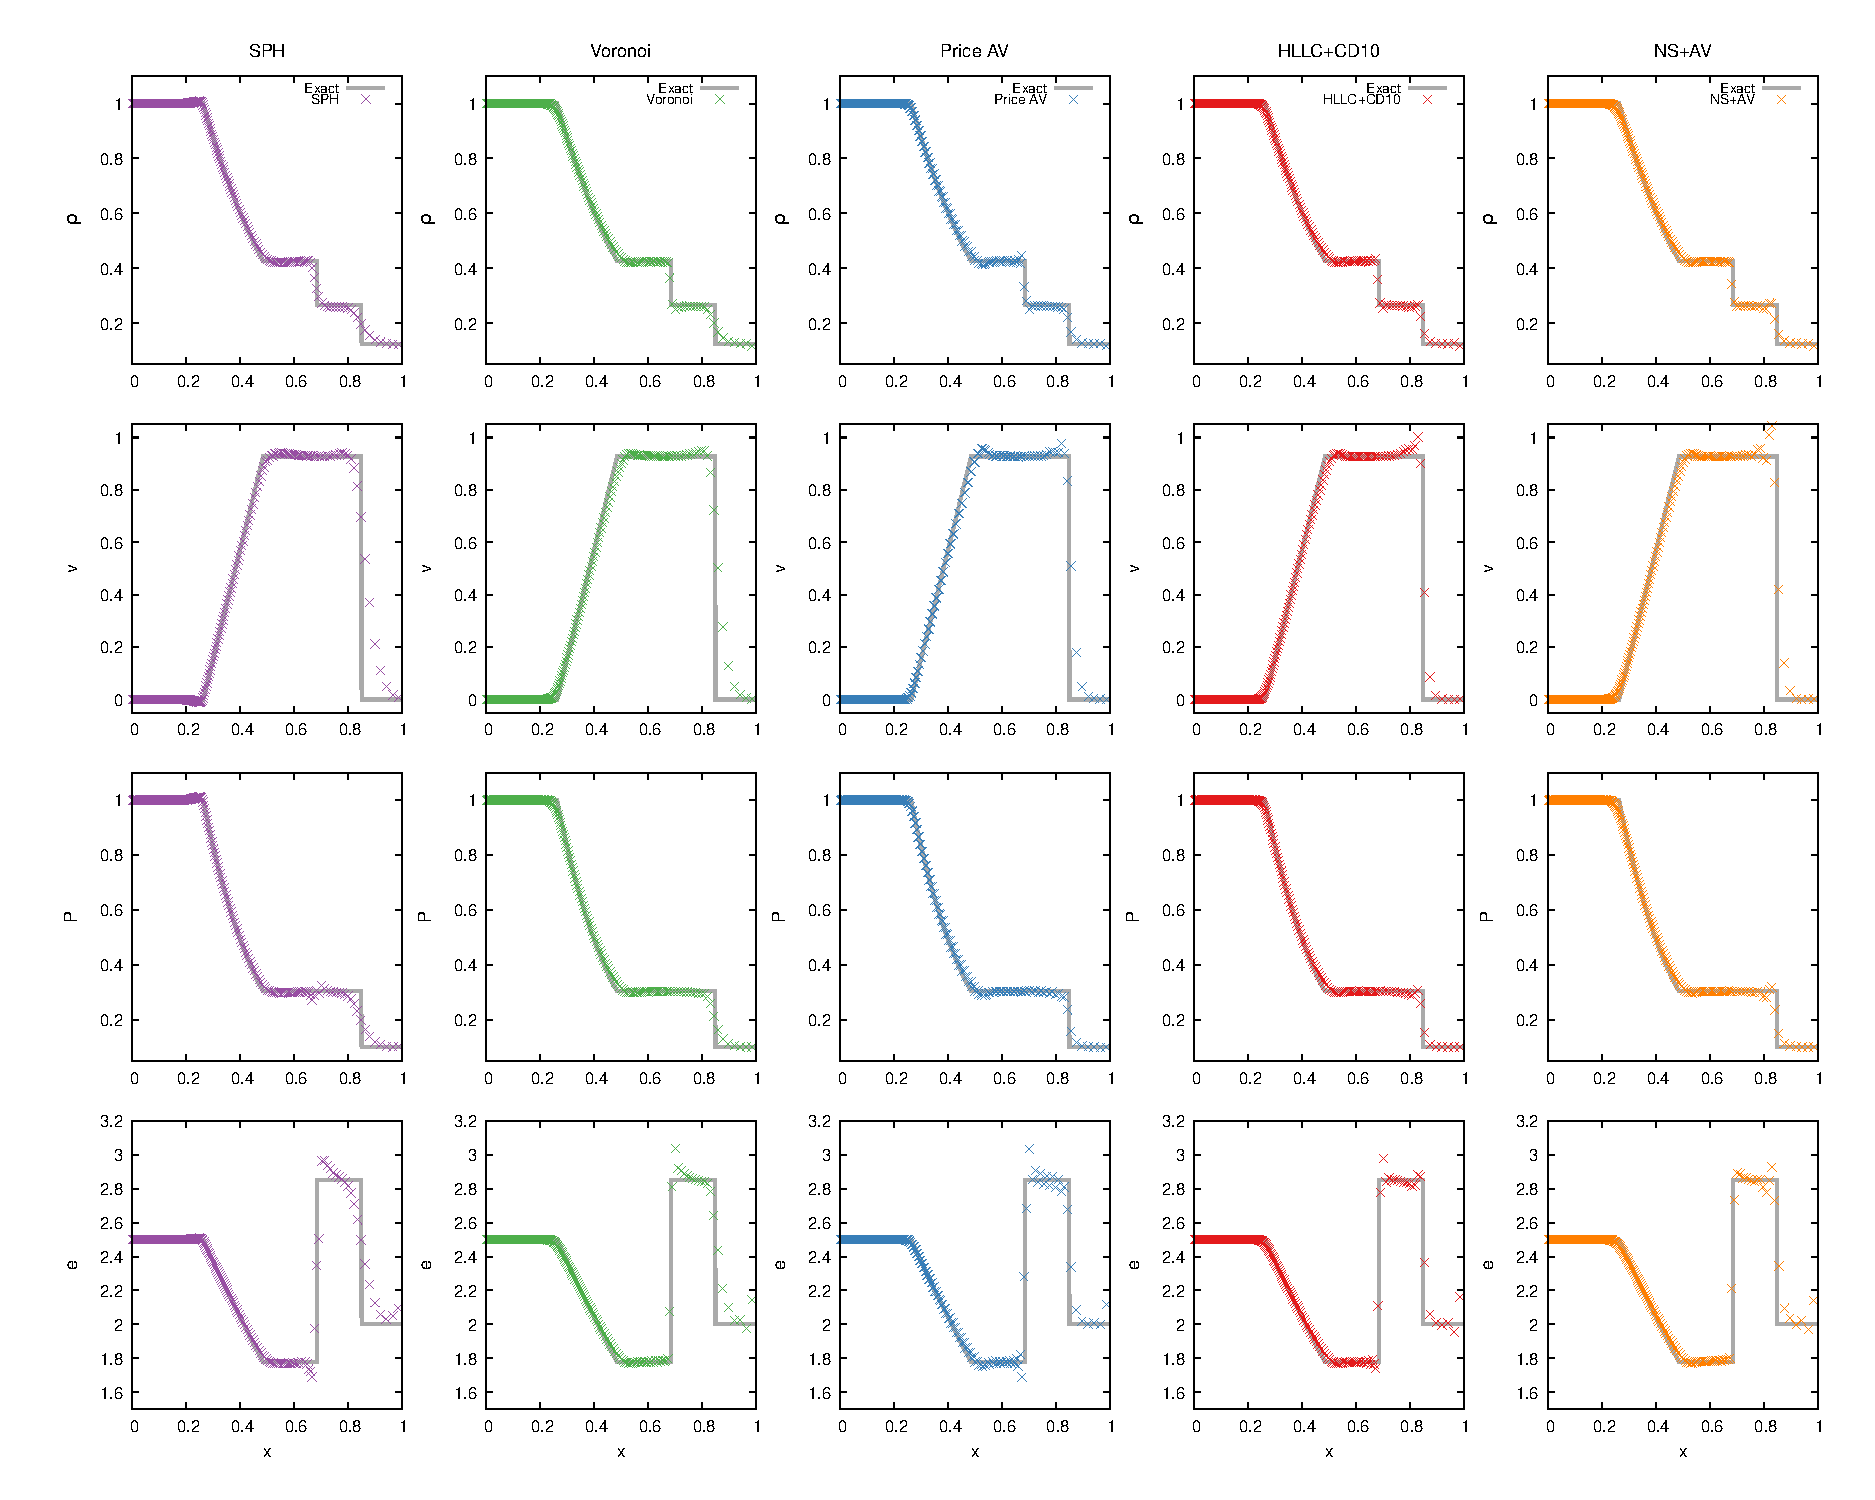
\includegraphics[width=\textwidth]{1d_sod.pdf}
\caption{Sod shock tube ($N=200$).
  Columns: SPH, Voronoi, Price~AV, HLLC+CD10, NS+AV.
  Rows: density, velocity, pressure, internal energy.
  Gray lines: exact solution;
  crosses: simulation results.}
\label{fig:sod}
\end{figure*}


\subsection{Interacting Blast Waves}

The Woodward--Colella interacting blast-wave problem
places two strong shocks in $0\le x\le 1$ with reflecting walls
and the initial pressure distribution
$(P_L,\, P_M,\, P_R) = (1000,\, 0.01,\, 100)$, $\rho=1$, and $\vel=0$.
The extreme pressure ratio ($\sim10^5$) makes this a severe test
for any Lagrangian method.
Figure~\ref{fig:blast} shows that
the Voronoi method best resolves the interacting shocks,
while SPH significantly smears the density peaks.
The HLLC+CD10 result overshoots the peak near $x\approx0.76$,
reflecting the sensitivity of the MUSCL reconstruction to the
extreme pressure gradient.
NS+AV ($L_1=8.87\times10^{-2}$) performs comparably to
HLLC+CD10 ($9.11\times10^{-2}$), capturing the density
peaks without the overshoot seen in the Riemann-solver approach.

\begin{figure*}[htbp!]
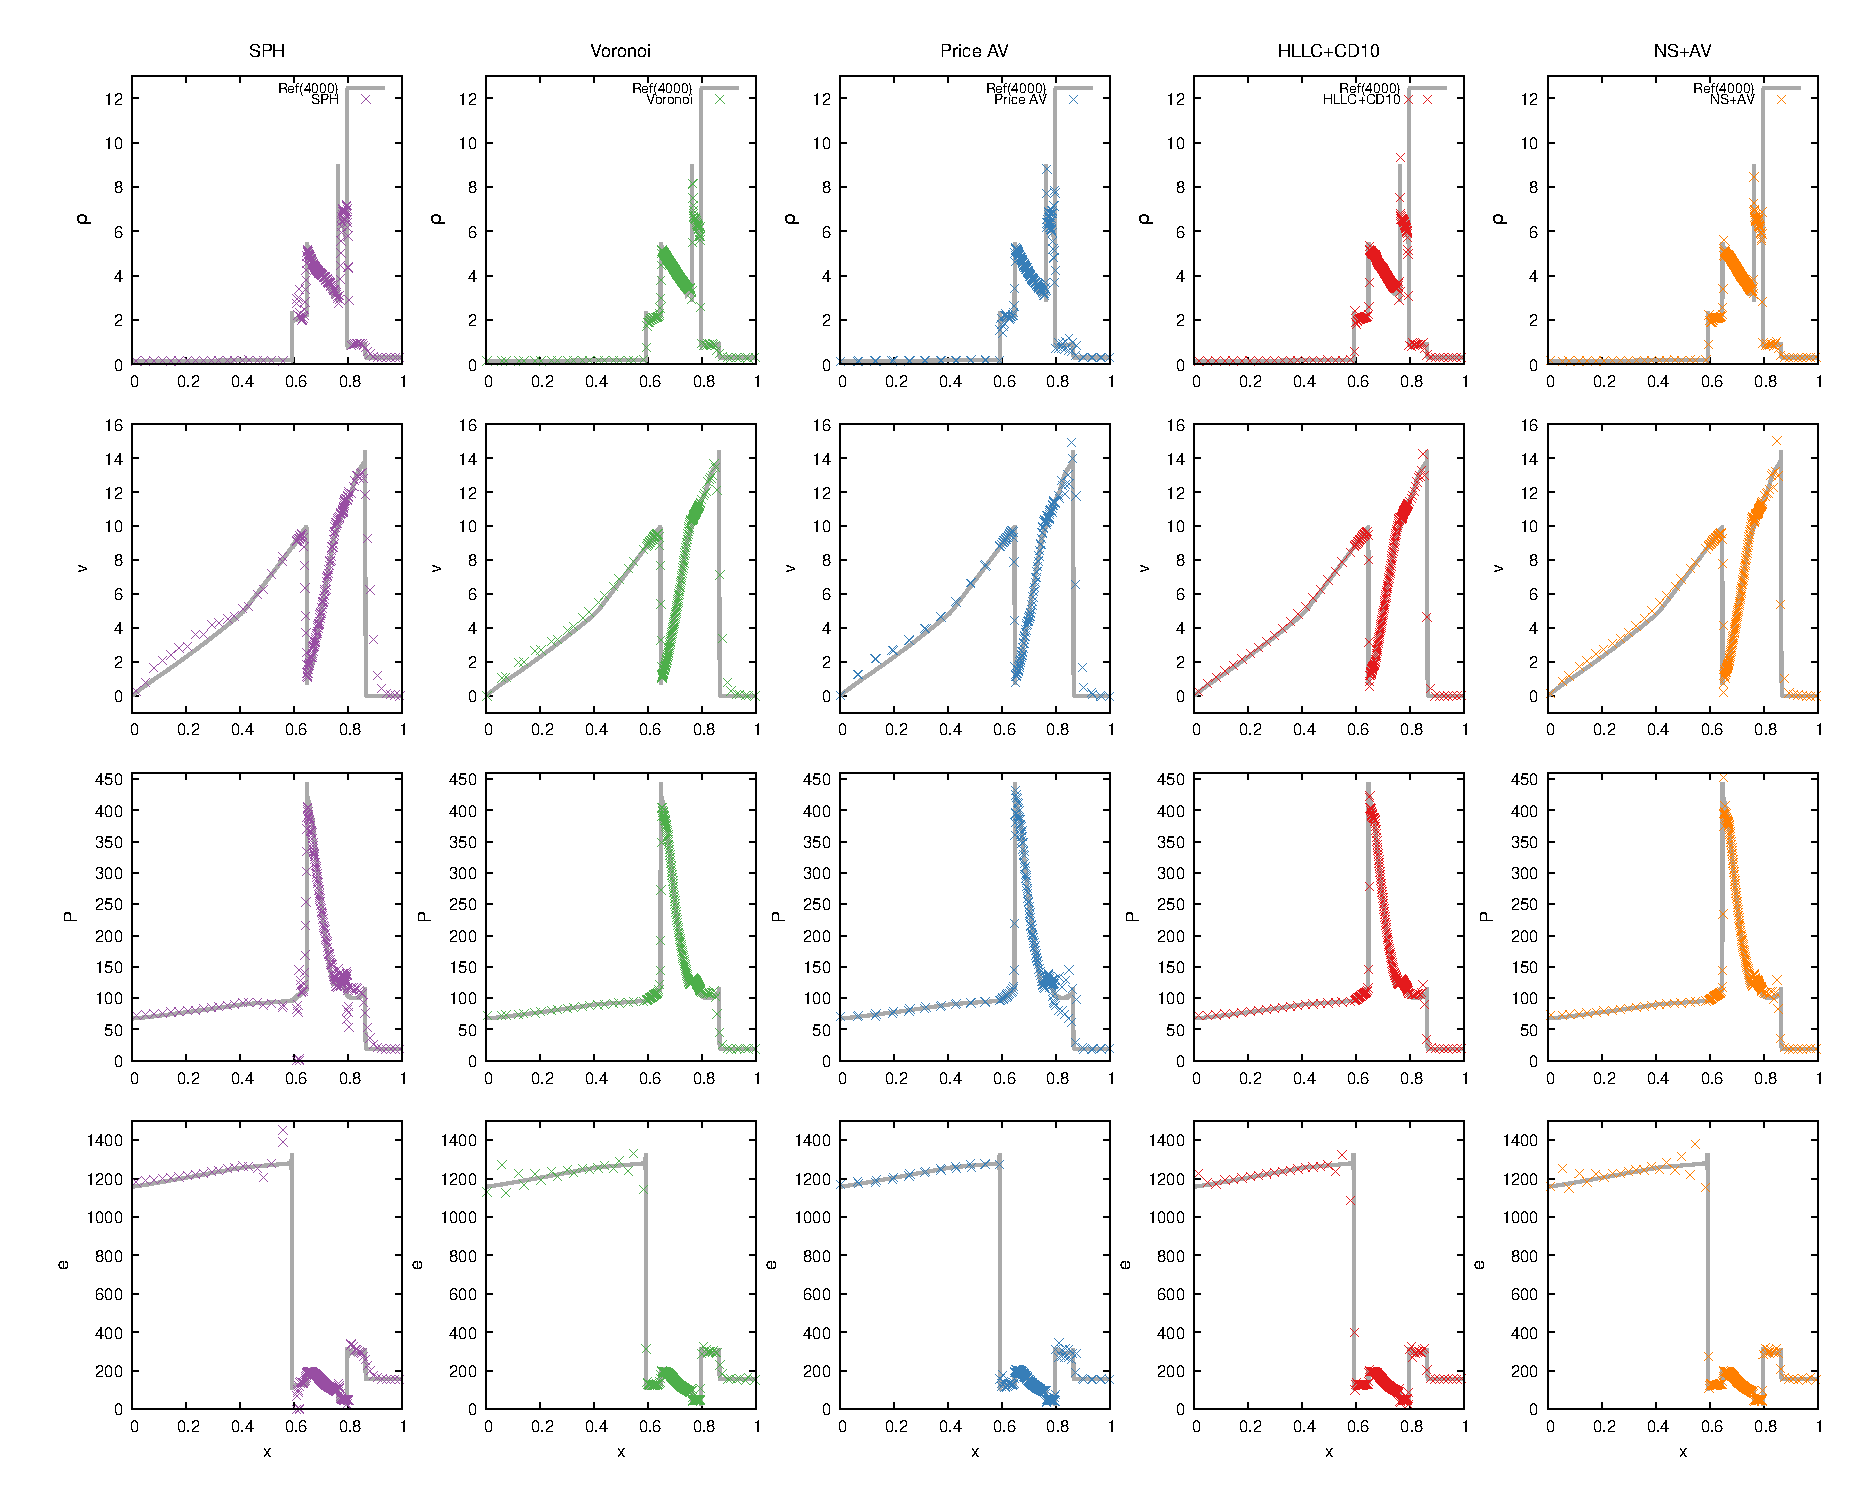
\includegraphics[width=\textwidth]{1d_blast.pdf}
\caption{Interacting blast waves ($N=200$).
  Columns: SPH, Voronoi, Price~AV, HLLC+CD10, NS+AV.
  Rows: density, velocity, pressure, internal energy.
  Gray lines: high-resolution reference ($N=4000$);
  crosses: simulation results.}
\label{fig:blast}
\end{figure*}


\subsection{Noh Strong Shock}

The Noh problem features a cold gas ($e=10^{-6}$) converging
at $\vel=-1$ toward a reflecting wall at $x=0$ with $\gamma=5/3$.
The exact solution is an outward-propagating strong shock at
$x_s = t/3$ behind which $\rho=4$ (the strong-shock compression
ratio for $\gamma=5/3$).
Figure~\ref{fig:noh} shows that all
Lagrangian methods except SPH achieve $L_1(\rho)\approx 0.02$,
accurately capturing the post-shock plateau at $\rho=4$
with only mild wall-heating at the reflecting boundary.
NS+AV achieves the best result ($L_1=2.05\times10^{-2}$),
slightly ahead of HLLC+CD10 ($2.18\times10^{-2}$).
SPH is notably worse ($L_1=1.08$) due to its kernel-smoothed
density estimate, which broadens the shock front.

\begin{figure*}[htbp!]
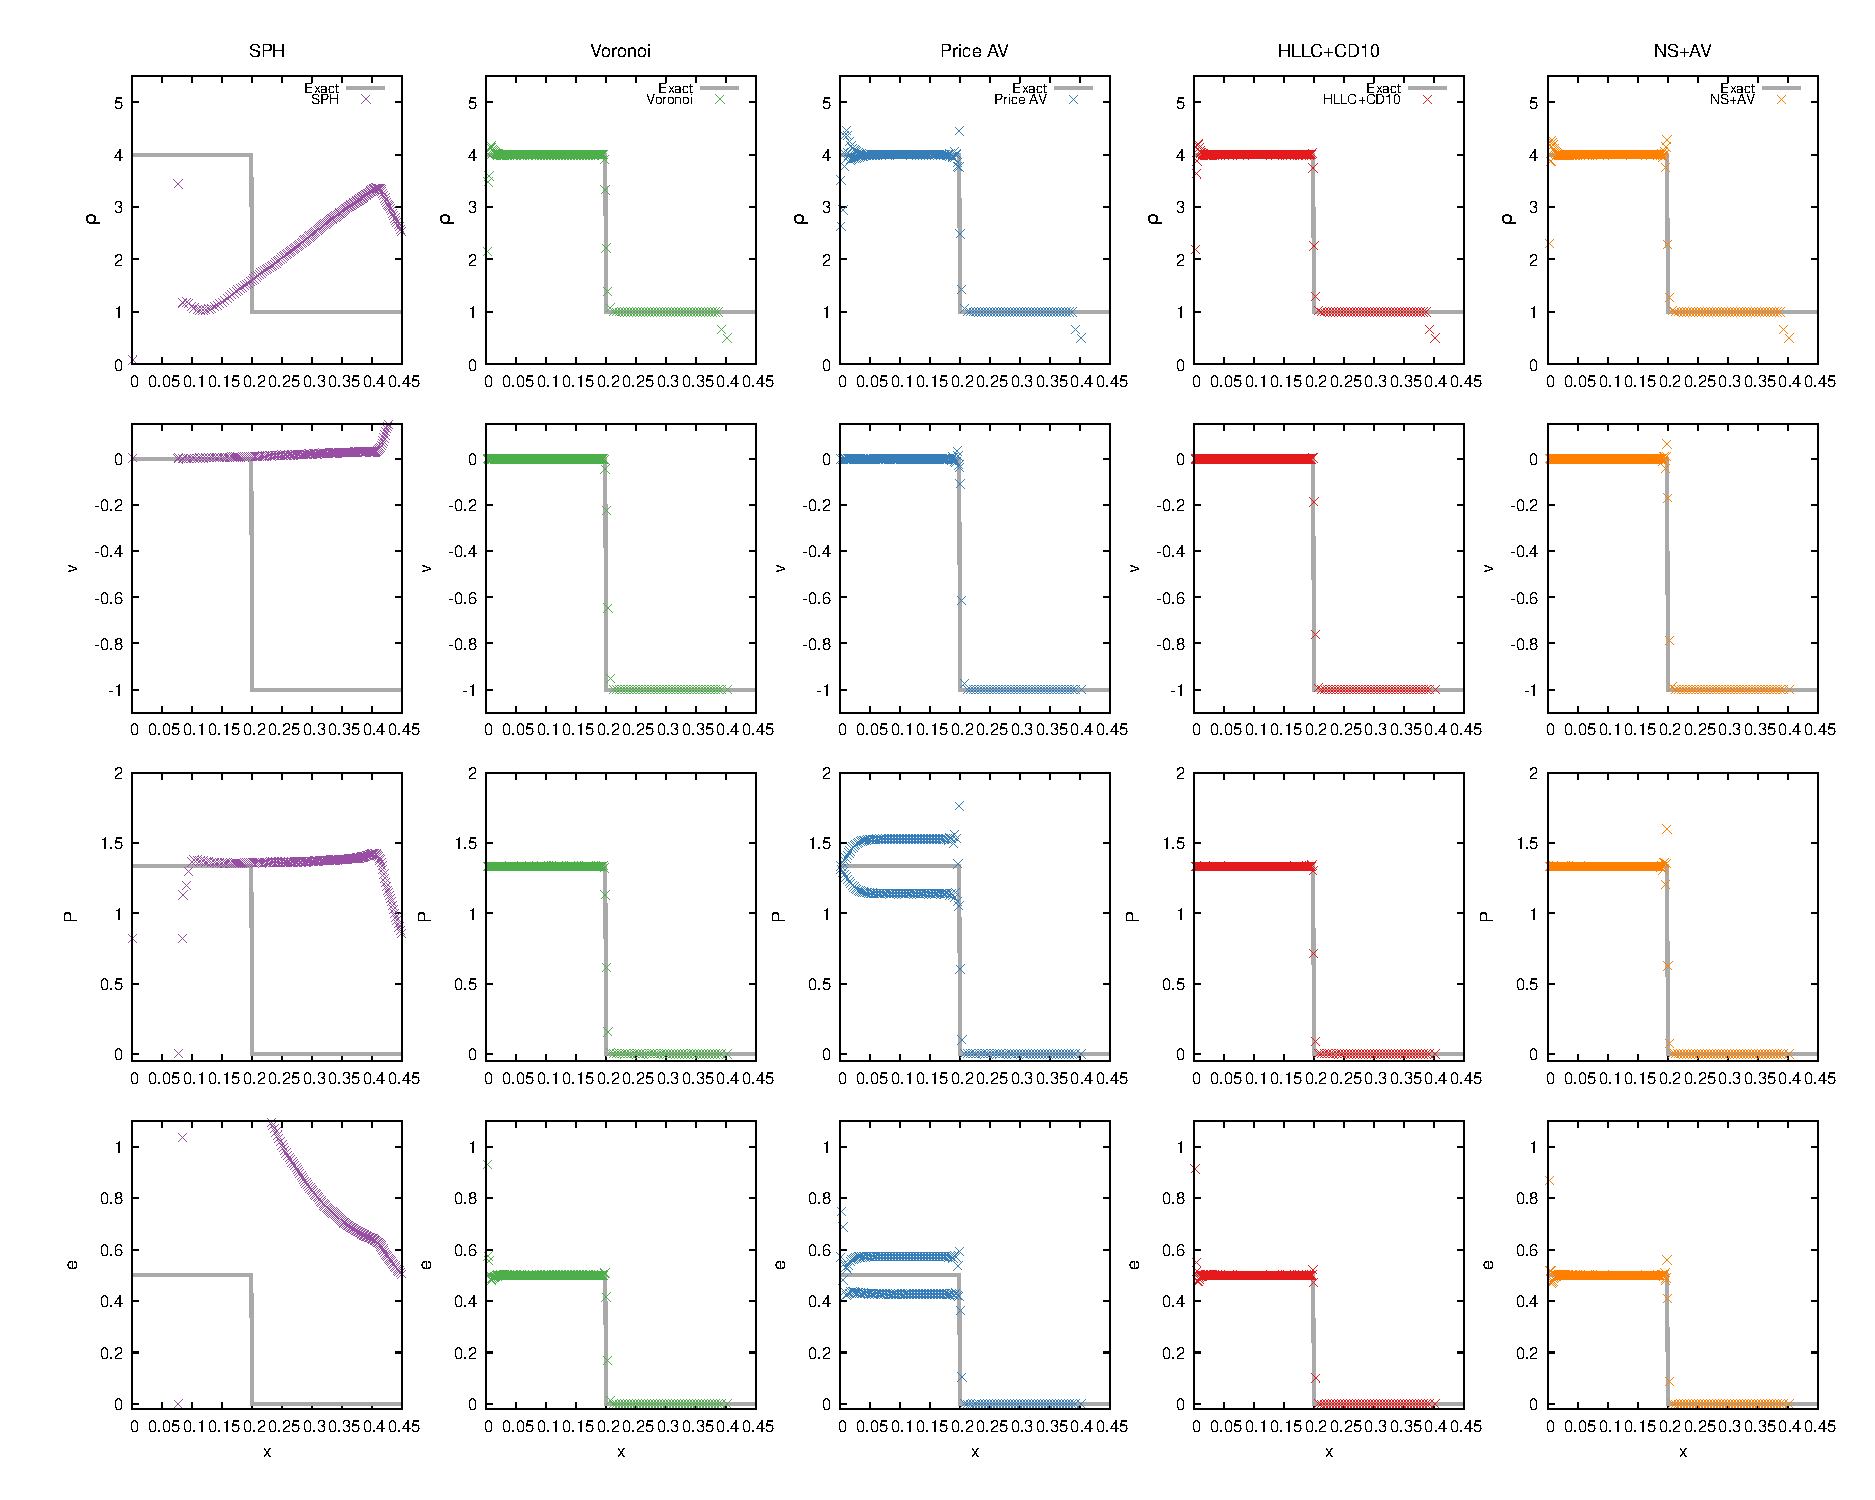
\includegraphics[width=\textwidth]{1d_noh.pdf}
\caption{Noh strong shock ($N=200$).
  Columns: SPH, Voronoi, Price~AV, HLLC+CD10, NS+AV.
  Rows: density, velocity, pressure, internal energy.
  Gray lines: exact solution;
  crosses: simulation results.}
\label{fig:noh}
\end{figure*}


\subsection{Shu--Osher Shock-Entropy Interaction}

The Shu--Osher problem propagates a Mach-3 shock into
a sinusoidally perturbed density field
($\rho = 1+0.2\sin 5x$ for $x>-4$) on $-5\le x\le5$
with transmissive boundaries.
The interaction generates high-frequency entropy waves
behind the shock, testing a method's ability to preserve
small-scale structure.
Figure~\ref{fig:shuosher} shows that
SPH severely damps the post-shock oscillations.
NS+AV best preserves the entropy waves
($L_1=6.00\times10^{-1}$), surpassing HLLC+CD10
($6.93\times10^{-1}$).
The NS viscous stress provides less dissipation
in smooth oscillatory regions than the Cullen--Dehnen switch,
allowing finer structure to survive.
Voronoi ($1.24$) and Price~AV ($2.74$) suffer from
excessive diffusion of the post-shock density peaks
at this resolution.
These transmissive runs do not insert post-shock gas, so the shock remains near $x\simeq 1.8$. The GFS result with inflow is Figure~\ref{fig:gfs1d}.

\begin{figure*}[htbp!]
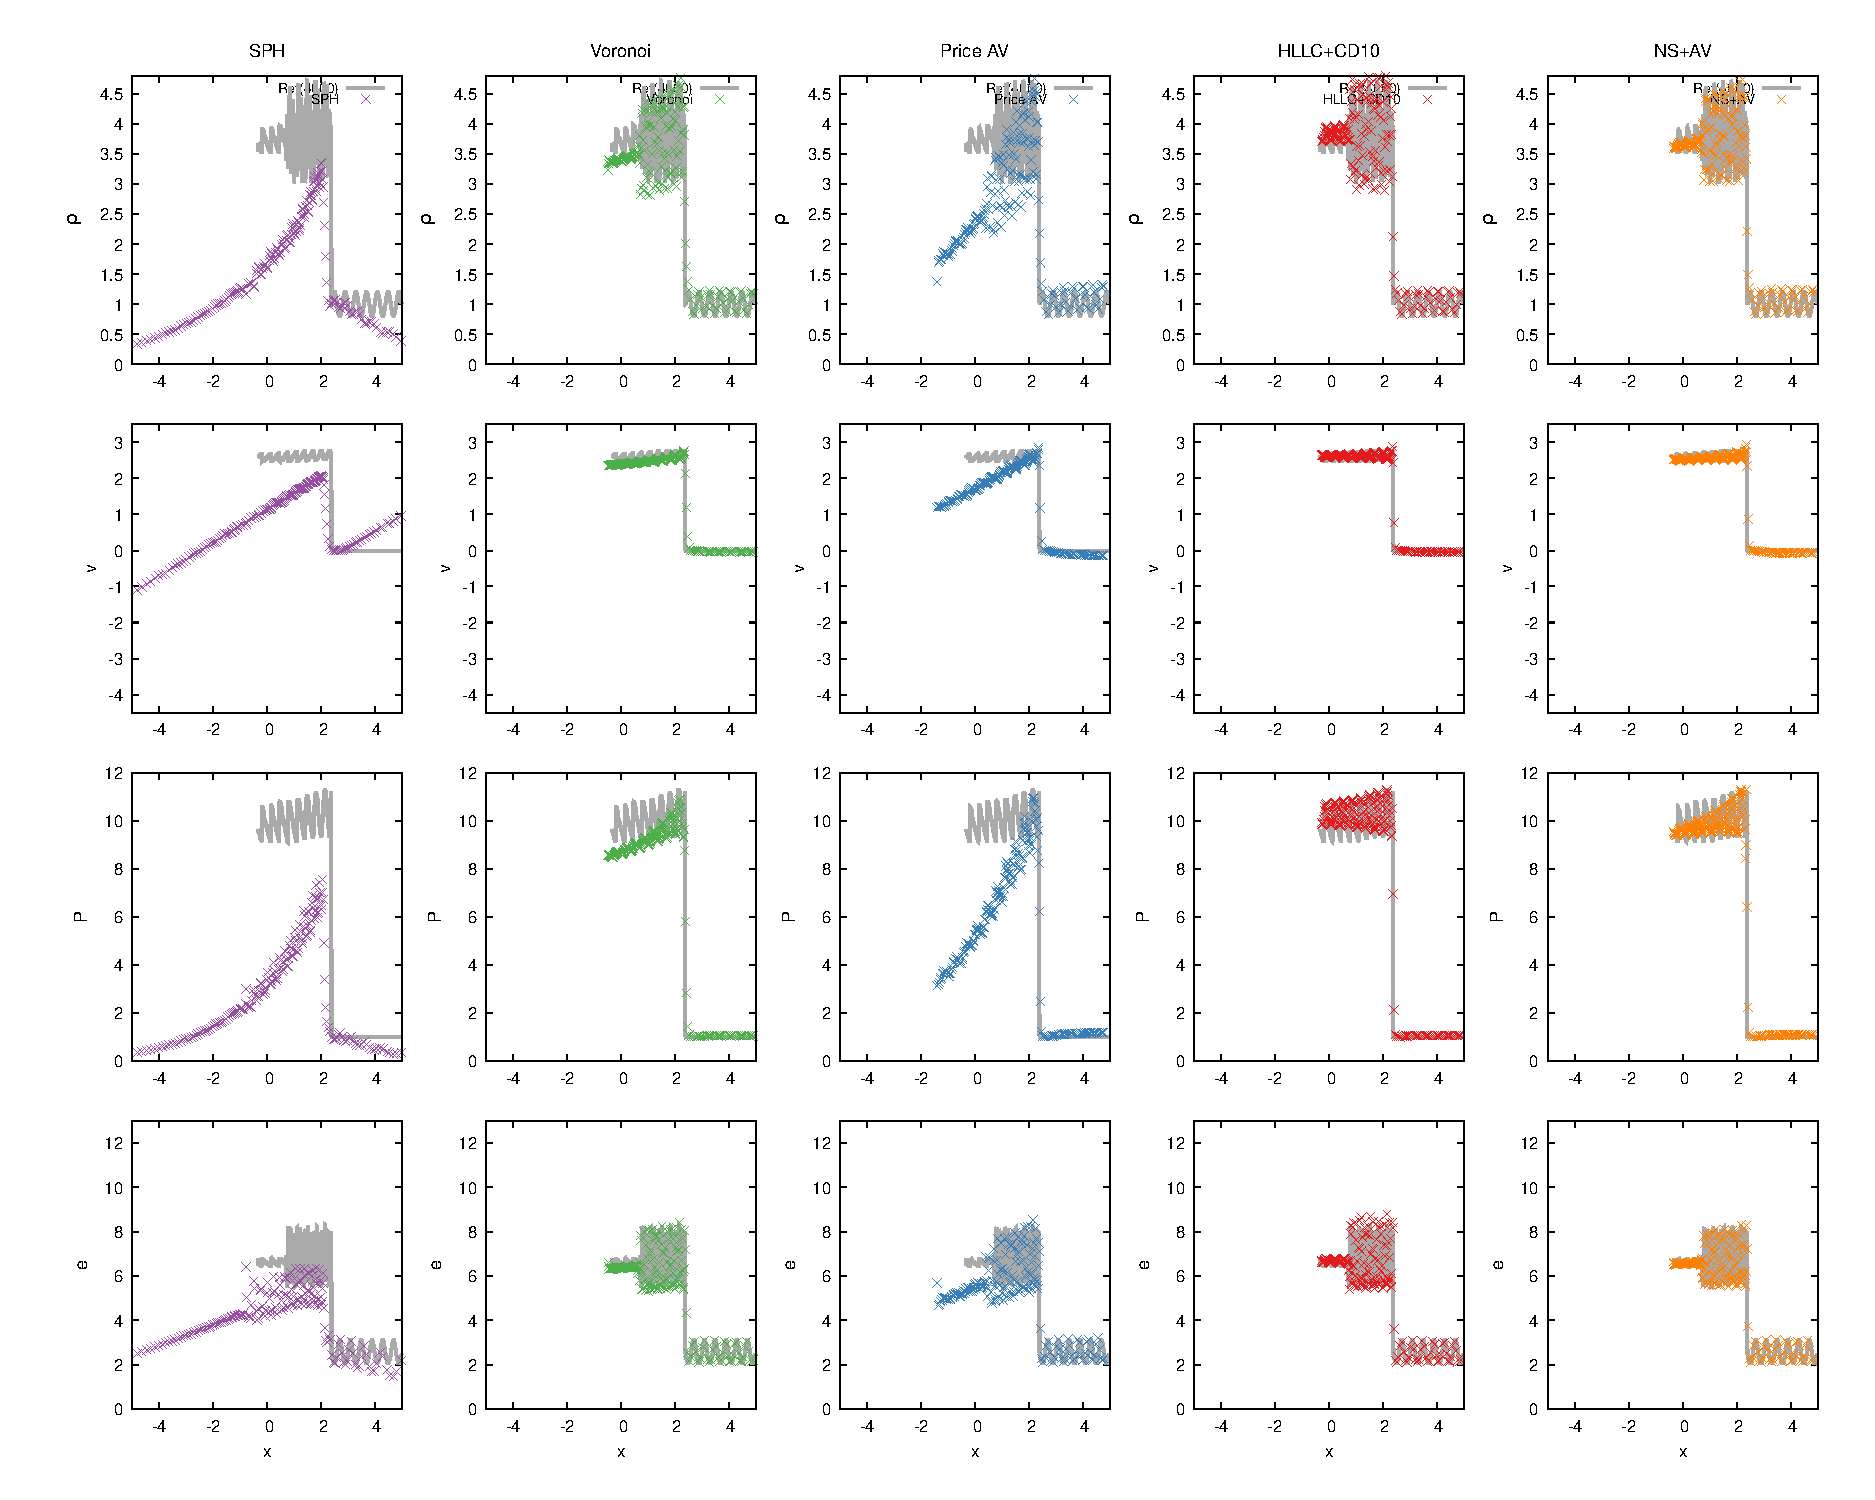
\includegraphics[width=\textwidth]{1d_shuosher.pdf}
\caption{Shu--Osher shock-entropy interaction ($N=200$).
  Columns: SPH, Voronoi, Price~AV, HLLC+CD10, NS+AV.
  Rows: density, velocity, pressure, internal energy.
  Gray lines: high-resolution reference ($N=4000$);
  crosses: simulation results.}
\label{fig:shuosher}
\end{figure*}



\subsection{Lax Shock Tube}

The Lax problem \citep{LaxWendroff1960} is a Riemann problem
with non-zero initial velocity on the left state:
$(\rho,P,\vel)_L=(0.445,\,3.528,\,0.698)$ and
$(\rho,P,\vel)_R=(0.5,\,0.571,\,0)$ for $x\ge0.5$,
with transmissive boundaries and $t_\mathrm{end}=0.13$.
This test produces a strong shock, a contact discontinuity,
and a rarefaction fan, similar to the Sod problem but with
a faster-moving contact wave.
Figure~\ref{fig:lax} shows that the four non-SPH Lagrangian methods
produce excellent results ($L_1\approx5\times10^{-3}$),
with NS+AV ($5.41\times10^{-3}$) competitive with the others.
SPH fails to resolve the contact discontinuity
($L_1=6.52\times10^{-1}$).

\begin{figure*}[htbp!]
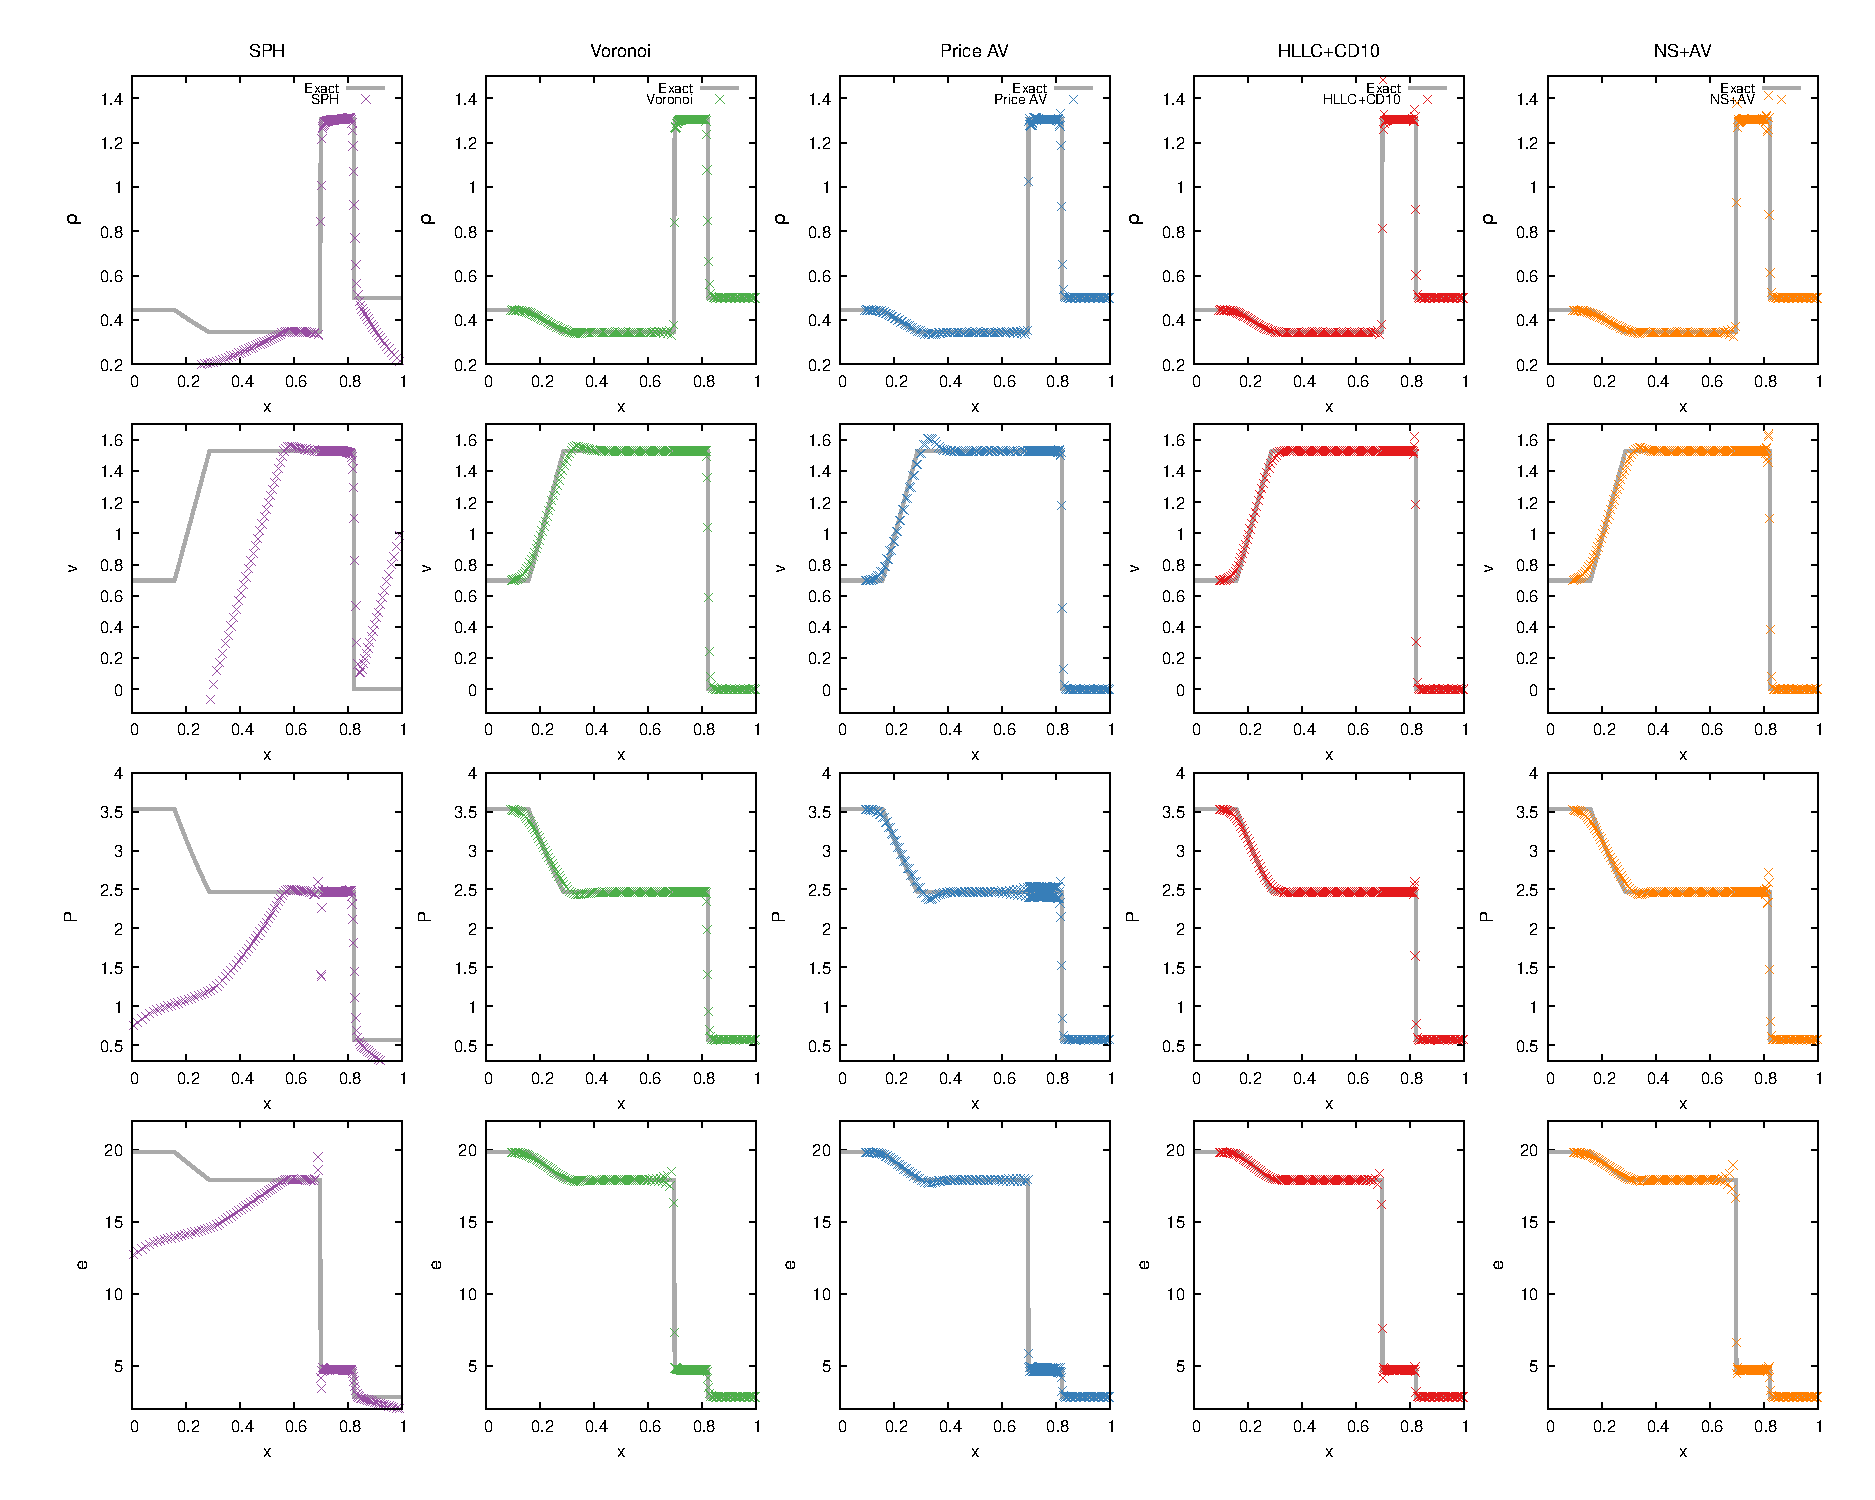
\includegraphics[width=\textwidth]{1d_lax.pdf}
\caption{Lax shock tube ($N=200$).
  Columns: SPH, Voronoi, Price~AV, HLLC+CD10, NS+AV.
  Rows: density, velocity, pressure, internal energy.
  Gray lines: exact solution;
  crosses: simulation results.}
\label{fig:lax}
\end{figure*}


\subsection{Double Rarefaction}

The double rarefaction (Toro test~\#2) initializes two
symmetric rarefaction waves diverging from $x=0.5$:
$(\rho,P,\vel)_L=(1,\,0.4,\,-2)$ and
$(\rho,P,\vel)_R=(1,\,0.4,\,+2)$, with transmissive
boundaries and $t_\mathrm{end}=0.15$.
This problem creates a near-vacuum region at the center
where the density drops to $\rho\approx0.02$ and the
pressure approaches zero.
Figure~\ref{fig:dblfan} shows that the Lagrangian methods
accurately resolve the double rarefaction structure,
with HLLC+CD10 achieving $L_1=2.56\times10^{-2}$,
followed by NS+AV ($3.32\times10^{-2}$) and
Voronoi and Price~AV at $L_1\approx3.8$--$3.9\times10^{-2}$.
SPH performs significantly worse ($L_1=5.08\times10^{-1}$)
due to difficulty resolving the near-vacuum region.

\begin{figure*}[htbp!]
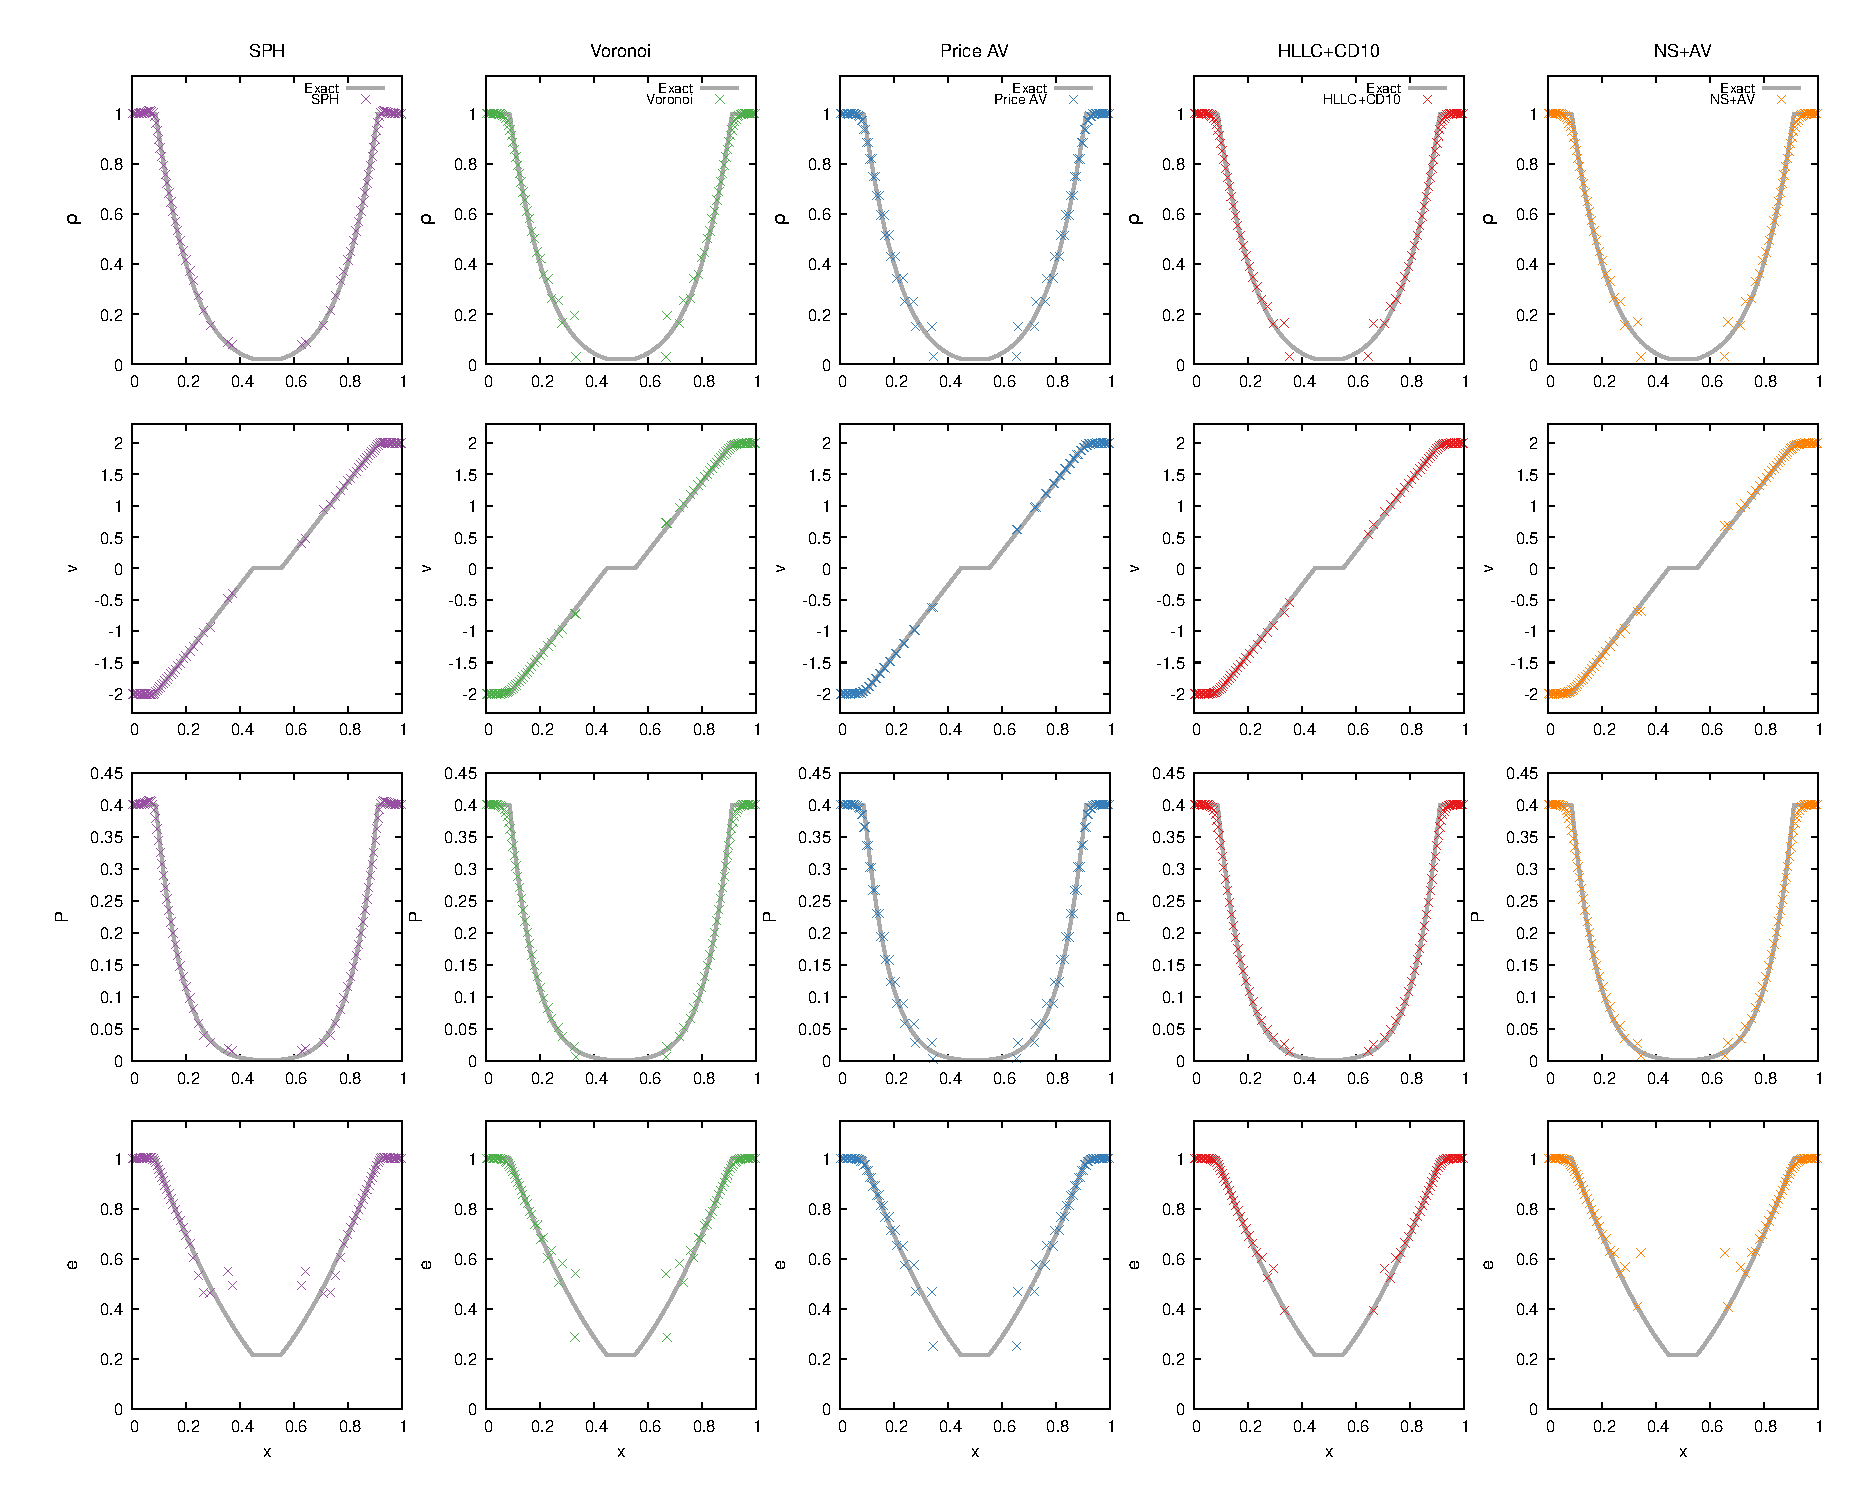
\includegraphics[width=\textwidth]{1d_dblfan.pdf}
\caption{Double rarefaction ($N=200$).
  Columns: SPH, Voronoi, Price~AV, HLLC+CD10, NS+AV.
  Rows: density, velocity, pressure, internal energy.
  Gray lines: exact solution;
  crosses: simulation results.}
\label{fig:dblfan}
\end{figure*}


\subsection{Two-Shock Collision}

The two-shock collision (Toro test~\#4) produces two
strong shocks colliding near $x=0.4$:
$(\rho,P,\vel)_L=(5.99924,\,460.894,\,19.5975)$ and
$(\rho,P,\vel)_R=(5.99242,\,46.095,\,-6.19633)$,
with transmissive boundaries and $t_\mathrm{end}=0.035$.
The solution contains two shocks, a contact discontinuity,
and a very high density peak ($\rho\approx31$).
Figure~\ref{fig:collision} shows that HLLC+CD10 best resolves
the density peak ($L_1=2.14\times10^{-1}$), with NS+AV
close behind ($2.44\times10^{-1}$) and Voronoi at
$3.70\times10^{-1}$.
Price~AV shows larger errors ($L_1=2.37$) from excessive
post-shock oscillations, and SPH performs worst ($L_1=7.20$).
Both boundaries are inflows. Insertion of the exterior state at $N=200$ reduces the density $L_1$ from $0.47$ to $0.078$. The energy error of that calculation is $1.6\times10^{-5}$.

\begin{figure*}[htbp!]
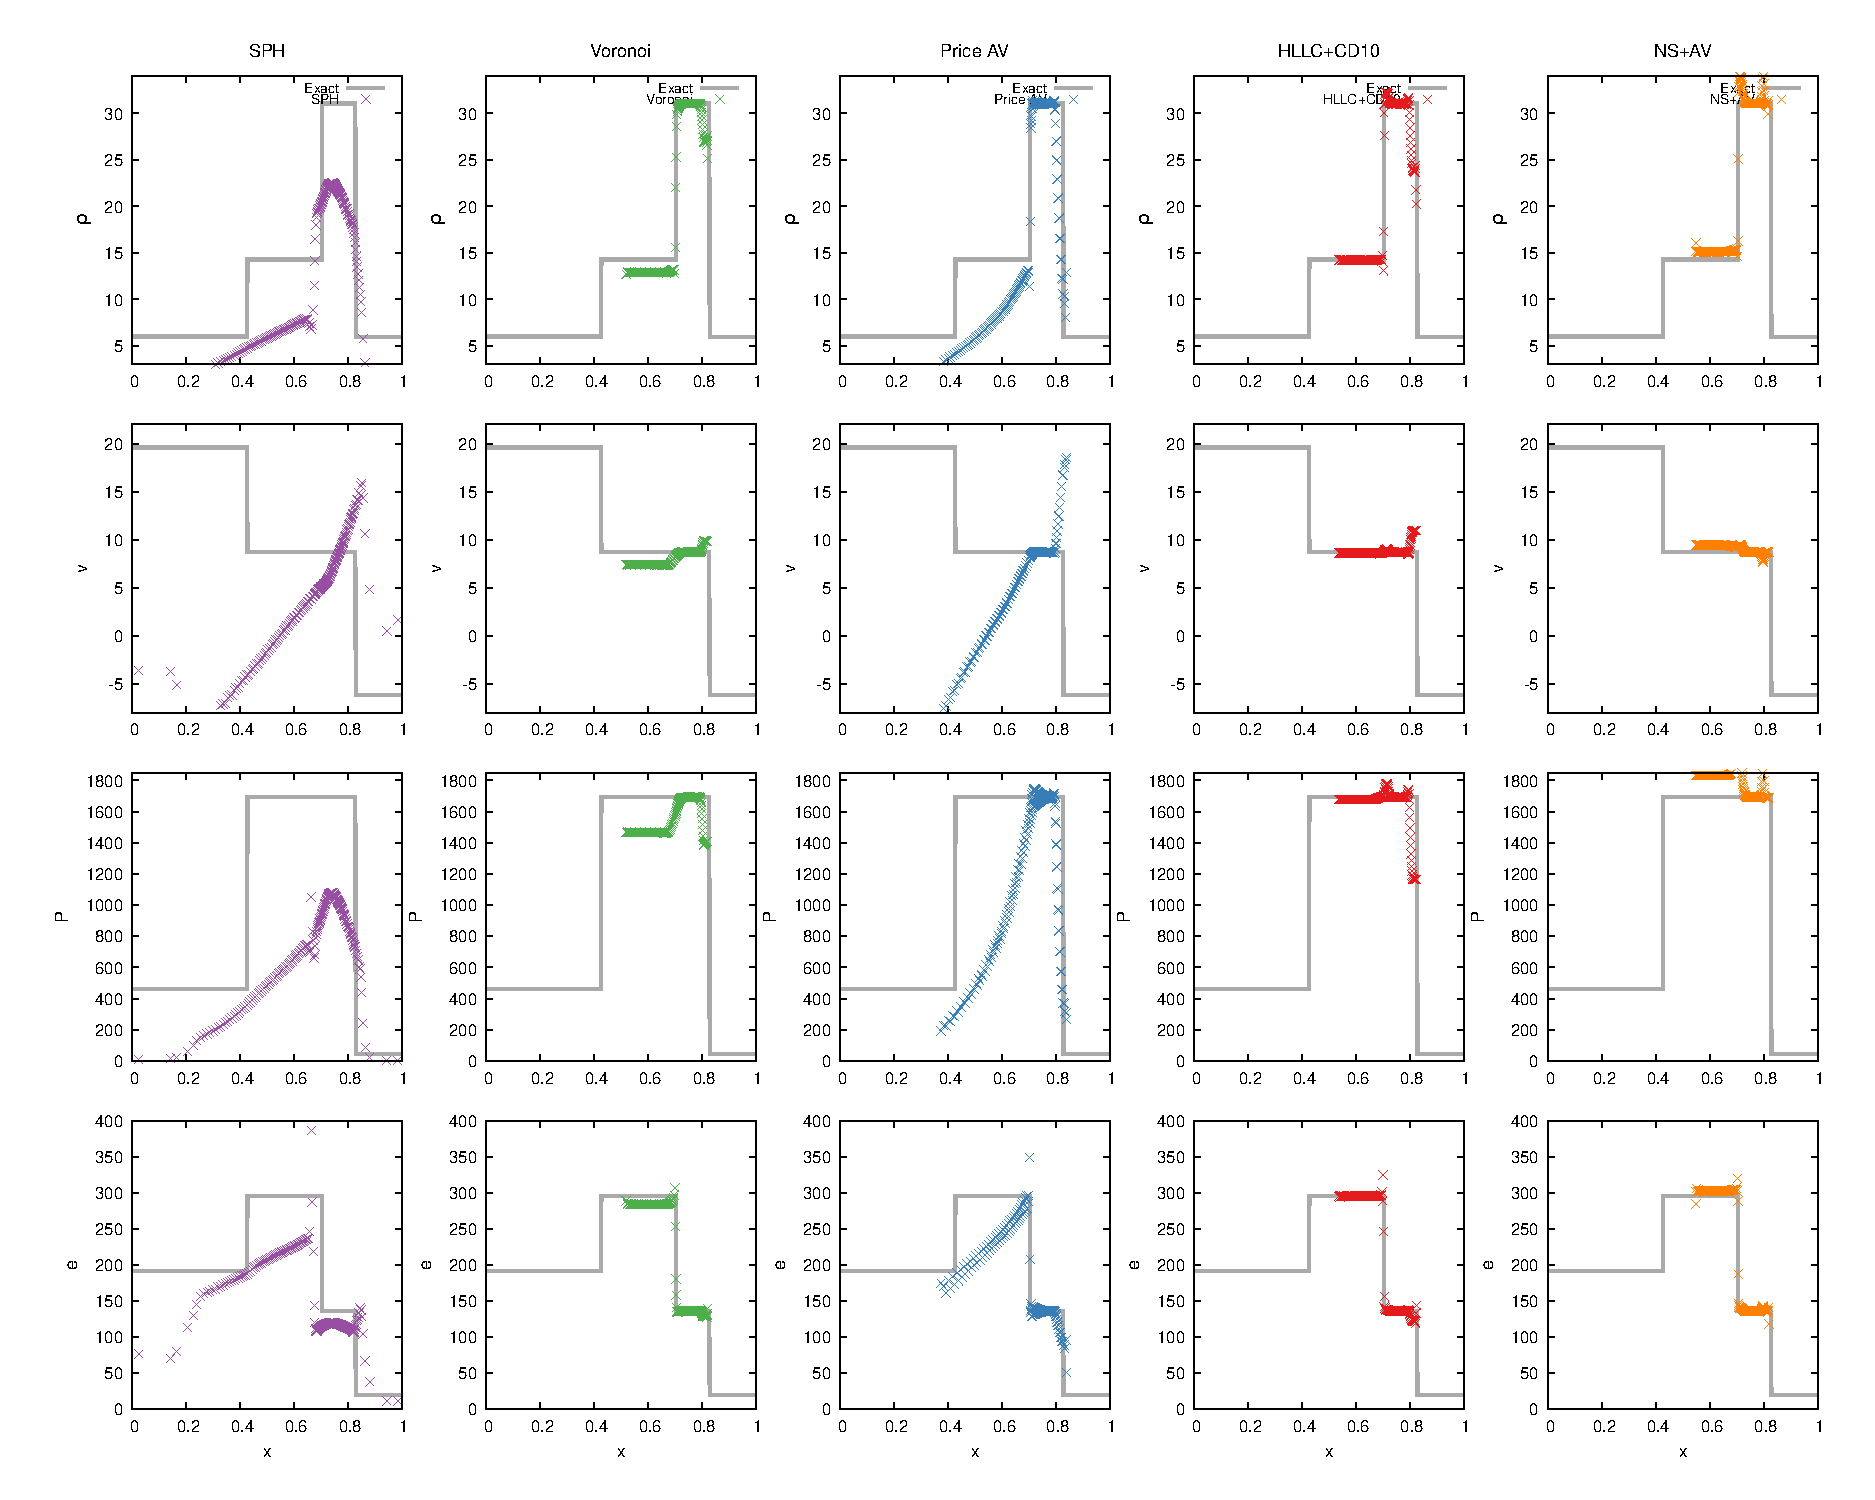
\includegraphics[width=\textwidth]{1d_collision.pdf}
\caption{Two-shock collision ($N=200$).
  Columns: SPH, Voronoi, Price~AV, HLLC+CD10, NS+AV.
  Rows: density, velocity, pressure, internal energy.
  Gray lines: exact solution;
  crosses: simulation results.}
\label{fig:collision}
\end{figure*}


\subsection{Stationary Contact Discontinuity}

The stationary contact test isolates the contact
discontinuity by imposing equal pressures on both
sides:
$(\rho,P,\vel)_L=(1,\,1,\,0)$ and
$(\rho,P,\vel)_R=(0.125,\,1,\,0)$ for $x\ge0.5$,
with transmissive boundaries and $t_\mathrm{end}=0.25$.
The exact solution is a stationary density jump at $x=0.5$
with zero velocity and uniform pressure everywhere.
Figure~\ref{fig:contact} shows that the NS+AV method
achieves the sharpest contact resolution
($L_1=4.67\times10^{-3}$), closely followed by
Voronoi ($5.23\times10^{-3}$),
HLLC+CD10 ($5.71\times10^{-3}$), and Price~AV ($7.30\times10^{-3}$).
The NS viscous stress, being proportional to $\partial v/\partial x$,
vanishes identically at a stationary contact where $v=0$
everywhere, providing no spurious diffusion of the density jump.
SPH completely smears the contact ($L_1=1.03$),
illustrating the well-known zeroth-order inconsistency
of the kernel density estimate at sharp discontinuities.

\begin{figure*}[htbp!]
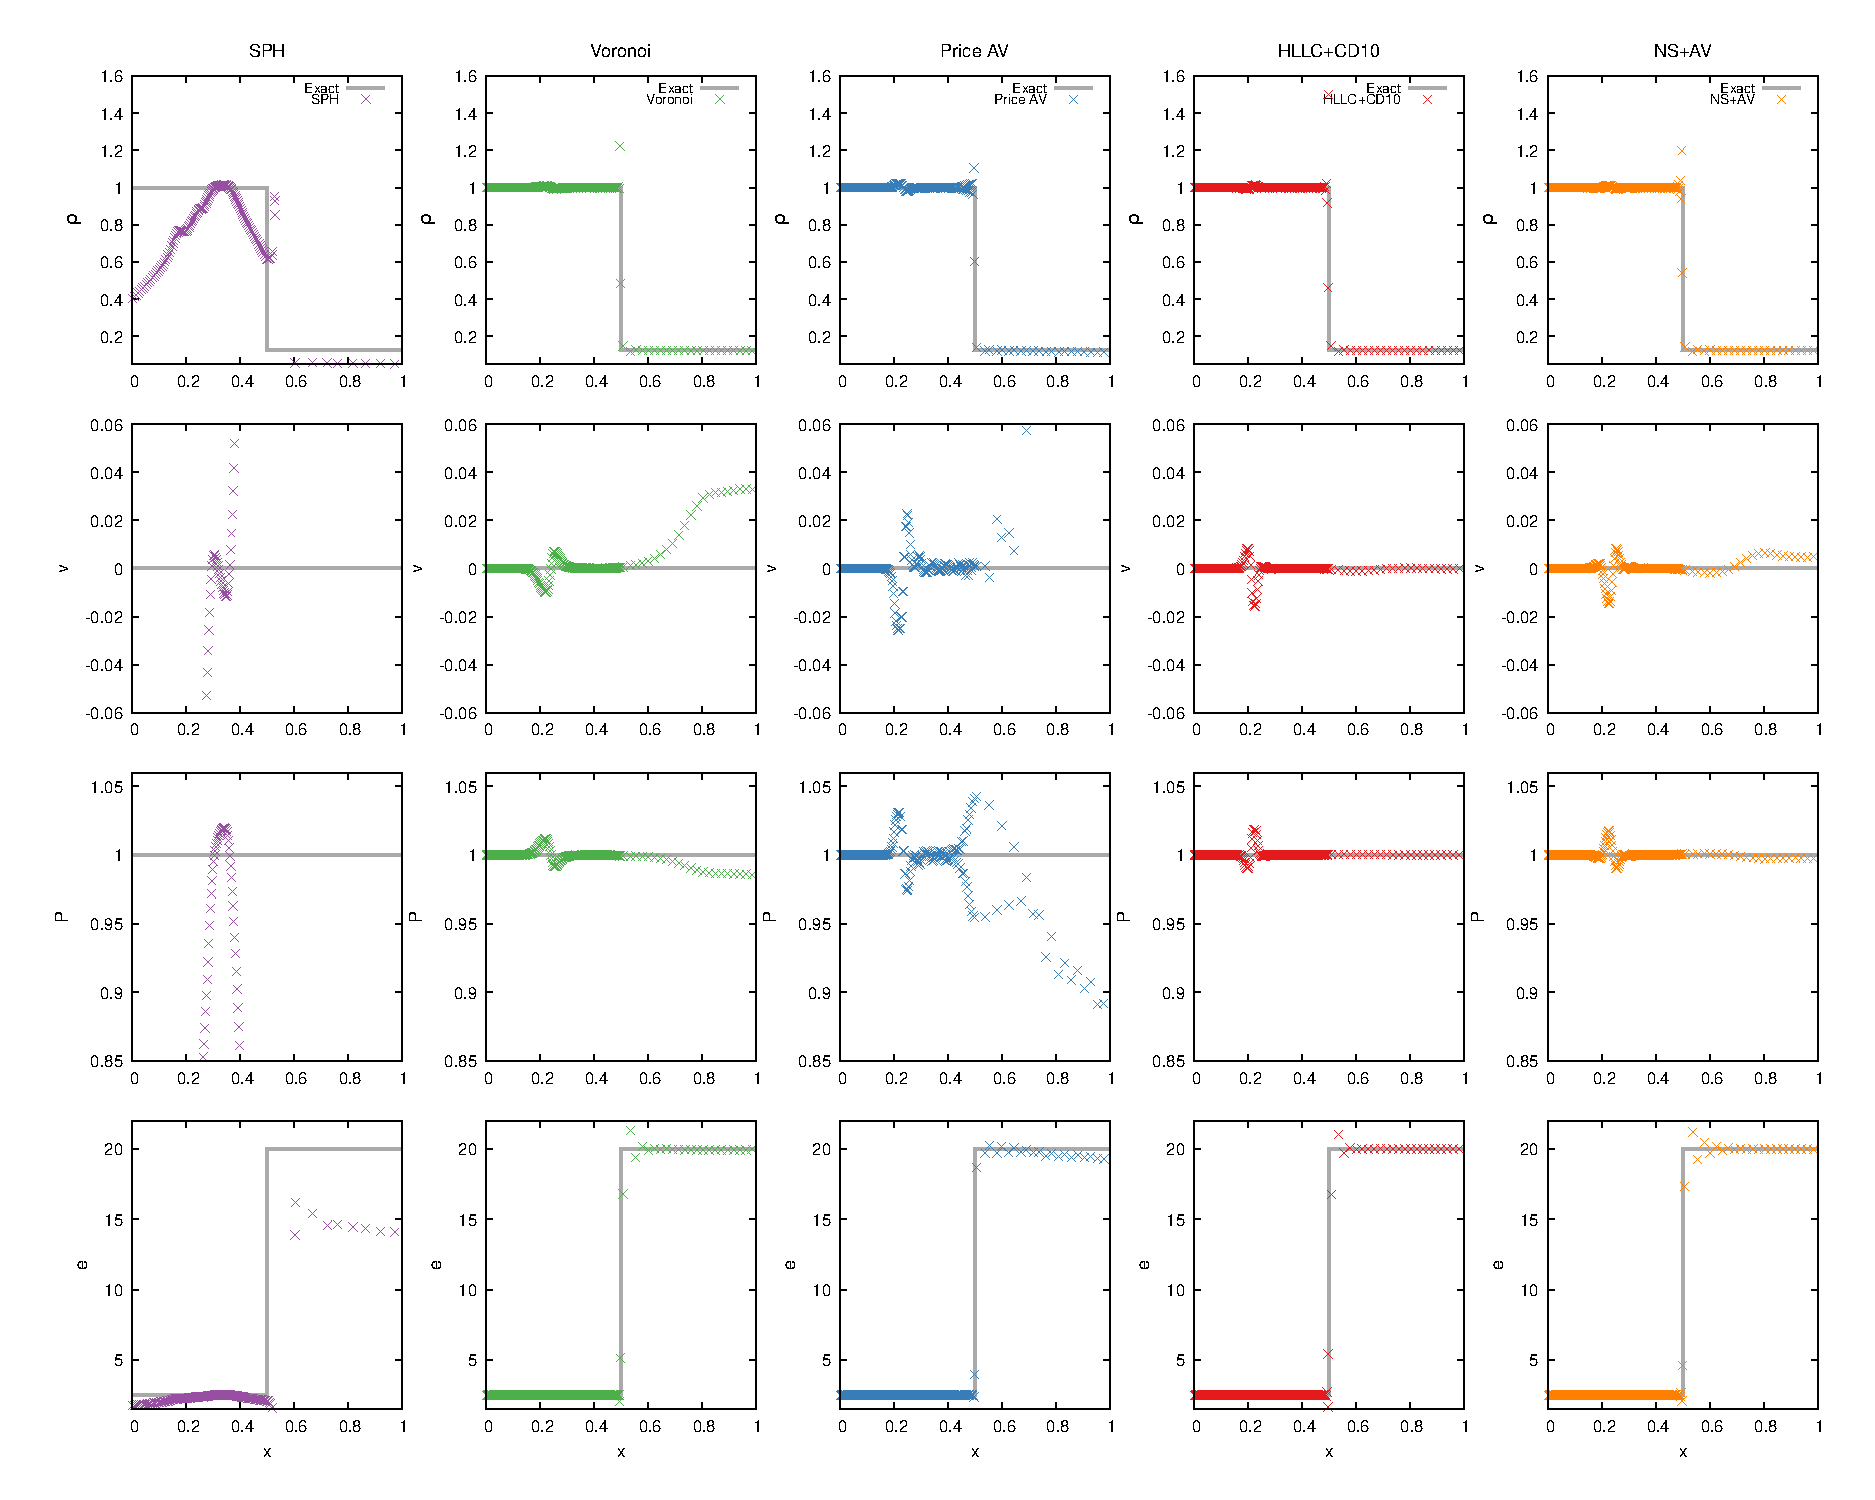
\includegraphics[width=\textwidth]{1d_contact.pdf}
\caption{Stationary contact discontinuity ($N=200$).
  Columns: SPH, Voronoi, Price~AV, HLLC+CD10, NS+AV.
  Rows: density, velocity, pressure, internal energy.
  Gray lines: exact solution;
  crosses: simulation results.}
\label{fig:contact}
\end{figure*}


\section{Conservation of Energy}
The energy conservation can be obtained by multiplying equation (\ref{basic1}) with the flow velocity, $\vel$, as 
\begin{eqnarray}
	 \vel\cdot\boldsymbol{f}_\text{ext} &=& \vel\cdot{\partial \over \partial t}(\rho\vel) + \vel\cdot\left\{\nabla\cdot(\rho\vel\vel)\right\} \\ \nonumber
	&=&  {\partial\over \partial t}(\rho \vel\cdot\vel) + \nabla\cdot\left\{\rho \vel (\vel\cdot\vel)\right\} - \rho\vel\cdot \left[
	{\partial\vel\over\partial t}-(\vel\cdot\nabla)\cdot\vel \right] \\
	&=& {\partial\over \partial t}(\rho \vel\cdot\vel) + \nabla\cdot\left\{\rho \vel (\vel\cdot\vel)\right\} -\vel\cdot\boldsymbol{f}_\text{ext},
\end{eqnarray}
which leads to
\begin{equation}
	{\partial \over \partial t}(\rho k) + \nabla\cdot(\rho k \vel) = \vel\cdot\boldsymbol{f}_\text{ext}
\end{equation}
where the kinetic energy of the flow is defined as $k \equiv (\vel\cdot\vel)/2$.


\section{Barycenter Interpolation} \label{baryinter}
In this section, we briefly describe the interpolation of polytrope in $N$ dimensional space.
Consider that there is $n$-sided polygon and assume the vertex of the polygon to be nodes to interpolate. Then, any point inside the polygon can be written by the affine combination of the nodes ($v_1, v_2, \cdots, v_n$) as
\begin{equation}
v = 	{\lambda_1 v_1 + \lambda_2 v_2\cdots +\lambda_n v_n \over \lambda_1 + \lambda_2 +\cdots + \lambda_n} = w_1v_1+w_2v_2+\cdots +w_nv_n
\end{equation} 
where $w_i \equiv \lambda_i/\Sigma_j \lambda_j$.

\begin{equation}
	\sum_{i=1}^n \lambda_i(v) (v_i-v) = 0
\end{equation}


%%%
\section{The Recursive Bisection To Generate Laguerre Diagram } \label{rbl}

For a given set of sites (or particles), we may generate the Laguerre cells. A Laguerre cell is defined as a set of positions which is closer to the site than any other site.
We employ a recursive bisection method (RBM) to construct the Voronoi cell of a given site. This spatial partitioning technique determines the volume where all interior positions are closest to the target site. The method can be summarized as follows: we first sort neighboring sites by their distance to the target site. Next, we place a large initial cube centered on the target. From the nearest neighboring site, we draw a bisectional plane (or line in 2D) between the neighbor and the target site, cutting away the outer volume. This process is iterated until the maximum distance of Voronoi-cell vertices from the center is less than twice the next neighboring distance, indicating that further bisection is no longer meaningful in constructing Voronoi cells.




Figure \ref{voro3d} illustrates how the BPM is working in the three dimensions. We initially set a big cubic Voronoi cell centered on the target site (top-left panel) and prune the  outer parts starting from the nearest neighbors. 
\begin{figure}[t!] 
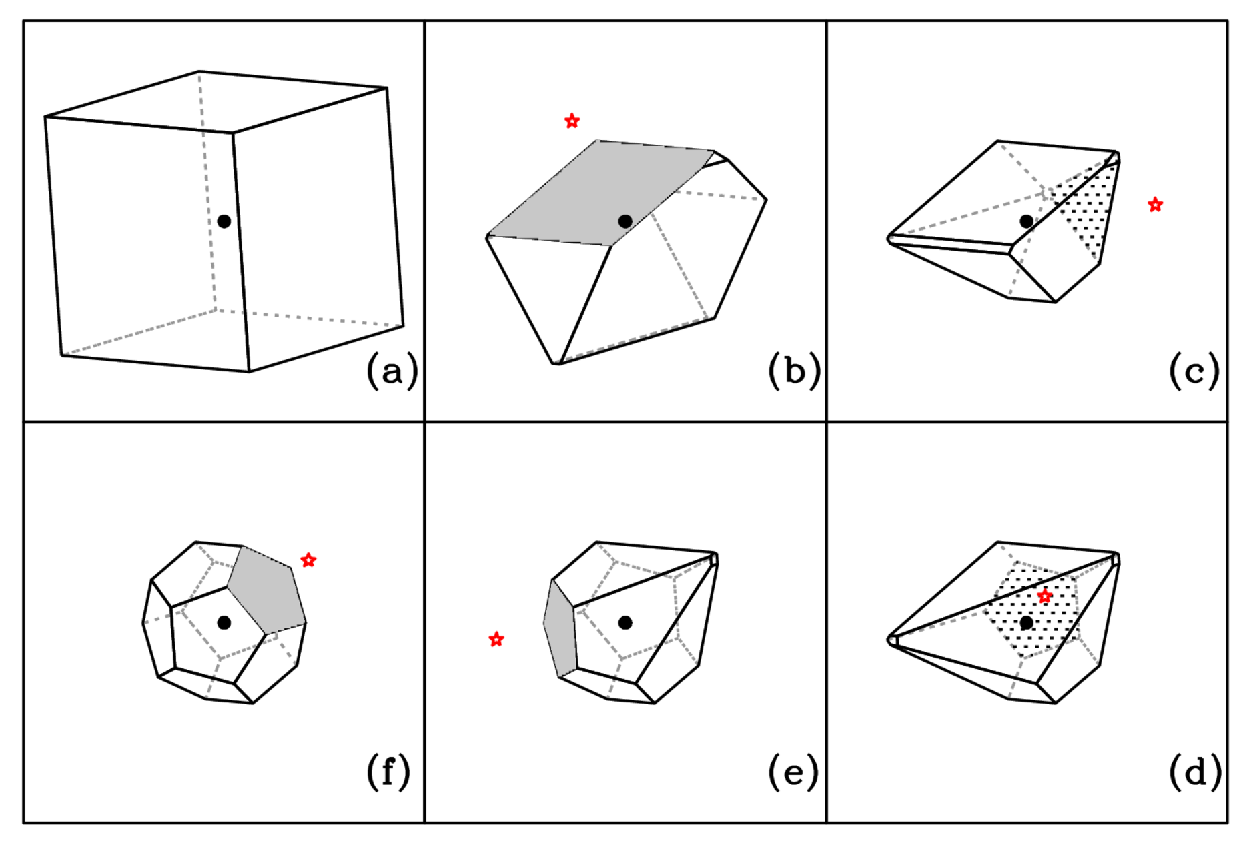
\includegraphics[width=\columnwidth]{cut3d.pdf}	
\caption{Illustration of the three-dimensional Voronoi cell construction  using the BPM. Clockwise from the top left panel we show the update of the Voronoi cell with applying neighbors (red star symbols) one by one. The black circle is the target site. In this figure, we show only a few pruning snapshots (initial shape, 5'th, 8'th, 10'th, 11'th, and 12'th neighbors). To shape this regular dodecahedron we use twelve vertices of the regular icosahedron as neighboring points in the BPM}
\label{voro3d}
\end{figure}

 An example of generating the 2D Laguerre cells is shown in Figure \ref{voro2d}. The black dots are the semi-randomly distributed particles and their corresponding Laguerre cells are painted in various colors. Here, the semi-random means that we place particle at the regular grid points and randomly perturb their positions within the grid cells.
\begin{figure}[t!] 
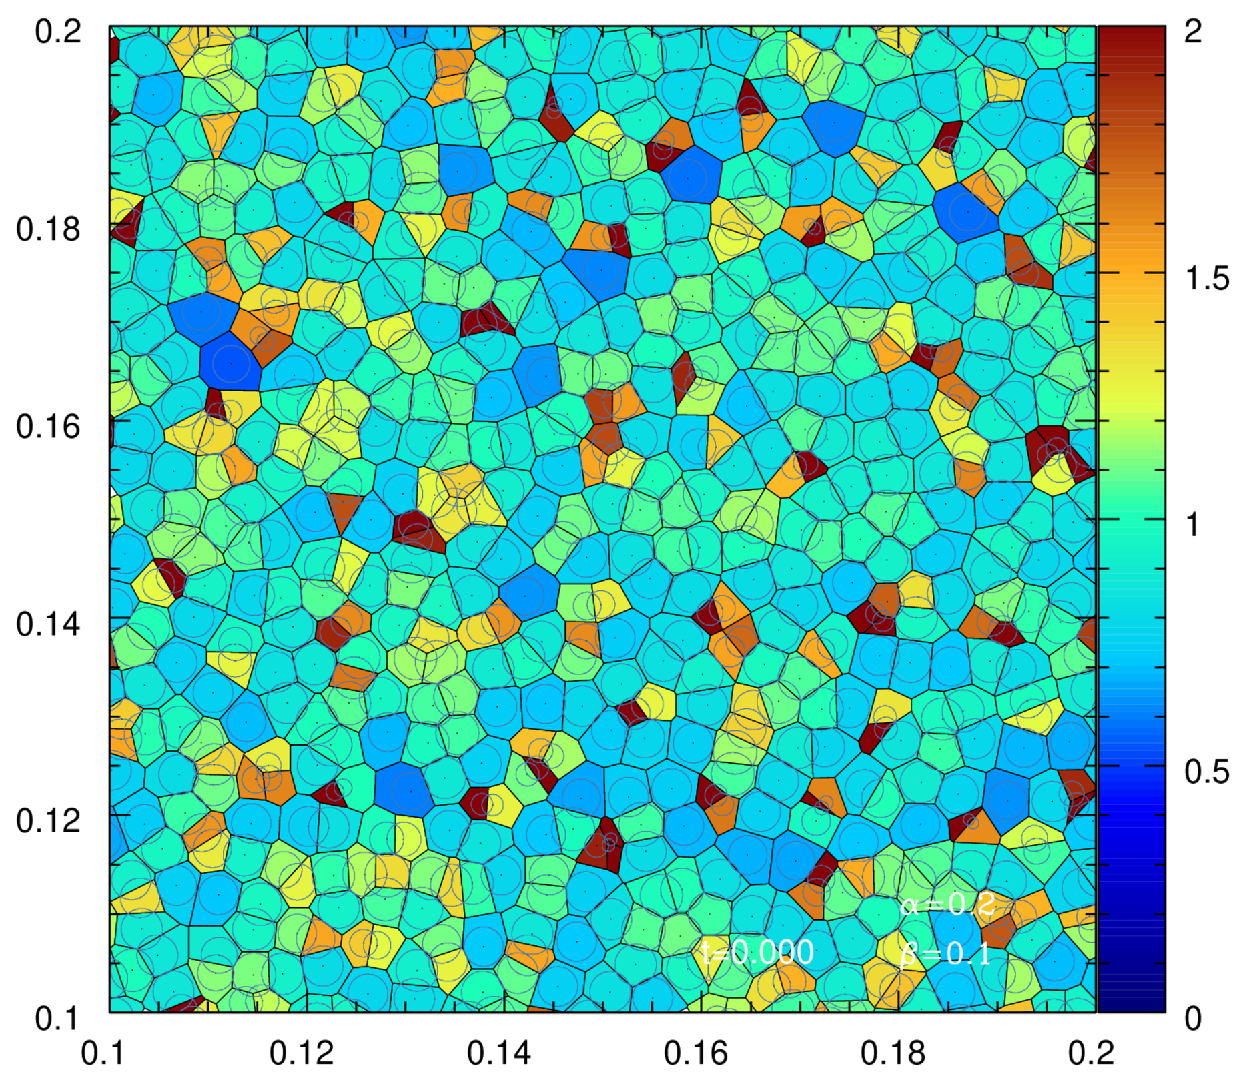
\includegraphics[width=\columnwidth]{2dvoro.pdf}	
\caption{Illustration of the two-dimensional Laguerre diagram. We semi-randomly distribute particles (shown in dots) of equal mass with their $w$ values shown with pale-blue circles. We adopt $\varkappa=0.55 $. Each diagram is color-coded to show the density. The density is normalized to the average.}
\label{voro2d}
\end{figure}


\section{Laguerre Face Velocity}
\subsection{Definitions and Setup}

Let two generator sites be defined by their positions $p$, $q$ and velocities $u_p$ and $u_q$. Each site has an associated weight $w_p, w_q$ with time derivatives $dw_p/dt$ and $dw_q/dt$.

We define the following geometric quantities:
\begin{itemize}
    \item {Unit normal vector} (pointing from $p$ to $q$): ${n} = \frac{q-p}{\|q-p\|}$
    \item {Intersection point} (where the radical plane intersects the line connecting $p$ and $q$):
    \begin{equation}
        m = {1\over2}\left({{p} + {q}} + \frac{w_p^2 - w_q^2}{\|q-p\|} n\right)
    \end{equation}
\end{itemize}

The {Radical Plane} is  the locus of points $x$ satisfying,
\begin{equation}
   \|{x} - {p}\|^2 - w_p^2 = \|{x} - {q}\|^2 - w_q^2
\end{equation}
from which we may derive the defining equation as,
\begin{equation}
    2{x} \cdot ({q} - {p}) = \|{q}|^2 - \|{p}\|^2 - w_q^2 + w_p^2.
\end{equation}

Differentiating both sides with respect to time $t$:
\begin{equation}
    {dx\over dt} \cdot ({q} - {p}) + {x} \cdot ({u}_q - {u}_p) = {q} \cdot {u}_q - {p} \cdot {u}_p - w_q{dw_q\over dt } + w_p {dw_p\over dt}
\end{equation}

Let ${dx\over dt} = {u}_\textrm{face}$. We are interested in the normal component $u_n = {u}_\textrm{face} \cdot {n}$. Dividing by $d$:
\begin{equation}
    u_n + {x} \cdot \frac{({u}_q - u_p)}{\|q-p\|} = \frac{{q} \cdot {u}_q - {p} \cdot {u}_p + (w_p{dw_p\over dt} - w_q{dw_q\over dt})}{\|q-p\|}
\end{equation}

Solving for $u_n$ and rearranging terms using dot products relative to the particle positions:
\begin{equation}
    u_n({x}) = {1\over \|q-p\|}\left[{{u}_p \cdot ({x} - {p}) - {u}_q \cdot ({x} - {q}) + \left(w_p{dw_p\over dt} - w_q{dw_q\over dt}\right)} \right]
\end{equation}

\subsection{Derivation of Tangential and Rotational Velocity}

Geometrically, the tangential velocity of an infinite plane is undefined. However, in the context of dynamic tessellations (like Voronoi/Laguerre moving meshes), the interface is assumed to move rigidly attached to the motion of the defining particles.

The total 3D velocity $u_\textrm{face}({x})$ is the sum of three components:
\begin{enumerate}
    \item {Normal Expansion:} The speed along the normal vector derived above.
    \item {Transverse Translation:} The average tangential velocity of the two particles.
    \item {Rotation (Tilting):} The rotation of the plane caused by the relative motion of particles perpendicular to the connecting axis.
\end{enumerate}

\subsection{Average Tangential Velocity (${\bar{u}}_{\perp}$)}
We extract the tangential components of the particle velocities:
\begin{align}
    {u}_{p,\perp} &= {u}_p - ({u}_p \cdot {n}){n} \\
    {u}_{q,\perp} &= {u}_q - ({u}_q \cdot {n}){n}
\end{align}
The plane translates tangentially with the average of these velocities:
\begin{equation}
    {\bar{u}}_{\perp} = \frac{{u}_{p,\perp} + {u}_{q,\perp}}{2}
\end{equation}

\subsection{Rotational Velocity (${u}_{rot}$)}
If ${u}_p \neq {u}_q$, the axis connecting the particles rotates. The angular velocity $\boldsymbol{\omega}$ of the axis ${d}_{pq}$ is given by the cross product of the normal and the relative velocity:
\begin{equation}
    \boldsymbol{\omega} = \frac{{n} \times ({u}_q - {u}_p)}{d}
\end{equation}

The plane rotates with this angular velocity around the anchor point ${m}$. The linear velocity due to rotation at a point $\vect{x}$ is:
\begin{equation}
    {u}_\textrm{rot}({x}) = \boldsymbol{\omega} \times ({x} - {m})
\end{equation}

\section{Final Formula: The 3D Velocity Vector}

Combining all components, the full 3-dimensional velocity vector ${u}_\textrm{face}({x})$ at any position ${x}$ on the radical plane is:

\begin{equation}
    u_\textrm{face}({x}) = 
    \underbrace{u_n({x}) {n}}_{\text{Normal}} + 
    \underbrace{\frac{{u}_{p,\perp} + {u}_{q,\perp}}{2}}_{\text{Tangential Translation}} + 
    \underbrace{\left[ \frac{{n} \times ({u}_q - {u}_p)}{d} \right] \times ({x} - {m})}_{\text{Rotation (Shear)}}
\end{equation}

Expanding the terms for computational implementation:

\begin{equation}
\boxed{
\begin{aligned}
    {u}_\textrm{face}({x}) = 
    & \left[ \frac{{u}_p \cdot ({x} - {p}) - {u}_q \cdot ({x} - {q}) + \frac{1}{2}\frac{d}{dt}(w_p^2 - w_q^2)}{d} \right] {n} \\
    & + \frac{1}{2} \left[ ({u}_p + {u}_q) - \left( ({u}_p + {u}_q) \cdot {n} \right) {n} \right] \\
    & + \frac{1}{d} \left[ {n} \times ({u}_q - {u}_p) \right] \times ({x} - {m})
\end{aligned}
}
\end{equation}


\section{The HLLC + Cullen--Dehnen Algorithm} \label{app:hllccd}

This appendix describes the complete HLLC + Cullen--Dehnen (CD10) algorithm
used as the baseline Laguerre scheme in the 1-D test suite.
The method combines an HLLC Riemann solver with a
time-dependent artificial-viscosity switch and MUSCL reconstruction,
integrated in time with a classical fourth-order Runge--Kutta (RK4) scheme.

\subsection{Cell Geometry and Conservation}

Each Lagrangian cell $p$ carries a fixed mass $m_p$.
In 1-D, the cell volume (length) is
$V_p = x_{p+\frac{1}{2}} - x_{p-\frac{1}{2}}$,
where $x_{p+\frac{1}{2}}$ is the face position between cells $p$ and $p\!+\!1$.
For Laguerre tessellation the face is shifted from the Voronoi midpoint by
the weight difference:
\begin{equation}
  x_{p+\frac{1}{2}}
  = \frac{x_p + x_{p+1}}{2}
  + \frac{\omega_p^2 - \omega_{p+1}^2}{2\,d_{p,p+1}},
\end{equation}
where $d_{p,p+1} = x_{p+1}-x_p$ and $\omega_p$ is the Laguerre weight
(power radius).
When $\omega=0$ for all cells, the tessellation reduces to the standard
Voronoi diagram.
The density is updated from $\rho_p = m_p / V_p$ and the
thermodynamic state follows from the ideal-gas equation of state,
$P_p = (\gamma-1)\rho_p e_p$ and
$c_p = \sqrt{\gamma P_p / \rho_p}$.


\subsection{MUSCL Reconstruction}

Before solving the Riemann problem at each face, we reconstruct the
left and right states using the MUSCL approach with the minmod limiter.
For a generic variable $\phi$ at cell $i$,
\begin{equation}
  \delta\phi_i = \mathrm{minmod}(\phi_i - \phi_{i-1},\;\phi_{i+1} - \phi_i),
\end{equation}
where
\begin{equation}
  \mathrm{minmod}(a,b) =
  \begin{cases}
    \mathrm{sgn}(a)\,\min(|a|,|b|), & ab > 0, \\
    0, & \text{otherwise}.
  \end{cases}
\end{equation}
The face states are then extrapolated as
\begin{equation}
  \phi_L = \phi_{i-1} + \tfrac{1}{2}\,\delta\phi_{i-1}, \qquad
  \phi_R = \phi_{i}   - \tfrac{1}{2}\,\delta\phi_{i}.
\end{equation}
This reconstruction is applied to the pressure $P$ and velocity $\vel$
at each internal face.


\subsection{HLLC Riemann Solver}

Given left/right states $(P_L, \vel_L, \rho_L, c_L)$ and
$(P_R, \vel_R, \rho_R, c_R)$, the HLLC solver
\citep[e.g.,][]{toro2009} first computes
a preliminary pressure estimate via the linearized (PVRS) solver,
\begin{equation}
  P_\text{pvrs}
  = \frac{Z_R P_L + Z_L P_R + Z_L Z_R (\vel_L - \vel_R)}{Z_L + Z_R},
\end{equation}
where $Z_{L,R} = \rho_{L,R}\,c_{L,R}$ are the acoustic impedances.
A shock correction factor is then applied to each side:
\begin{equation}
  q_K = \begin{cases}
    \sqrt{1 + \dfrac{\gamma+1}{2\gamma}\left(\dfrac{P_\text{pvrs}}{P_K}-1\right)}, & P_\text{pvrs} > P_K, \\[6pt]
    1, & \text{otherwise},
  \end{cases}
\end{equation}
for $K \in \{L,R\}$.
The weighted impedances $W_K = \rho_K c_K q_K$ yield the star-state
pressure and contact velocity:
\begin{equation}
  P^* = \frac{W_R P_L + W_L P_R + W_L W_R(\vel_L - \vel_R)}{W_L + W_R},
\end{equation}
\begin{equation}
  \vel^* = \frac{W_L \vel_L + W_R \vel_R + P_L - P_R}{W_L + W_R}.
\end{equation}
The face pressure is set to $P_{pq} = P^*$ and the face velocity to
$\vel_{pq} = \vel^*$.


\subsection{Cullen--Dehnen Viscosity Switch}

Following \citet{cullen2010}, a per-cell viscosity parameter
$\alpha_p$ is evolved in time.
The local activation is driven by the time derivative of the velocity
divergence:
\begin{equation}
  A_p = \max\!\left(0,\;
    -\frac{\nabla\!\cdot\!\vel_p^{(n)} - \nabla\!\cdot\!\vel_p^{(n-1)}}
          {\Delta t}\right),
\end{equation}
where the divergence is computed as
$\nabla\!\cdot\!\vel_p = (\vel_{p+\frac{1}{2}} - \vel_{p-\frac{1}{2}})/V_p$.
The target viscosity coefficient is
\begin{equation}\label{eq:alphaloc}
  \alpha_\mathrm{loc} = \alpha_\mathrm{max}\,
    \frac{h_p^2 A_p}{v_{s,p}^2 + h_p^2 A_p},
\end{equation}
where $h_p = V_p$ is the cell size and $v_{s,p}$ is the maximum signal
velocity seen by cell $p$ during the current RK4 step.
The evolution follows an asymmetric rule:
\begin{equation}\label{eq:alphacd}
  \alpha_p^{(n+1)} = \begin{cases}
    \alpha_\mathrm{loc}, & \alpha_\mathrm{loc} \ge \alpha_p^{(n)},\\[4pt]
    \alpha_\mathrm{loc} + (\alpha_p^{(n)} - \alpha_\mathrm{loc})\,
      e^{-\Delta t / \tau_p}, & \text{otherwise},
  \end{cases}
\end{equation}
with the decay timescale $\tau_p = h_p / (2\ell\,v_{s,p})$ and
$\ell$ a dimensionless parameter controlling the decay rate.
The coefficient is clamped to $[\alpha_\mathrm{min},\,\alpha_\mathrm{max}]$.

The face viscosity pressure is applied only in compression
($\Delta\vel = \vel_L - \vel_R > 0$):
\begin{equation}
  \Pi_{pq} = \tfrac{1}{2}\,\bar\alpha_{pq}\,v_{\mathrm{sig}}\,
    \bar\rho_{pq}\,\Delta\vel,
\end{equation}
where $\bar\alpha_{pq} = (\alpha_p + \alpha_q)/2$,
$\bar\rho_{pq} = (\rho_p+\rho_q)/2$, and the signal velocity is
\begin{equation}
  v_{\mathrm{sig}} = c_p + c_q + \beta\,\max(\Delta\vel,\,0).
\end{equation}
The total face pressure is $P_{pq} + \Pi_{pq}$.
In the present 1-D tests we use $\alpha_\mathrm{max}=1$,
$\ell=0.05$, $\alpha_\mathrm{min}=0$, and $\beta=1$.


\subsection{Flux Computation}

The semi-discrete equations of motion for each cell are:
\begin{align}
  \frac{d\vel_p}{dt} &= \frac{1}{m_p}
    \bigl(\mathcal{P}_{p-\frac{1}{2}} - \mathcal{P}_{p+\frac{1}{2}}\bigr),
    \label{eq:dvdt}\\[4pt]
  \frac{de_p}{dt} &= \frac{1}{m_p}
    \Bigl[\mathcal{P}_{p-\frac{1}{2}}
      \bigl(\vel_{p-\frac{1}{2}} - \vel_p\bigr)
    - \mathcal{P}_{p+\frac{1}{2}}
      \bigl(\vel_{p+\frac{1}{2}} - \vel_p\bigr)\Bigr],
    \label{eq:dedt}
\end{align}
where $\mathcal{P}_{p\pm\frac{1}{2}} = P^* + \Pi$ is the total face
pressure (HLLC star pressure plus artificial viscosity) and
$\vel_{p\pm\frac{1}{2}} = \vel^*$ is the HLLC contact velocity at
each face.
The position evolves as $dx_p/dt = \vel_p$.


\subsection{Boundary Conditions}

At a reflecting wall the face velocity is set to zero and
the wall pressure is computed from the
linearized Riemann condition:
\begin{equation}
  P_\mathrm{wall} = P_p \mp \rho_p c_p \vel_p,
\end{equation}
where the sign depends on the wall side
($-$ for the left wall, $+$ for the right).
For a transmissive boundary the face state is simply copied from
the adjacent cell: $P_\mathrm{face} = P_p$, $\vel_\mathrm{face} = \vel_p$.


\subsection{RK4 Time Integration}

The system is advanced with the standard four-stage Runge--Kutta method.
Let $\mathbf{U} = (x,\,\vel,\,e)$ denote the state vector.  Then:
\begin{align}
  \mathbf{k}_1 &= f(\mathbf{U}^n), \notag\\
  \mathbf{k}_2 &= f\!\left(\mathbf{U}^n + \tfrac{\Delta t}{2}\,\mathbf{k}_1\right), \notag\\
  \mathbf{k}_3 &= f\!\left(\mathbf{U}^n + \tfrac{\Delta t}{2}\,\mathbf{k}_2\right), \notag\\
  \mathbf{k}_4 &= f\!\left(\mathbf{U}^n + \Delta t\,\mathbf{k}_3\right),
\end{align}
\begin{equation}
  \mathbf{U}^{n+1} = \mathbf{U}^n
    + \frac{\Delta t}{6}\bigl(\mathbf{k}_1
      + 2\mathbf{k}_2 + 2\mathbf{k}_3 + \mathbf{k}_4\bigr).
\end{equation}
The cell geometry (face positions, volumes, densities) is recomputed
at every RK4 sub-stage.
The CD10 viscosity parameter $\alpha_p$ is updated once per full
timestep after the RK4 combination.

The global timestep is set by the CFL condition:
\begin{equation}
  \Delta t = C_\mathrm{cfl}\,\min_p
    \frac{V_p}{c_p + |\vel_p|},
\end{equation}
with $C_\mathrm{cfl} = 0.2$ for RK4.


\subsection{Algorithm Summary}

For each full timestep $\Delta t$:
\begin{enumerate}
  \item \textbf{RK4 sub-stages} ($s = 1,\ldots,4$):
    \begin{enumerate}[label=(\alph*)]
      \item Compute cell geometry:
            face positions $x_{p+\frac{1}{2}}$, volumes $V_p$,
            densities $\rho_p$, pressures $P_p$, sound speeds $c_p$.
      \item MUSCL reconstruction of $(P,\vel)$ at each face.
      \item HLLC Riemann solve $\rightarrow$ $(P^*,\vel^*)$ at each face.
      \item Evaluate CD10 viscosity $\Pi_{pq}$; accumulate $v_{s,p}$.
      \item Apply boundary conditions.
      \item Compute accelerations (eqs.~\ref{eq:dvdt}--\ref{eq:dedt})
            $\rightarrow$ stage derivative $\mathbf{k}_s$.
    \end{enumerate}
  \item \textbf{RK4 combination}: update $\mathbf{U}^{n+1}$.
  \item \textbf{CD10 $\alpha$ update}
        (eqs.~\ref{eq:alphaloc}--\ref{eq:alphacd}).
  \item \textbf{Timestep}: compute $\Delta t^{n+1}$ from CFL.
\end{enumerate}


\section{Shock Capturing with Adaptive Laguerre Weights} \label{app:shockcap}

In this appendix we document the stabilization methods
explored for the adaptive Laguerre weight ($\omega$) in the
presence of strong discontinuities.
All tests use the 1-D interacting blast-wave problem
(Woodward \& Colella 1984; $p_L=1000$, $p_M=0.01$,
$p_R=100$, $\gamma=1.4$, reflecting walls) with $N=200$
equal-mass particles and the HLLC Riemann solver with
the Cullen--Dehnen (2010) viscosity switch.

\subsection{Weight Function Modes}

Four weight prescriptions $\omega^2 = \varkappa_\omega \,d_{\rm mean}\,\psi(p)$
were tested, where the scaling function $\psi$ is:
\begin{enumerate}[label=(\roman*)]
  \item \textsc{Pressure}: $\psi = (P/P_0)^{(\gamma-1)/\gamma}$,
  \item \textsc{Enthalpy}: $\psi = (e + P/\rho)/h_0$,
  \item \textsc{SpecVol}: $\psi = (1/\rho)/v_0$,
  \item \textsc{CSound}: $\psi = c_s / c_0$.
\end{enumerate}
Here $P_0$, $h_0$, $v_0$, $c_0$ are reference scales set from the
initial conditions (geometric mean of IC pressures, etc.).
The \textsc{SpecVol} mode is the natural choice for equal-mass
Lagrangian particles because $V_i = m/\rho_i$, so
$\omega \propto 1/\rho$ makes the Laguerre cell volume track the
physical specific volume.

\subsection{Area-Adjustment (AA) Correction}

When the weight $\omega$ changes in time, the Laguerre face
shifts even without particle motion.  This changes the cell
volume and therefore the density, but the standard energy
equation does not account for the $P\,dV$ work of this
weight-induced compression or expansion.

The AA correction restores energy conservation by adding the
weight-change contribution to the face velocity:
\begin{equation}
  u_{f,\mathrm{AA}} = \frac{1}{2\,\Delta x}\left[
    \frac{d(w_p^2)}{dt} - \frac{d(w_q^2)}{dt}
    - \frac{(w_p^2-w_q^2)(u_q-u_p)}{\Delta x}\right],
\end{equation}
so that $u_f \to u_f + u_{f,\mathrm{AA}}$ in the Riemann problem
on each face.  The time derivatives are estimated by
finite difference:
\begin{equation}
  \frac{d(w_p^2)}{dt} \approx \frac{w_p^{2,n} - w_p^{2,n-1}}{\Delta t}.
\end{equation}
A limiter $|u_{f,\mathrm{AA}}| \le \alpha_{\rm AA}\, c_s$ is
applied to prevent overshoots, with $\alpha_{\rm AA}=1$ as the
default.

An analytical variant replaces the finite difference with
$d(\omega^2)/dt = -\beta\,\omega^2\,\nabla\cdot\vel$, where the
coefficient $\beta$ depends on the weight mode:
$\beta = \gamma-1$ (\textsc{CSound}),
$\beta = 2(\gamma-1)$ (\textsc{Pressure}, \textsc{Enthalpy}),
$\beta = -2$ (\textsc{SpecVol}).

\subsection{Tested Stabilization Methods}

\subsubsection{Method 1: Shock-Switch Weight Damping}
A compression-based switch detects shocks and reduces $\omega^2$
locally:
\begin{equation}
  \omega^2 \;\longleftarrow\; \frac{\omega^2}{1 + \kappa_s\, S^2},
  \qquad S \equiv \frac{\max(0,-\nabla\cdot\vel)\,d_{\rm mean}}{c_s},
\end{equation}
where $\kappa_s$ is the damping coefficient.  The dimensionless
shock indicator $S$ measures the compressive velocity divergence
in units of the sound crossing time.

\subsubsection{Method 2: Weight Relaxation}
Exponential smoothing of $\omega^2$ toward the target value
with a time constant $\tau = \tau_r\, d_{\rm mean}/c_s$:
\begin{equation}
  \omega^{2}_{\rm actual} = \omega^{2}_{\rm old}
    + \alpha_r\,(\omega^{2}_{\rm target} - \omega^{2}_{\rm old}),
  \qquad \alpha_r = \min\!\left(1,\;\frac{\Delta t}{\tau}\right).
\end{equation}
This prevents sudden jumps in $\omega^2$ and starts from
$\omega=0$ at $t=0$.

\subsubsection{Method 3: Weight Gradient Limiter}
An iterative smoother limits the spatial gradient of $\omega$:
\begin{equation}
  \left|\omega_i - \omega_j\right| \;\le\; g_{\max}\,\Delta x_{ij}
\end{equation}
for each neighboring pair $(i,j)$.  When violated, both weights are
pulled toward their mean by a factor $g_{\max}\Delta x / |\omega_i-\omega_j|$.
Three passes are applied per timestep.

\subsubsection{Method 4: Pressure-Ratio Threshold}
The shock-switch damping is activated only when the local
pressure ratio exceeds a threshold:
\begin{equation}
  \max\!\left(\frac{P_i}{P_j},\;\frac{P_j}{P_i}\right) > R_p^{\rm crit}
  \quad\text{for any neighbor } j.
\end{equation}
This is designed to leave moderate shocks (e.g.\ Shu--Osher)
unaffected while targeting extreme discontinuities
(e.g.\ interacting blast waves with $P$-ratio $\sim10^5$).

\subsection{Results on the Blast Problem}

\begin{table}[h!]
\caption{Blast-wave results for individual methods (\textit{without}
  AA correction).  All configurations use \textsc{CSound} weight mode
  with $\varkappa_\omega=0.1$--0.3 and face-shift limit 0.2--0.5.
  \textit{All entries failed} (hit 50\,000 step limit).}
\label{tab:blast_noaa}
\centering
\begin{tabular}{lcc}
\toprule
Method & Configs tested & Result \\
\midrule
Shock-switch alone    & 24 & All FAIL \\
Weight relaxation alone & 24 & All FAIL \\
Gradient limiter alone  & 24 & All FAIL \\
Combinations of above   & 36 & All FAIL \\
\bottomrule
\end{tabular}
\end{table}

\begin{table}[h!]
\caption{Blast-wave results with AA correction enabled.
  \textsc{SpecVol} weight mode, $\alpha_{\rm AA}=1.0$.}
\label{tab:blast_aa}
\centering
\begin{tabular}{lcccl}
\toprule
Configuration & $\varkappa_\omega$ & $\kappa_s$ & $L_1(\rho)$ & Status \\
\midrule
\textit{Base} ($\omega=0$)  & 0    & --- & 9.11e-2 & PASS \\
AA only              & 0.10 & 0   & ---      & FAIL \\
AA only              & 0.20 & 0   & ---      & FAIL \\
AA + $\kappa_s=5$    & 0.10 & 5   & 9.02e-2  & PASS $\star$ \\
AA + $\kappa_s=15$   & 0.08 & 15  & \textbf{8.58e-2}  & PASS $\star$ \\
AA + $\kappa_s=15$   & 0.10 & 15  & 9.76e-2  & PASS \\
AA + $\kappa_s=20$   & 0.10 & 20  & 9.62e-2  & PASS \\
AA + $\kappa_s=50$   & 0.08 & 50  & 8.66e-2  & PASS $\star$ \\
\bottomrule
\end{tabular}
\tablecomments{$\star$ denotes $L_1 < L_1^{\rm base}$.
The best result (boldface) improves upon the
unweighted baseline by 5.7\%.
The face-shift limit is $f_s=0.2$ for all entries.}
\end{table}

\subsection{Multi-Problem Assessment}

\begin{table*}[t!]
\caption{$L_1(\rho)$ across four test problems for selected
  configurations (HLLC+CD10, \textsc{SpecVol} weight, AA enabled).
  The \textit{base} row has $\omega=0$ (standard Lagrangian).}
\label{tab:multiproblem}
\centering
\begin{tabular}{lcccccc}
\toprule
Configuration & $\varkappa_\omega$ & $\kappa_s$ & Sod & Blast & Shu--Osher & Noh \\
\midrule
Base ($\omega\!=\!0$)    & 0    & ---  & 5.575e-3 & 9.11e-2  & 7.27e-1 & 6.14e-1 \\
AA only                  & 0.10 & 0    & 5.567e-3 & FAIL     & \textbf{6.35e-1} & 6.14e-1 \\
AA only                  & 0.20 & 0    & 5.569e-3 & FAIL     & \textbf{6.25e-1} & 6.14e-1 \\
AA + $\kappa_s\!=\!15$   & 0.08 & 15   & 5.571e-3 & \textbf{8.58e-2} & 7.79e-1 & 6.15e-1 \\
AA + $\kappa_s\!=\!0.5$  & 0.10 & 0.5  & 5.567e-3 & FAIL     & 6.40e-1 & 6.15e-1 \\
AA + $g_{\max}\!=\!0.5$  & 0.10 & 0    & 5.567e-3 & FAIL     & \textbf{6.32e-1} & 6.15e-1 \\
\bottomrule
\end{tabular}
\tablecomments{Bold entries indicate improvement over
the unweighted baseline.
AA-only configurations yield 12--14\% improvement on
Shu--Osher but fail on the blast problem.  Adding
shock-switch damping ($\kappa_s=15$) stabilizes the
blast but regresses Shu--Osher by $\sim$7\%.}
\end{table*}

\subsection{Discussion}

Two key findings emerge from these experiments:

\begin{enumerate}
  \item \textit{AA correction is necessary but not sufficient.}
    Without AA, the weight-induced volume change is not
    reflected in the energy equation, leading to a positive
    feedback loop at density discontinuities where $\omega$
    changes sharply.  With AA, energy is conserved
    and the Shu--Osher problem improves by 12--14\%.
    However, AA alone cannot stabilize the extreme pressure
    ratio ($\sim10^5$) of the blast problem.

  \item \textit{Shock-switch damping stabilizes extreme shocks
    at the cost of moderate-shock accuracy.}
    The blast instability originates at \textit{contact
    discontinuities} where the density gradient is large
    but $\nabla\cdot\vel \approx 0$.  The shock-switch
    ($S$-based) damping is only partially effective because
    it targets compressions rather than contacts.  A
    sufficiently strong damping coefficient ($\kappa_s \gtrsim 5$)
    is needed to stabilize the blast, but this
    indiscriminately suppresses the adaptive weight
    in moderate-shock regions (Shu--Osher), erasing the
    accuracy gain from the Laguerre tessellation.

\end{enumerate}

The fundamental trade-off is between adaptivity and stability:
the \textsc{SpecVol} weight naturally adjusts cell volumes
to track the physical specific volume ($V_i = m/\rho_i$),
providing excellent accuracy for smooth flows and moderate
shocks, but creating catastrophic face shifts at extreme
density jumps.  A contact-discontinuity--specific limiter
that preserves the weight in smooth regions while suppressing
it only at extreme density ratios remains an open problem.


\section{Sutherland--Hodgman Tessellation for GPU Acceleration}
\label{app:shtess}

In this appendix we describe an alternative polygon-clipping algorithm
for constructing 2D Laguerre cells and discuss why it is adopted for
the GPU implementation while the original incremental method is
retained on the CPU.

\subsection{Incremental Bisection (CPU)}

The in-house Laguerre tessellation implemented in \lageunha{} follows
the recursive bisection method described in Appendix~\ref{rbl}.  For
each generator~$i$ with weight $w_i$, the algorithm
\begin{enumerate}[nosep]
  \item sorts neighbouring generators by Laguerre distance
    $d_{\mathrm{rad}}^2 = \tfrac{1}{4}\,d^2(1+\Delta w/d^2)^2$,
  \item initialises a large bounding polygon (box),
  \item for each neighbour~$j$ in ascending $d_{\mathrm{rad}}^2$
    order, locates the two points where the Laguerre bisector of
    $(i,j)$ intersects the current polygon boundary (\emph{enter}
    and \emph{exit} points), then replaces the clipped portion with
    a single new face,
  \item terminates when the farthest surviving vertex is closer than
    the next neighbour's Laguerre distance.
\end{enumerate}
The polygon is stored as a \emph{doubly-linked circular list}
of \texttt{Voro2D\_Corner} nodes, each carrying vertex coordinates,
pointers to the upper/lower neighbour, and pointers to adjacent
corners.  The force loop traverses this linked list directly,
accessing face geometry and neighbour data through pointer chains:
\begin{equation}
  \texttt{tmp} \;\to\; \texttt{tmp->upperlink} \;\to\; \cdots
  \;\to\; \texttt{vorocorner}\,,
  \label{eq:lltraversal}
\end{equation}
so that tessellation and force evaluation share the same data
structure with no intermediate conversion.

This design is efficient on the CPU: each neighbour touches only the
two boundary vertices it clips, giving $O(N_{\rm neigh})$ work per
cell for an already-sorted neighbour list.  The linked-list storage
allows $O(1)$ insertion and deletion of corners.  OpenMP thread
safety is achieved by allocating one corner pool per thread
(or per cell-row).

\subsection{Sutherland--Hodgman Clipping (GPU)}

The incremental algorithm relies on three features that are
fundamentally incompatible with GPU execution:
\begin{itemize}[nosep]
  \item \emph{Pointer-based linked lists}: GPUs achieve throughput
    through coalesced memory access; pointer chasing across
    heap-allocated nodes destroys spatial locality.
  \item \emph{Dynamic memory allocation}: each
    \texttt{CreateNewCorner} call requires \texttt{malloc}; GPU
    \texttt{malloc} (device-side) is orders of magnitude slower
    than host \texttt{malloc} and serialises warps.
  \item \emph{Sequential polygon traversal}: finding the enter/exit
    points requires walking the linked list from an arbitrary active
    corner, creating warp divergence.
\end{itemize}

We therefore adopt the Sutherland--Hodgman (S-H) polygon clipping
algorithm \citep{1974CGIP....3..544S} for the GPU kernel.  S-H processes
each half-plane (bisector) by iterating over all edges of the current
polygon and classifying each edge--vertex pair as inside or outside:
\begin{enumerate}[nosep]
  \item \emph{Both inside}: output vertex~A unchanged.
  \item \emph{A inside, B outside}: output A, then the intersection.
  \item \emph{A outside, B inside}: output the intersection only.
  \item \emph{Both outside}: skip.
\end{enumerate}
The polygon is stored as a \emph{fixed-size array}
(\texttt{poly\_x[]}, \texttt{poly\_y[]}, \texttt{poly\_neigh[]}) in
GPU registers or local memory, requiring no dynamic allocation.
Neighbour data is gathered from a cell-linked-list CSR structure
and sorted by $d_{\mathrm{rad}}^2$ using an insertion sort (small $N$).

The Laguerre weight enters through the half-plane threshold.  For
neighbour~$j$ at relative position $(n_x, n_y)$ with
$d^2 = n_x^2 + n_y^2$, the weight fraction is
\begin{equation}
  f_w = \frac{1}{2} + \frac{w_i^2 - w_j^2}{2\,d^2}\,,
\end{equation}
and a polygon vertex $(v_x, v_y)$ lies inside the half-plane of
generator~$i$ if $v_x n_x + v_y n_y \le f_w \, d^2$.  When
$w_i = w_j$ this reduces to the standard Voronoi bisector at the
midpoint.

\subsubsection{Degenerate-Face Merging}

On a regular or near-regular grid, four (or more) Laguerre cells
meet at a single point.  The incremental algorithm handles this
naturally---the enter and exit points of a bisector coincide, so no
new face is created.  S-H, however, processes edges independently
and produces two nearly-identical vertices, creating a degenerate
face of near-zero area.  Because the CFL time step satisfies
$\Delta t \propto A_{\mathrm{face}} / v_{\mathrm{sig}}$, such
faces cause catastrophic time-step collapse.

We eliminate degenerate faces by a post-clipping vertex-merging pass.
After all bisectors have been applied, we scan adjacent vertices and
remove any pair separated by less than a relative threshold:
\begin{equation}
  |\Delta\vect{v}|^2 < \epsilon_{\mathrm{merge}}^2
  \equiv 10^{-6}\,\ell_{\max}^2\,,
  \label{eq:mergeeps}
\end{equation}
where $\ell_{\max}$ is the longest edge of the current polygon.  The
threshold $10^{-6}$ (i.e.\ edges shorter than $10^{-3}$
times the longest edge) was determined empirically by comparing GPU
and CPU face counts across $\sim\!10^5$ Laguerre cells on a
perturbed KH-instability grid (Section~\ref{app:shbench}).

\subsection{Thread Safety and Parallelism}

Both algorithms are embarrassingly parallel over generators: each
cell's tessellation depends only on the positions and weights of
neighbours within a bounded stencil.

\paragraph{CPU (OpenMP).}
The tessellation loop is parallelised over cell rows (\texttt{iy}).
Each thread owns a private corner pool (\texttt{Voro2D\_Corner
vorocorner[mp]}) and allocates per-cell neighbour work arrays.
Race conditions are avoided because the output (volume, density,
gradients, stress) is written to each particle's own struct fields.

\paragraph{GPU (CUDA).}
One CUDA thread processes one generator.  The kernel
\texttt{voronoi\_tessellate\_kernel} gathers neighbours from a
$3\times3$ cell stencil stored in CSR format, performs S-H clipping,
vertex merging, and computes volume, density, pressure, sound speed,
and (when $\texttt{av\_mode}\ge 1$) velocity gradients and NS stress---all
within a single kernel launch.  The resulting polygon is written to a
\texttt{PolygonOut} buffer (fixed $48$~corners per particle), then a
second kernel (\texttt{scatter\_faces\_kernel}) converts the polygon
vertices into a global \texttt{FaceCSR} structure (CSR-formatted face
connectivity and geometry) consumed directly by the GPU force kernel.

\subsection{Performance Comparison}
\label{app:shbench}

Table~\ref{tab:tessbench} summarises the tessellation cost for
$N_x=256$ ($131{,}072$ particles) on a single MPI rank.
The S-H algorithm is approximately 13\% faster than the incremental
method on the CPU, owing to cache-friendly array traversal versus
pointer-chasing through the linked list.  Memory usage per thread is
comparable: ${\sim}7$~KB (S-H, stack arrays) versus ${\sim}70$~KB
(incremental, corner pool), but in both cases the dominant allocation
is the shared neighbour array (${\sim}5$~KB per cell).
The GPU kernel achieves an additional $3$--$4\times$ speedup over
the CPU S-H, and when combined with the GPU force kernel the
full-step acceleration reaches $24\times$ for \texttt{av\_mode\,=\,0}.

\begin{table}[h]
\caption{Tessellation time for the KH test ($N_x=256$, single rank,
single thread for CPU).  ``Incremental'' is the in-house recursive
bisection; ``S-H'' is Sutherland--Hodgman on the same CPU.
\label{tab:tessbench}}
\begin{tabular}{lrrr}
\toprule
Method & Time (ms) & Faces & Speedup \\
\midrule
Incremental (CPU) & 1085 & 524\,288 & 1.0$\times$ \\
S-H (CPU)         &  956 & 524\,288 & 1.1$\times$ \\
S-H (GPU, RTX 5000 Ada) & 270 & 524\,288 & 4.0$\times$ \\
\bottomrule
\end{tabular}
\end{table}

The S-H method produces identical face counts and total cell volumes
to the incremental method on the initial (regular) grid.  After
particles have moved, the GPU S-H generates $\sim\!7$\% more faces
than the CPU incremental method; the extra faces are near-degenerate
edges at grid corners that survive the merging threshold
\eqref{eq:mergeeps}.  These contribute negligibly to the volume
integral and do not affect the CFL time step once the merging
threshold is applied.

\subsection{Design Rationale}

Given the modest 13\% CPU speedup and the significant refactoring
cost---the force loop (\texttt{getAccVoro2DBlend}) is tightly
coupled to the linked-list corner traversal \eqref{eq:lltraversal},
requiring a full rewrite to accept array-based face data---we retain
the incremental method for all CPU code paths.  The S-H algorithm is
used exclusively on the GPU, where the array-based \texttt{FaceCSR}
format is the natural interface to the force kernel.  This hybrid
design allows both paths to coexist: the CPU path serves as a
reference implementation and fallback, while the GPU path provides
the production-level throughput needed for large simulations.


\bibliographystyle{aasjournal}

\bibliography{reference}







\end{document}





